% =========================================================================
% DefectSegAM — full-length manuscript for Additive Manufacturing (Elsevier)
% Korean working copy (internal review). The English submission version will
% be produced from this file once the content is final; keep sentence
% structure translation-friendly. Journal-mandated headings (end matter)
% are kept in English; prose is Korean.
% Build: pdflatex main && bibtex main && pdflatex main && pdflatex main
% Section files live in sections/ and are \input fragments (no preamble).
% =========================================================================
\documentclass[preprint,12pt]{elsarticle}

\usepackage{graphicx}
\usepackage{kotex}
\usepackage{booktabs}
\usepackage{tabularx}
\usepackage{makecell}   % two-line column headings (\makecell) in tables
\usepackage{amsmath}
\usepackage{amssymb}
\usepackage{multirow}
\usepackage{xcolor}
\usepackage{hyperref}

% Numbered references in order of first citation (elsarticle default;
% elsarticle-num handles the list format). Compressed citation ranges
% ([1-3]) can be enabled at submission time with the natbib option
% "sort" + "compress" via \biboptions{}; it is left off here because the
% static checker flags the option string's ampersand as a stray '&'.

% ---- Manuscript-wide macros --------------------------------------------
% Red bracketed TODO marker for planned-but-not-yet-run experiments and
% metadata that must be verified before submission.
\newcommand{\TODO}[1]{\textcolor{red}{[TODO: #1]}}
\DeclareMathOperator*{\argmax}{arg\,max}

% ---- Page-layout tuning (Korean working copy) ----------------------------
% kotex's inter-syllable glue has no stretch, so pdfTeX gives up on some
% mostly-Hangul lines (Overfull \hbox) unless an emergency pass is allowed.
\setlength{\emergencystretch}{2em}
% LaTeX's default \topfraction=0.7 strands any [t] float taller than
% 0.7*\textheight (384 pt here) -- and every later float of the same kind --
% until the end of the document. Allow tall tables at page tops; floats that
% fill a page on their own use [tp] instead.
\renewcommand{\topfraction}{0.9}
\renewcommand{\textfraction}{0.1}

\journal{Additive Manufacturing}

\begin{document}

\begin{frontmatter}

% Original English title:
% DefectSegAM: Label-efficient layer-wise defect segmentation for
% powder bed fusion additive manufacturing with a frozen vision foundation
% model and cross-machine generalization
\title{DefectSegAM: 고정(frozen) 비전 파운데이션 모델을 활용한 분말 베드 융합
적층제조의 라벨 효율적 레이어 단위 결함 분할 및 교차 장비
일반화\tnoteref{abbr}}

% Elsevier: abbreviations that are not standard in the field are listed in a
% footnote on the first page and defined again at first use in the text.
\tnotetext[abbr]{약어: AM, additive manufacturing(적층제조); PBF, powder bed
fusion(분말 베드 융합); L-PBF, laser powder bed fusion(ISO/ASTM 52900 표기
PBF-LB/M); BJ, binder jetting; DSCNN, dynamic segmentation convolutional
neural network; DPT, dense prediction transformer; ViT, vision transformer;
VPPM, voxel-wise property prediction model; GT, ground truth; IoU/mIoU,
(mean) intersection-over-union; TTA, test-time augmentation; EMA,
exponential moving average; DDP, distributed data parallelism; XCT, X-ray
computed tomography; RMSE, root-mean-square error; YS/UTS/UE/TE, yield
strength / ultimate tensile strength / uniform elongation / total
elongation.}

\author[aff1]{Taehoon Lee\corref{cor1}}
\ead{lth9029@gmail.com}
\cortext[cor1]{교신저자.}
% TODO: co-author list to be finalized. Kept as a comment (not \TODO) because
% elsarticle propagates the \author field into running heads and PDF metadata.
% TODO: replace the gmail address with an institutional e-mail before
% submission (journal requirement; see handoff).

\affiliation[aff1]{organization={\TODO{소속
(학과, 기관)}},
            city={\TODO{도시}},
            country={\TODO{국가}}}

\begin{abstract}
레이어 단위 분말 베드 영상은 분말 베드 융합(powder bed fusion, PBF)
적층제조에서 가장 널리 사용되는 in-situ 모니터링 방식 중 하나이지만,
픽셀 단위 결함 분할(defect segmentation)은 전문가가 주석한 이미지의
부족과 장비, 재료, 카메라 구성 간의 낮은 전이 성능으로 인해 여전히
제한적이다. 본 연구에서는 고정된(frozen) DINOv2 비전 트랜스포머
인코더(86\,M 파라미터)에 학습 파라미터가 14.6\,M에 불과한 경량
dense prediction transformer (DPT) 방식 디코더를 결합하고, 각 레이어의
용융 직후 이미지와 분말 도포 직후 이미지를 명시적 변화 단서---두 시점
간의 특징 차이---를 통해 융합하여 11-class 결함 맵을 생성하는
세그멘테이션 네트워크인 DefectSegAM을 제안한다. 2단계의 라벨
효율적(label-efficient) 학습 절차는 먼저 운영 세그멘테이션 모델이 의사
라벨(pseudo-label)을 부여한 12{,}607개 빌드 레이어에서 디코더를
사전학습한 뒤, 레이저 PBF와 바인더 젯팅(binder jetting)을 아우르는 8개
장비/재료 소스에서 추출한 단 125개의 전문가 주석 레이어만으로
미세조정한다. 아울러 실험과는 별도로, 기존 결함 어휘에 혼재된 원인
기준과 외형 기준을 분리하여 레이어 이미지에 나타난 특징을 판정 기준으로
정의한 분류 체계를 향후 어노테이션을 위해 제안한다. 평가를
위해서는 dynamic segmentation convolutional
neural network (DSCNN) 베이스라인의 충실한 재구현과 비교하는 held-out
사람
정답(human ground truth) 프로토콜을 규정하였으며, 이 프로토콜은 레이저
PBF와 binder jetting을 아우르고 저자들이 현재 수집·픽셀 라벨링 중인
Veltz M160/M280 및 EOS 장비의 교차 장비(cross-machine) 세트를
포함한다 \TODO{held-out 세그멘테이션 결과 산출 예정}. 다운스트림
검증으로서, 그 외 조건이 동일한 인장 특성 예측 파이프라인에서
데이터셋이 제공하는 DSCNN 맵을 DefectSegAM 출력으로 교체하면
6{,}373개 시편에 대한 인장강도(ultimate tensile strength)의 평균 제곱근
오차(root-mean-square error, RMSE)가 70.7\,MPa---단순 전역 평균 예측기의
68.4\,MPa보다도 나쁜 수준---에서 37.5\,MPa로 감소하며, 이는 단순
베이스라인 대비 45.2\,\% 감소에 해당함을 확인하였다.
\end{abstract}

% Research highlights (Elsevier: 3-5 bullets, each <= 85 characters including
% spaces in the English version; no jargon or abbreviations; submitted as a
% separate file at submission, rendered here by elsarticle as a preliminary
% page). English wording for the submission version and its length:
%  1. A frozen vision foundation encoder and a light decoder segment powder
%     bed layers                                                        (80)
%  2. Explicit melt-to-spread change cues fuse the two camera views of every
%     layer                                                             (76)
%  3. Pseudo-label pretraining plus fine-tuning on only 125 expert-labelled
%     layers                                                            (76)
%  4. Human ground truth never used in training spans laser and binder jet
%     machines                                                          (77)
%  5. Swapping the incumbent defect maps cuts tensile strength error from
%     70.7 to 37.5 MPa                                                  (84)
\begin{highlights}
\item 고정된 비전 파운데이션 인코더와 경량 디코더로 분말 베드 레이어의
      결함을 분할한다
\item 용융--도포 간 명시적 변화 단서로 각 레이어의 두 카메라 시점을
      융합한다
\item 의사 라벨 사전학습에 단 125개 전문가 주석 레이어의 미세조정을
      결합한다
\item 학습에 쓰지 않은 사람 정답으로 레이저 및 바인더 젯 장비 전반을
      평가한다
\item 기존 결함 맵을 교체하면 인장강도 예측 오차가 70.7에서 37.5\,MPa로
      낮아진다
\end{highlights}

% Keywords: at most 6 (Elsevier guidance ranges 1-7; 6 is the safe
% intersection); ISO/ASTM 52900 process names.
\begin{keyword}
적층제조(Additive manufacturing) \sep 레이저 분말 베드
융합(Laser powder bed fusion) \sep In-situ 모니터링(In-situ monitoring)
\sep 결함 분할(Defect segmentation) \sep 비전 파운데이션
모델(Vision foundation model) \sep 딥러닝(Deep learning)
\end{keyword}

\end{frontmatter}

% =========================================================================
% Section 1 — Introduction (Korean translation)
% File: sections/1_introduction.tex  (\input fragment; no \documentclass)
% Model name: DefectSegAM (exact spelling, everywhere)
% =========================================================================

\section{서론}
\label{sec:intro}

금속 적층제조(additive manufacturing, AM)는 시제품 제작 단계를 넘어 본격적인
양산 단계로 확고히 이동하고 있다. 글로벌 AM 시장은 2023년 200.35억~USD 규모에
도달하여 전년 대비 11.1\% 성장하였고, 금속 AM 장비는 2022년 3{,}049대에서
2023년 3{,}793대로 판매량이 증가하였다~\cite{Wohlers2024}. 이를 보완하는 산업
분석에서는 산업용 AM 시장을 2023년 105.0억~EUR 규모로 평가하고 2028년까지
연평균 13.9\%의 성장률을 전망하였으며, 금속 AM이 폴리머 AM보다 약 두 배
빠르게 성장할 것으로 예측하였다~\cite{AMPOWER2024}. 레이저 분말 베드
융합(laser powder bed fusion, L-PBF; ISO/ASTM 52900 표기로는
PBF-LB/M)~\cite{ISO52900,Gibson2021AMTech,King2015LPBF}은
항공우주 및 생체의료 분야에서 높은 가치를 갖는 기하학적 자유도와 함께
근사 최종 형상(near-net-shape)의 금속 부품을 제작할 수 있기 때문에 이러한
성장의 상당 부분을 차지한다~\cite{BlakeyMilner2021Aerospace,Bose2018Biomaterials}.
그러나 동일한 층별 용융 공정은 키홀 기공(keyhole
porosity)~\cite{King2014Keyhole}, 용융 부족(lack of
fusion)~\cite{Tang2017LOF}, 스패터(spatter) 비산~\cite{Ly2017Spatter}, 그리고
리코터--파트 간섭과 같은 확률적 결함 형성에 취약하며, 이러한 결함의 발생은
국소 형상과 공정 이력에 민감하게 결합되어
있다~\cite{Sames2016Metallurgy,DebRoy2018PMS}. 그 결과 명목상 동일한 부품이라도
기계적 성능이 서로 다를 수 있으므로, 오늘날의 인증은 witness 시편의 파괴
시험과 X-ray computed tomography
(XCT)~\cite{Seifi2016Qualification,Seifi2017Standardization,duPlessis2018XCT}에
크게 의존하며, 이러한 부품 단위 검사 부담은 산업적 확산을 가로막는 주요 비용
장벽으로 널리 지목되고 있다.

레이어 단위 in-situ 이미징은 이러한 부담에 대응할 수 있는 가장 폭넓게 이용
가능한 수단이다. 산업용 L-PBF 장비는 레이어마다 두 번---레이저 노광 직후 한
번과 분말 도포 직후 한 번---분말 베드를 촬영할 수 있으므로, 모든 빌드는
사실상 추가 비용 없이 자기 자신의 제조 과정에 대한 공간적으로 정합된 시각
기록을 남긴다~\cite{Scime2018Anomaly,Gobert2018InProcess,DebRoy2021NatRevMater,Mahmoud2021LPBFreview}.
이 기록을 활용하는 여러 방법 가운데 분말 베드 이상 영역의 픽셀 단위 의미
분할(semantic segmentation)은 두 가지 이유에서 특히 가치가 있다. 첫째, 공정
제어 측면에서, 픽셀 단위 결함 맵은 도포 및 용융 이상을 빌드 평면과 적층
방향을 따라 국소화하여 레이어 수준의 개입을 지원하며, 그 클래스별 구조는
리코터 줄무늬(streaking)와 같은 장비 상태 신호를 과용융·불완전 용융과 같은
에너지 밀도 신호로부터 분리해 낸다~\cite{Scime2020DSCNN}. 둘째, 물성 예측
측면에서, Scime 등은 세그멘테이션 맵의 슈퍼복셀(supervoxel) 집계량을 다른
in-situ 피처와 결합하면 6{,}299개 시편에 걸쳐 국소 인장 특성을 예측할 수
있음을 보였다~\cite{VPPM_Baseline,ORNL_CoRegistered_Dataset}. 그러나
세그멘테이션 정보원은 하류의 모든 것을 제한한다.
Section~\ref{sec:results}에서 보이듯이, 그 외 모든 조건이 동일한 물성 예측
파이프라인에 배포된 dynamic segmentation convolutional neural network
(DSCNN)~\cite{Scime2020DSCNN}가 데이터셋에 제공한 결함 채널만을 입력하면
인장강도(ultimate tensile strength, UTS) 예측의 평균 제곱근
오차(root-mean-square error, RMSE)가 단순(naive) 전역 평균 예측기보다도 나쁜
수준으로 붕괴하는 반면, 동일한 파이프라인에 본 논문이 제안하는 모델의 결함
맵을 입력하면 그 오차가 단순 예측기 대비 절반 가까이 줄어든다.

더 나은 분말 베드 세그멘테이션을 가로막는 중심 장애물은 어노테이션 부족이다.
수 메가픽셀 규모의 레이어 이미지를 전문가가 픽셀 단위로 라벨링하는 작업은
느리고, 그 결과로 공개된 코퍼스의 규모는 작다: Peregrine v2021-03 릴리스는
20개의 전문가 어노테이션 L-PBF 레이어를 포함하며~\cite{Peregrine_v2021_03},
v2022-10 릴리스의 여섯 개 장비--소재 조합은 각각 5개에서 26개의 어노테이션
레이어를 제공한다~\cite{Peregrine_v2022_10}. 본 연구에서 사용한 여덟 개
소스를 모두 합해도 사람이 어노테이션한 레이어는 125개에 불과하다. 한편
이미지의 외관은 장비, 광학계, 조명, 소재에 따라 크게 달라지므로, 한 플랫폼의
수십 개 레이어만으로 처음부터 학습된 세그멘테이션 네트워크는 심각한 과적합
위험과 함께, 다른 플랫폼으로 전이될 때 고전적인 데이터셋 시프트(dataset
shift) 페널티를 동시에 떠안는다~\cite{Quinonero2009DatasetShift,Torralba2011DatasetBias,Pan2010TransferLearning}.
이에 대한 사실상의 표준적 대응---DSCNN--Peregrine
계열~\cite{Scime2020DSCNN}과 같이 장비마다 별도의 지도학습 모델을 학습하는
방식---은 라벨링 비용을 장비 대수만큼 배가시킨다.

본 논문은 고정된(frozen) 자기지도 비전 파운데이션 모델(foundation model) 위에
구축된 분말 베드 결함 세그멘테이션 모델인 \textbf{DefectSegAM}을
제안한다(Fig.~\ref{fig:architecture}). 레지스터 토큰(register token)을 갖는
DINOv2 ViT-B/14 인코더~\cite{Oquab2024DINOv2,Darcet2024Registers}는 전체가
고정된 채 유지되며, 네 개의 트랜스포머 깊이에서 추출된 피처는 레이어당 두
장의 이미지(용융 직후와 도포 직후)에 걸쳐 융합되고---이때 베드의 용융 유발
변화를 인코딩하는 명시적인 이미지 간 차분(difference) 항을 포함한다---DPT
방식의 다중 스케일 디코더~\cite{Ranftl2021DPT}로 디코딩된다. 고정된 86~M개의
백본 파라미터 위에서 디코더와 헤드의 14.6~M개 파라미터만이 학습된다. 학습은
라벨 효율적인 두 단계로 진행된다: Stage~1에서는 ORNL co-registered
데이터셋~\cite{ORNL_CoRegistered_Dataset}의 다섯 개 빌드 중 네 개에서 추출한
12{,}607개의 미어노테이션 양산 레이어에 대해, 배포된 DSCNN의 자체 예측을
비용이 들지 않는 의사 라벨(pseudo-label)로 사용하는 지식 증류(knowledge
distillation)로 디코더를 사전학습하고, Stage~2에서는 여섯 개의 L-PBF 소스와
두 개의 바인더 젯팅(binder jetting) 소스에서 취합되어 통일된 11-클래스
온톨로지(Table~\ref{tab:classes})로 재매핑된 사람 어노테이션 레이어에 대해
미세조정한다~\cite{Peregrine_v2021_03,Peregrine_v2022_10}. ORNL 코퍼스의
극단적인 클래스 불균형(Section~\ref{sec:method-problem})은
역빈도(inverse-frequency) 클래스 인지 샘플링, Copy-Paste
증강~\cite{Ghiasi2021CopyPaste}, focal
loss~\cite{Lin2017FocalLoss}로 대응한다. 아울러 향후 어노테이션을 위한
외형 기준(appearance-based) 결함 분류 체계를
제안한다(Section~\ref{sec:method-taxonomy}).

평가 설계에서는, ORNL 양산 빌드의 밀집 라벨이 DSCNN의 예측이어서 해당 빌드의
지표가 교사(teacher) 일치도에 그치므로(Section~\ref{sec:setup-metrics}), 정확도
주장은 모든 학습에서 제외된(held-out) 사람 ground truth만을 기준으로 한다:
(i) 외부 2025 Peregrine held-out
세트~\cite{Peregrine_v2025_TODO}(Section~\ref{sec:setup-heldout-peregrine}),
그리고 (ii) 장비 간(cross-machine) 일반화를 검증하기 위해 저자들이 현재
수집 및 픽셀 라벨링을 진행하고 있는 Veltz M160 및 M280 장비와 EOS PBF
장비의 리코팅 이미지(Section~\ref{sec:setup-heldout-crossmachine})가
그것이다. DefectSegAM과 동일한 데이터로 학습한
DSCNN~\cite{Scime2020DSCNN}의 충실한 재구현을 주요 베이스라인으로 사용한다. \TODO{held-out 사람 GT 실험과 장비 간
실험(Sections~\ref{sec:results-heldout}
및~\ref{sec:results-crossmachine})은 계획되어
있으나 아직 수행되지 않았다; 결과가 나오는 대로 이 문단에 대표 수치를 삽입할
것.}

본 연구의 기여는 다음과 같다.
\begin{enumerate}
  \item \textbf{아키텍처.} 각 레이어의 도포 직후 이미지와 용융 직후 이미지에
        공유되는, 레지스터 토큰을 갖는 고정 DINOv2 ViT-B/14 인코더를,
        명시적 차분 항을 포함하는 단계별(per-stage) 이중 이미지 융합 및 DPT
        방식 다중 스케일 디코더와 결합한 DefectSegAM을 제안한다. 고정 백본
        위에서 디코더와 헤드만이 학습되므로, 시각 표현은 플랫폼마다 다시
        학습되는 대신 장비와 소재 전반에 걸쳐 상각(amortize)된다.
  \item \textbf{라벨 효율적 2단계 학습.} 배포된 양산 모델의 의사 라벨
        레이어로부터의 지식 증류와, 통일된 11-클래스 온톨로지 아래 여덟 개의
        이종 장비--소재 소스에서 취합한 소규모 사람 어노테이션 레이어에 대한
        미세조정을 결합하고, 여러 자릿수에 걸쳐
        차이 나는 클래스별 픽셀 수에는 클래스 인지 샘플링, Copy-Paste 증강,
        focal loss로 대응한다.
  \item \textbf{Held-out 사람 GT 평가 프로토콜.} 사람 GT만을 정확도의
        기준으로 삼는 평가 스위트를 명시한다: 학습에 전혀 사용되지 않은
        외부 2025 Peregrine 사람 어노테이션 벤치마크, Veltz M160/M280 및
        EOS PBF 장비의 장비 간 테스트 이미지(수집 및 라벨링 진행 중),
        그리고 동일한 데이터로 충실히 재구현·학습된 DSCNN 베이스라인이
        그것이다.
        \TODO{프로토콜은 정의되었으나 실험은
        미수행(Section~\ref{sec:setup}).}
  \item \textbf{하류 유용성 사례 연구.} 이미 발표된 인장 특성 예측
        파이프라인 전체를 고정한 채 세그멘테이션 정보원만을 교체하는 실험을
        통해, 데이터셋이 제공하는 DSCNN 맵은 단순 전역 평균 예측기 아래로
        붕괴하는 반면(UTS RMSE 70.7 대 68.4~MPa), DefectSegAM 맵은 단순
        베이스라인 대비 45.2\% 낮은 37.5~MPa에 도달하며 네 가지 인장 특성
        모두에서 개선을 보임을 확인한다(Section~\ref{sec:results-downstream}).
  \item \textbf{외형 기준 결함 분류 체계(부수적 제안).} 실험과 별도로,
        Peregrine 어휘에 혼재된 원인 기준과 외형 기준을 분리하여 레이어
        이미지 특징을 판정 기준으로 정의한 결함 8종(Under Melting 처리 확정 전
        기준)과 배경 2종의 체계를 향후 어노테이션을 위해 제안하고, 기존
        라벨 공간 및 ASTM E3353-22 용어와의
        대응(Table~\ref{tab:taxonomy})과 데이터 가용성을
        정리한다(Section~\ref{sec:method-taxonomy}).
        \TODO{제안 체계로 재어노테이션한 뒤 재학습·재평가할
        것(Section~\ref{sec:method-taxonomy}).}
\end{enumerate}

본 논문의 나머지 부분은 다음과 같이 구성된다. Section~\ref{sec:related}에서는
분말 베드 모니터링, ex-situ 라벨 기반 결함 검출, AM 분야의 파운데이션 모델,
결함-물성 모델링에 관한 관련 연구를 검토하고 연구 공백을 종합한다.
Section~\ref{sec:method}에서는 문제 설정과 실험용 11-클래스 온톨로지,
제안하는 외형 기준 결함 분류 체계, DefectSegAM의 아키텍처, 2단계 학습
레시피, 클래스 불균형 대응 전략, 그리고 증강·추론·후처리 파이프라인을
차례로 상술한다. Section~\ref{sec:setup}에서는 데이터셋, held-out 사람 GT
평가 프로토콜, 베이스라인, 평가 지표, 구현 세부사항과 다운스트림 물성
예측 설정을 기술한다. Section~\ref{sec:results}에서는 세그멘테이션 및 하류
물성 예측 결과를 보고하고, Section~\ref{sec:discussion}에서는 한계와 시사점을
논의하며, Section~\ref{sec:conclusion}에서 결론을 맺는다.

% =========================================================================
% Section 2 — Related Work (Korean translation)
% File: sections/2_related_work.tex  (\input fragment; no \documentclass)
% Model name: DefectSegAM (exact spelling, everywhere)
% =========================================================================

\section{관련 연구}
\label{sec:related}

\subsection{레이어 단위 분말 베드 모니터링과 DSCNN--Peregrine 계열}
\label{sec:related-monitoring}

초기의 in-situ 모니터링은 결함 검출을 공정 수준의 신호 분류 문제로 다루었다.
Okaro 등은 49개 인장 바(tensile bar)에서 획득한 광다이오드 신호로
준지도(semi-supervised) 모델을 학습하여 약 77\%의 성공률로 불량 공정을
판별하였고~\cite{Okaro2019SemiSup}, Baumgartl 등은 H13 공구강의 off-axis
적외선 서모그램을 경량 합성곱 네트워크로 분류하여 평균 균형 정확도(mean
balanced accuracy) 96.8\%를 달성하였다~\cite{Baumgartl2020IRCNN}. 이러한
분류기는 적시에 경보를 제공하지만 결함을 국소화하지는 못한다. 공간 분해능은
레이어 단위 분말 베드 촬영 및 용융풀(melt-pool) 이미징과 함께 확보되기
시작하였다: Scime와 Beuth는 엔지니어링된 컴퓨터 비전 피처로 여섯 가지 분말
베드 이상 유형을 분류하였고~\cite{Scime2018Anomaly}, Inconel~718에 대해
용융풀 형태를 키홀 및 balling 영역과 연관지었으며~\cite{Scime2019MeltPool},
Gobert 등은 다중 모달 통합 후 약 85\%의 정확도로 서포트 벡터 머신을 이용해
고해상도 레이어 이미지의 불연속(discontinuity)을
검출하였다~\cite{Gobert2018InProcess}.

Scime 등의 DSCNN~\cite{Scime2020DSCNN}은 이 연구 계열을 여덟 개 클래스
온톨로지를 갖는 단일한 장비 불특정(machine-agnostic) 픽셀 단위 분말 베드
세그멘테이션 모델로 통합하였다 \TODO{투고 전에 원저 DSCNN의 학습 데이터
규모(픽셀, 레이어, 빌드 수)를 2020년 논문과 대조하여 검증할 것}.
Peregrine 모니터링 플랫폼에 배포되어 ORNL Co-Registered 데이터셋(Peregrine
v2023-11)~\cite{ORNL_CoRegistered_Dataset}과 함께 제공되는 양산 후속 모델은
온톨로지를 12개 클래스로 확장하고(recoater hopping, incomplete spreading,
misprint, under-melting 추가) 모든 레이어에 대해 $1842\times1842$ 크기의
클래스별 마스크를 생성한다. 이 온톨로지의 클래스는 관찰되는 이미지에
따라 개략적으로 갓 도포된 분말 베드의 이상(recoater hopping, recoater
streaking, incomplete spreading, debris), 용융된 표면의 이상(spatter,
misprint, 키홀 전조로서의 over-melting, lack-of-fusion 전조로서의
under-melting), 그리고 두 이미지 모두에서 관찰되는 이상(swelling,
super-elevation)으로 나눌 수 있다. 이 구분은 저자들의 정리이며, 외형
기준으로 다시 정리한 결과는 Table~\ref{tab:taxonomy}에 제시한다. 함께
공개된 Peregrine 데이터셋 릴리스는 전문가 어노테이션을 공개하였으나 그
양은 적다: v2021-03 릴리스에서는
기술(technology)당 20개의 어노테이션 레이어가~\cite{Peregrine_v2021_03},
v2022-10 릴리스에서는 여섯 개 장비--소재 조합 각각에 대해 5개에서 26개의
전문가 어노테이션 학습 레이어가 제공된다~\cite{Peregrine_v2022_10}. 이처럼
DSCNN--Peregrine 계열은 픽셀 단위 세그멘테이션을 플랫폼 규모 분말 베드
모니터링의 근간으로 확립하였으나, 이는 수십 개의 라벨링된 레이어에 대한
장비별 지도학습이라는 비용을 수반한다.

이 계열이 물려준 결함 어휘 자체도 검토가 필요하다. 예컨대 금속 PBF 결함
리뷰는 결함을 발생 원인과 함께 정의하는 것이 관례이며, Grasso와 Colosimo의
리뷰는 기공, balling, 기하 변형, 균열과 박리 등의 결함 유형을 각각의 발생
원인과 연결하여 정리한다~\cite{Grasso2017Review}. 반면 분말 베드 이미지의
이상 분류는 고해상도 레이어 이미징으로 관찰 가능한 공정 오류를 목록화한
초기 연구~\cite{zurJacobsmuhlen2013HighRes}와 Scime와
Beuth~\cite{Scime2018Anomaly} 이래 시각 형상을 기준으로 클래스를 정의해
왔으나, 그 명칭과 설명에는 여전히 원인이 섞여 있다. ASTM E3353-22 표준
지침~\cite{ASTME3353}도 공개된 4절(Significance and Use)에서 L-PBF의
광학·열 in-process 모니터링으로 검출할 분말층 이상의 원인을 리코팅
오류(skipping, scraping, insufficient powder delivery, part strike)와 파트
형성 오류(distortion, humping, balling, superelevation)로 범주화하고,
레이어 이미지에서의 상세 기술은 본 연구가 검토하지 못한 8절(Layer
Imaging)로 미룬다. 같은 4절은 과열(overheating)·overmelting 항목을 따로
두어 그 징후로 과열 영역의 변색(scorching)과 humping 등의 표면 변화를
들고, 과도한
spatter/ejecta를 그 하위 항목으로 기술한다. 이를 DSCNN--Peregrine 어휘와
대응시키면 skipping과 insufficient powder delivery는 모두 Incomplete
Spreading에, scraping은 Recoater Streaking에, part strike는 Recoater
Hopping에 대응한다. Distortion, humping, superelevation은 Swelling 또는
Super-Elevation에(humping의 대응은 잠정적이다; Table~\ref{tab:taxonomy}),
overmelting은 Over Melting에, spatter/ejecta는 Spatter에 대응하며,
balling에는 L-PBF 클래스 공간에 대응 클래스가 없다(Peregrine v2021-03의
전자빔 PBF 소스에만 Balling 클래스가 정의되어
있다~\cite{Peregrine_v2021_03}). 이 범주는 원인 기준이며, 본 연구가 검토한
공개부는 skipping과 insufficient powder delivery의 레이어 이미지 외형
차이를 제시하지 않는다. 또한 저자들이 검토한 ORNL
코퍼스와 사람 어노테이션 코퍼스도 둘을 구분하여 어노테이션하지
않는다(Section~\ref{sec:method-taxonomy}). 반대로 Incomplete Spreading의
정의는 분말 도포량 부족이라는 원인만 규정하므로, 얕은 미도포 자국과 분말이
무너져 내린 형상처럼 외형이 크게 다를 수 있는 이상이 한 용어에 포함될 수
있다. Peregrine 어휘 역시 외형 기준 클래스에 에너지 밀도라는 원인 기준의
Over Melting과 Under Melting, CAD 의도 기준의 Misprint를 섞어 쓴다. 또한
Peregrine v2021-03과 v2022-10 릴리스의 정의는 Swelling과 Super-Elevation을
모두 파트가 분말 베드 위로 솟은 외형(warps up, extends above the powder
bed)으로 기술하면서 국소 에너지 과잉과 분말 피복 부족·잔류 응력이라는
원인 절로만 구분하므로~\cite{Peregrine_v2021_03,Peregrine_v2022_10}, 픽셀
단위 어노테이션의 판정 기준이 클래스마다 다르다. ORNL Co-Registered
데이터셋(v2023-11)의 정의는 두 클래스를 이와 다르게 기술하므로 릴리스
사이에서도 판정 기준이 일치하지 않는다(Section~\ref{sec:method-taxonomy}).
이러한 원인 기준과 외형 기준의 혼재가 Section~\ref{sec:method-taxonomy}에서
외형 기준 결함 분류 체계를 제안하는 동기가 된다.

\subsection{Ex-situ ground truth로 지도되는 결함 검출}
\label{sec:related-exsitu}

이와 병행하는 연구 계열은 사람 어노테이션을 ex-situ 계측, 주로 XCT로
대체한다. Snow 등은 XCT에서 유도한 결함 라벨로 레이어 단위 영상에 대해
신경망을 학습하여, 학습 빌드 내에서는 200~$\mu$m보다 큰 결함에 대해 93.5\%의
정확도를 달성하였으나 미학습 빌드에서는 87.3\%에 그쳤으며, 이는 빌드 간
일반화 성능 저하를 조기에 정량화한 결과이다~\cite{Snow2021Layerwise}. Wong
등은 U-Net 계열 모델로 AM XCT 슬라이스의 기공과 균열을 분할하여 도메인 내
최고 mean intersection-over-union 0.993을 달성하였다~\cite{Wong2022UNet}.
영상 이외의 정보로는, Estalaki 등이 복셀 수준 열 특징으로부터 SS~304L의
micro-CT 라벨 기공률을 랜덤 포레스트로 예측하였고(테스트 F1 0.96
이상)~\cite{Estalaki2022Voxel}, Smoqi 등은 이중 파장 파이로미터로부터 물리
기반 용융풀 시그니처를 도출하여 기공의 유형과 심각도를 F1 0.95 이상으로
분류하였다~\cite{Smoqi2022Meltpool}. 최근 연구는 센싱 스택을 다변화하고
있다: Ero 등은 근적외선 광학 단층촬영(optical tomography)을
자기조직화지도(self-organizing map) 및 U-Net과 결합하여 EOS M290에서
lack-of-fusion 및 키홀 기공을 검출하였고~\cite{Ero2023OT}, Kumar 등은
열화상과 CCD 영상을 설명 가능한 네트워크로 융합하여 정확도를 95\%(열화상
단독)와 98.28\%(CCD 단독)에서 다중 모달 입력 시 99.72\%까지
향상시켰다~\cite{Kumar2024MultiSource}. 이들 연구는 도메인 내에서는 우수한
성능을 달성하지만, 라벨 생산 비용이 높고, 모델이 장비별·소재별로 학습되며,
Snow 등이 관찰한 바와 같이 표면에서 관측 가능한 단서가 없는 결함은 레이어
영상만으로는 여전히 검출하기 어렵다~\cite{Snow2021Layerwise}.

\subsection{AM 분야의 파운데이션 모델과 라벨 효율적 세그멘테이션}
\label{sec:related-foundation}

주류 컴퓨터 비전에서는 자기지도 파운데이션 모델(foundation model)이 태스크별
피처를 처음부터 학습하는 방식의 대안으로 자리 잡고 있다. DINOv2는 인코더의
미세조정 없이도 세그멘테이션으로 전이되는 범용 밀집 피처를
생성하고~\cite{Oquab2024DINOv2}, 레지스터 토큰은 비전 트랜스포머의 밀집 예측
성능을 저해하는 피처 맵 아티팩트를 제거하며~\cite{Darcet2024Registers},
dense prediction transformer (DPT)는 여러 트랜스포머 깊이에서 추출한 피처를
전체 해상도 예측으로 재조립하는 방법을 확립하였다~\cite{Ranftl2021DPT}. AM
분야에서 이 패러다임은 이제 막 나타나기 시작한 단계이다. Era 등은 프롬프트
기반(promptable) Segment Anything Model을 L-PBF CoCr XCT 스캔의 기공
세그멘테이션에 적용하여 태스크별 라벨 없이 Dice 유사도 계수 80\%를
상회하였고~\cite{Era2025SAM}, Luo 등은 광다이오드 유래 비트맵으로부터의 물성
예측에 ImageNet 사전학습 ResNet-101 전이학습을
사용하였다~\cite{Luo2025TransferTi}. 전이학습과 도메인 적응은 분포 시프트에
대한 고전적 대응이지만~\cite{Pan2010TransferLearning,Quinonero2009DatasetShift,Torralba2011DatasetBias},
저자들이 아는 한 고정된 자기지도 파운데이션 인코더를 다중 장비 분말 베드 결함
세그멘테이션---장비, 광학계, 소재 간의 시프트가 곧 장비별 지도학습
네트워크의 실패 모드가 되는 설정---에 적용한 선행 연구는 없다.

\subsection{결함 맵에서 기계적 물성으로}
\label{sec:related-property}

금속 AM에서 물성 예측은 오랫동안 명목 공정 파라미터로부터의 회귀를
의미하였으며, 이러한 접근은 동일한 설정 하에서 발생하는 부품 간·부품 내
변동을 설명하지
못한다~\cite{DebRoy2018PMS,DebRoy2021NatRevMater,Mahmoud2021LPBFreview}.
In-situ 데이터는 이 한계에 대응하지만 파괴 시험 라벨이 희소하므로, 대부분의
연구는 수십에서 수백 개 수준의 시편을 대상으로 수행된다. Xie 등은 적외선 열
이력으로부터 directed energy deposition으로 제작한 IN718의 인장강도를
ResNet-18로 예측하였고(135개 쿠폰에서 $R^2 \approx
0.7$)~\cite{Xie2021UTSResNet}; Fang 등은 시뮬레이션된 열 이력에 대한 1차원
합성곱 네트워크로 학습 데이터에서 $R^2 = 0.96$, 테스트 데이터에서 0.67에
도달하였으며 이는 단일 냉각 속도 지표의 0.32와
대비된다~\cite{Fang2022Inconel1DCNN}; Moon 등은 CT 기공 통계량과 표면
조도로부터 L-PBF Ti-6Al-4V의 피로 수명을 예측하였고(Pearson 상관계수
$\approx 0.94$)~\cite{Moon2021Fatigue}; Luo 등은 전이학습으로 UTS $R^2 =
0.89$와 연신율 $R^2 = 0.96$을 보고하였다~\cite{Luo2025TransferTi}. Scime
등의 voxel-wise property prediction model (VPPM)
프레임워크~\cite{VPPM_Baseline}는 규모 면에서 예외적이다: 약 230~GB
(${\sim}230$~GB) 규모 공개 데이터셋~\cite{ORNL_CoRegistered_Dataset}의 다섯
개 빌드에 걸친 6{,}299개의 SS~316L 인장 시편을 대상으로, DSCNN 결함
마스크에서 유도된 채널을 포함한 21개의 핸드크래프트 피처를 $1 \times 1
\times 3.5$~mm 슈퍼복셀 단위로 집계하여 물성별 다층 퍼셉트론에 입력하고,
시편 단위 5-fold 교차검증 하에서 in-situ 정보가 없는 베이스라인 대비 UTS
예측 오차의 61\% 감소를 보고하였다. 이 프레임워크는 결함 세그멘테이션을
물성 예측의 입력으로 전환함으로써 세그멘테이션 품질을 하류 유용성으로 측정
가능하게 만들며, 본 연구는 Section~\ref{sec:results}에서 이 지렛대를
활용한다.

\paragraph{연구 공백과 본 연구의 위치}
이러한 연구 계열 전반에서 세 가지 결핍이 두드러지며, 이에 더해 결함 어휘의
판정 기준 혼재라는 실무적 문제가 있다. 첫째, 분말 베드
세그멘테이션 모델은 여전히 수십 개의 어노테이션 레이어로 학습되는 장비별
지도학습 네트워크에 머물러 있으며, 장비와 소재 간에 시각 지식을 공유하는
메커니즘이 없다. 둘째, 평가가 도메인 내 일치도---배포된 모델의 자체 예측에
대한, 혹은 학습 분포에서 추출된 라벨에 대한 일치도---에 지배되어, 미확인
플랫폼으로의 일반화가 held-out 사람 ground truth를 기준으로 정량화되는
경우는 드물다. 셋째, 결함 맵이 물성 모델의 입력으로 점점 더 많이 사용되고
있음에도, 세그멘테이션 품질이 물성 예측에 대한 하류 가치로 평가되는 경우는
거의 없다. 이에 더해 데이터셋의 결함 어휘가 원인 기준과 외형 기준을
혼합하고 있어, 픽셀 단위 어노테이션의 판정 기준이 클래스마다 다르다.
DefectSegAM은 세 가지 결핍을 다루며, 어휘의 문제에 대해서는 실험과 별도로
외형 기준 분류 체계를 제안한다. 고정된 DINOv2 파운데이션
인코더는 시각 표현을 여덟 개 장비--소재 소스에 걸쳐 상각하면서 14.6~M
파라미터의 디코더만을 학습하고; 12{,}607개 양산 레이어에 대한 의사 라벨
사전학습은 배포된 DSCNN을 경쟁자에서 비용이 들지 않는 교사로 전환하며,
미세조정은 여섯 개의 L-PBF 소스와 두 개의 바인더 젯팅 소스에 걸친 125개의
사람 어노테이션 레이어를 취합하고; 평가 프로토콜은 학습에서 한 번도 보지
못한 장비의 이미지---그 수집과 라벨링이 진행 중이다---를 포함하는 held-out
사람 GT 벤치마크와, 세그멘테이션 정보원만을 유일한 변경 요소로 하는 하류
인장 특성 사례 연구를 결합한다. 마지막으로, 어휘 문제에 대한 응답인 외형 기준
결함 분류 체계는 픽셀 어노테이션의 판정 기준을 통일하기 위한 제안이며, 본
논문의 어떤 결과에도 사용되지 않았다.

% =========================================================================
% Section 3 — Methodology (DefectSegAM) — Korean version
% \input fragment: no preamble. Uses \TODO and \argmax defined in main.tex.
% =========================================================================
\section{방법론}
\label{sec:method}

본 절에서는 레이어 단위 powder bed 결함 세그멘테이션 네트워크인
DefectSegAM을 기술한다. DefectSegAM은 다음 세 가지 원칙을 중심으로
설계되었다. (i) 동결된(frozen) 비전 파운데이션 모델 인코더(86\,M
파라미터)를 경량의 학습 가능한 디코더(14.6\,M 파라미터)와 결합하여,
이상 탐지 데이터로부터는 디코더만을 학습한다. (ii) 각 적층 레이어의
용융 직후(post-melting) 뷰와 분말 도포 직후(post-spreading) 뷰를
융합하는 명시적인 이중 이미지 변화 단서(change cue)를 도입한다.
(iii) 대규모 pseudo-label(의사 라벨) 사전학습과 소규모 전문가 주석
레이어 코퍼스에 대한 미세조정을 결합한 2단계 라벨 효율적
(label-efficient) 학습 레시피를 사용한다. 그림~\ref{fig:architecture}는
전체 아키텍처의 개요를 보이며, \S\ref{sec:method-problem}에서 과제와
실험에 사용한 클래스 온톨로지를 정의하고,
\S\ref{sec:method-taxonomy}에서 향후 주석을 위한 외형 기준 결함 분류
체계를 제안하며, \S\ref{sec:method-arch}와
\S\ref{sec:method-training}에서 모델과 학습 절차를 제시하고,
\S\ref{sec:method-imbalance}와 \S\ref{sec:method-inference}에서 클래스
불균형 대응 전략과 추론 파이프라인을 상세히 기술한다.

\begin{figure}[t]
\centering
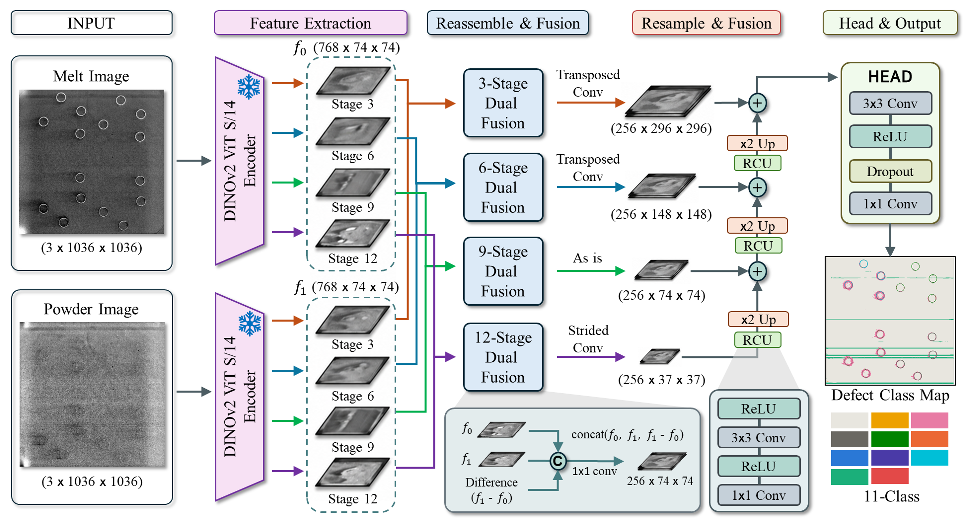
\includegraphics[width=\linewidth]{Figs/DefectSegAM_Architecture.pdf}
\caption{DefectSegAM 아키텍처 개요. 각 레이어의 Melt 이미지 $I_0$와
Powder 이미지 $I_1$은 register token을 포함한 단일 동결 DINOv2
ViT-B/14 인코더(86\,M 파라미터, 가중치 공유 이중 forward)를 통과한다.
트랜스포머 블록 3, 6, 9, 12 이후에서 추출된 특징 맵은 단계별로
$\left[\mathbf{F}^{(0)}_s;\, \mathbf{F}^{(1)}_s;\,
\mathbf{F}^{(1)}_s - \mathbf{F}^{(0)}_s\right]$의
채널 방향 결합(channel-wise concatenation)과 단계별 $1 \times 1$
projection을 통해 256채널로 융합되고, DPT-style reassemble/top-down
융합 디코더(헤드를 포함해 14.6\,M 학습 파라미터)로 디코딩되며,
합성곱 헤드가 산출한 11개 클래스 logit은 bilinear upsampling을 통해
입력 해상도로 복원된다.}
\label{fig:architecture}
\end{figure}

% -------------------------------------------------------------------------
\subsection{문제 설정과 실험용 11-클래스 결함 온톨로지}
\label{sec:method-problem}

Powder bed fusion 공정에서 각 적층 레이어는 두 장의 가시광 카메라
이미지로 기록된다. 하나는 용융(melting) 단계 직후에 촬영되는
\emph{Melt 이미지} $I_0$이고, 다른 하나는 이어지는 분말 도포
(recoating) 단계 이후에 촬영되는 \emph{Powder 이미지} $I_1$이다. 두
뷰는 상호 보완적인 증거를 담고 있으며, DSCNN도 한 레이어의 두 이미지를
함께 입력으로 사용한다~\cite{Scime2020DSCNN}. 개략적으로 정리하면 Recoater
Hopping, Recoater Streaking, Incomplete Spreading, 흩어진 Debris와 같은
도포 관련 이상은 주로 Powder 이미지에서 관찰되는 반면, Spatter, Over
Melting, Under Melting과 같은 용융 관련 이상은 Melt 이미지에 나타나며,
Swelling과 Super-Elevation은 두 이미지 모두에서 드러난다. 이 구분은
저자들의 정리이며, 각 결함이 어느 이미지에서 관찰되는지는
\S\ref{sec:method-taxonomy}에서 외형 기준으로 다시 정리한다. 따라서
DefectSegAM은 이미지 쌍 $(I_0, I_1)$을 입력으로 받아, powder bed의 각
픽셀을 11개 클래스 중 하나에 할당하는 조밀한(dense) 의미 분할(semantic segmentation) 라벨맵
$\hat{M} \in \{0,\dots,10\}^{H \times W}$을 예측한다.

표~\ref{tab:classes}에 정리한 온톨로지는 ORNL Peregrine 플랫폼의
12-클래스 라벨 공간~\cite{Scime2020DSCNN,ORNL_CoRegistered_Dataset}으로부터 유도되며, 이
라벨 공간은 두 개의 비결함 클래스 \emph{Powder}와 \emph{Printed}에 열
개의 이상(anomaly) 클래스를 더한 구성이다. DefectSegAM은 원본 12개
클래스 중 11개를 일대일 매핑으로 유지한다(원본 식별자 0--8은 동일하게
매핑되고, 원본 \emph{Over Melting} 10과 \emph{Under Melting} 11은 각각
9와 10으로 매핑된다). 유일하게 제외되는 클래스는 원본 클래스~9인
\emph{Misprint}(의도된 파트 형상 밖에 프린팅된 재료)이다. Misprint는
베드의 외관이 아니라 CAD 의도를 기준으로 정의되는 클래스이므로,
ignore index $-1$을 할당하여 손실과 모든 평가 지표에서 제외한다.
미세조정 단계에서는 이 온톨로지에 대응 클래스가 없는 다중 장비 GT
코퍼스의 소스 고유(native) 클래스들 역시 동일한 ignore index로
흡수된다(\S\ref{sec:method-training}). 이 온톨로지는 본 논문의 모든
실험이 사용하는 클래스 공간이다. 그 용어가 물려받은 원인 기준과 외형
기준의 혼재, 그리고 이를 정리한 외형 기준 분류 체계는
\S\ref{sec:method-taxonomy}에서 다룬다.

표~\ref{tab:classes}에는 또한 다섯 개의 ORNL 빌드 B1.1--B1.5
전체(Stage-1 학습 \emph{및} 검증; \S\ref{sec:setup}의 필터링된 레이어
집합에 대해 $1036 \times 1036$ 모델 해상도에서 집계)에 대한 재매핑 후
클래스별 총 픽셀 수를 함께 보고한다. 이 분포는 극단적인
long-tail 형태를 보인다. 가장 빈번한 클래스(Powder,
$1.533 \times 10^{10}$ 픽셀)와 가장 희소한 결함 클래스(Recoater
Hopping, 25 픽셀) 사이의 비율은 거의 아홉 자릿수(nine orders of
magnitude)에 이르며, 여러 결함 클래스가 추가로 단일 빌드에 집중되어
있다(예: Over Melting 픽셀의 99.8\,\%와 Under Melting 픽셀의
99.9\,\%는 빌드 B1.2에서, Super-Elevation 픽셀의 98\,\%는 빌드
B1.5에서 발생한다). 이러한 불균형이
\S\ref{sec:method-imbalance}의 샘플링, 증강, 손실 설계의 직접적인
동기가 된다.

\begin{table}[t]
\centering
\caption{DefectSegAM의 11-클래스 온톨로지와 ORNL Peregrine 원본
12-클래스 라벨 공간~\cite{Scime2020DSCNN,ORNL_CoRegistered_Dataset}으로부터의 매핑. 원본
클래스 0--8은 일대일로 매핑되고, 원본 Over Melting(10)과 Under
Melting(11)은 DefectSegAM 식별자 9와 10으로 매핑되며, 유일하게
무시되는 원본 클래스는 Misprint(9)로서 ignore index $-1$에 매핑되어
손실과 평가에서 제외된다. 픽셀 수는 다섯 개의 ORNL Co-Registered 빌드
B1.1--B1.5 전체(\S\ref{sec:setup}의 레이어 필터링을 거친 Stage-1 학습
및 검증 레이어, $1036 \times 1036$ 모델 해상도)에 대한 재매핑 후
총계이다. 설명 열은 ORNL 원 정의를 따른 것이며, 같은 결함을 외형
기준으로 다시 정의한 특징은 표~\ref{tab:taxonomy}에 제시한다.}
\label{tab:classes}
\small
\begin{tabular}{clcp{5.6cm}r}
\toprule
ID & Class & ORNL ID & 설명 & 픽셀 수 (B1.1--B1.5) \\
\midrule
0  & Powder               & 0  & 용융되지 않은 분말 베드 & $1.533 \times 10^{10}$ \\
1  & Printed              & 1  & 용융(프린팅)된 재료 & $7.05 \times 10^{8}$ \\
2  & Recoater Hopping     & 2  & 리코터가 표면 아래의 파트에 부딪혀 발생하는 물결 무늬 & $25$ \\
3  & Recoater Streaking   & 3  & 손상된 리코터 블레이드 또는 끌려간 입자로 인한 줄무늬 & $1.87 \times 10^{8}$ \\
4  & Incomplete Spreading & 4  & 분말 도포량 부족 & $8.67 \times 10^{5}$ \\
5  & Swelling             & 5  & 분말 평면 위로 변형되거나 뒤틀린 프린팅 재료 & $1.0 \times 10^{7}$ \\
6  & Debris               & 6  & 중소 규모 분말 베드 교란을 포괄하는 catch-all 클래스 & $1.8 \times 10^{6}$ \\
7  & Super-Elevation      & 7  & 프린팅 영역 위의 분말 피복 부족 & $2.68 \times 10^{5}$ \\
8  & Spatter              & 8  & 베드 위에 침적된 용융 풀 방출물 & $6.67 \times 10^{8}$ \\
9  & Over Melting         & 10 & 과도한 에너지 밀도로 용융된 영역 & $3.94 \times 10^{5}$ \\
10 & Under Melting        & 11 & 불충분한 에너지 밀도로 용융된 영역 & $2.8 \times 10^{7}$ \\
\midrule
$-1$ (무시됨) & Misprint & 9  & 의도된 파트 형상 밖의 프린팅 재료 & --- \\
\bottomrule
\end{tabular}
\end{table}

% -------------------------------------------------------------------------
\subsection{외형 기준 결함 분류 체계(제안; 실험 미적용)}
\label{sec:method-taxonomy}

표~\ref{tab:classes}의 온톨로지가 물려받은 용어는 판정 기준이 클래스마다
다르다. Over Melting과 Under Melting은 에너지 밀도라는 원인으로,
Misprint는 CAD 의도로 정의되는 반면, 나머지 결함도 상당수는 외형과
원인을 섞어 정의된다. 예컨대 Peregrine v2021-03 릴리스의 정의는
Swelling과 Super-Elevation을 모두 파트가 분말 베드 위로 솟은 외형으로
기술하면서, Swelling은 과도한 국소 에너지 입력, Super-Elevation은 분말
피복 부족 또는 잔류 응력에 의한 뒤틀림의 결과로 원인 절에서만
구분한다~\cite{Peregrine_v2021_03}. 반면 본 논문 라벨의 출처인 ORNL
정의(표~\ref{tab:classes})는 두 클래스를 각각 분말 평면 위로 변형된
프린팅 재료와 프린팅 영역 위의 분말 피복 부족으로 기술하므로, 같은
클래스라도 릴리스마다 판정 기준이 다르다. 저자들의 관찰로는 두 클래스가
이미지에서 모두 파트가 분말 위로 솟은 유사한 형상으로 나타나 구별하기
어렵다. ASTM E3353-22 표준 지침~\cite{ASTME3353}의 공개된 4절도 분말층
이상을 리코팅 오류와 파트 형성 오류라는 원인 범주로 나눌 뿐, skipping과
insufficient powder delivery의 레이어 이미지 외형 차이는 제시하지
않는다(레이어 이미지에서의 상세 기술은 본 연구가 검토하지 못한 8절로
미룬다). 또한 ORNL 12-클래스 공간과 본 연구가 검토한 사람 주석 코퍼스의
클래스 목록에는 둘을 나누는 클래스가 없다. 분말 도포 부족은 L-PBF
소스에서 Incomplete Spreading 하나로만 정의되므로(binder-jet 소스에서는
같은 정의의 Short Feed)~\cite{ORNL_CoRegistered_Dataset,Peregrine_v2021_03,Peregrine_v2022_10},
어느 코퍼스도 둘을 구분하여 주석하지 않는다. 픽셀 단위
주석은 이미지만 보고 수행되므로, 이미지에서 구분할 수 없는 기준은 주석자
간 불일치와 라벨 노이즈로 이어진다. 분말 베드 이미지의 외형으로 이상을
검출·분류한다는 접근 자체는 Scime와 Beuth~\cite{Scime2018Anomaly}와
DSCNN~\cite{Scime2020DSCNN}이 이미 취한 것이지만, 그 클래스 정의는 위와
같이 원인과 CAD 의도를 포함한다. 본 연구는 그 원칙을 명시적 규칙으로
확장한다. 즉 데이터셋 정의에 이미 들어 있는 방향 기준(Recoater
Hopping과 Recoater Streaking을 리코팅 방향에 수직·평행한 줄무늬로
정의~\cite{Peregrine_v2021_03,Peregrine_v2022_10})과 영역 기준(ORNL의
Spatter 정의, v2022-10 릴리스의 ``Spatter on
Powder''~\cite{Peregrine_v2022_10}, 그리고 \S\ref{sec:method-inference}의
후처리 규칙 2)을 판별 규칙으로 정리하고, 원인 또는 CAD 기준으로 정의된
클래스를 재정의하거나 제외하며, 외형이 유사하여 구별하기 어려운 클래스를
통합하여, 결함을 \emph{레이어 이미지에 나타난 특징}을 판정 기준으로
정의하는(위치 판정에는 파트 마스크를 보조로 사용하는) 외형
기준(appearance-based) 결함 분류 체계를 제안한다. 이 체계는 결함 여덟
종에 배경 두 종(Powder, Printed)을 더한 10개 클래스로 구성되며(Under
Melting을 외형 기준으로 재정의하여 유지할 경우 결함 아홉 종이 된다;
아래 (v) 참조), 각 클래스가 관찰되는 이미지(도포 직후의 Powder 이미지
$I_1$, 용융 직후의 Melt 이미지 $I_0$, 또는 둘 다), 이미지에 나타난
특징, 그리고 ORNL 12-클래스 공간 및 ASTM E3353-22 어휘와의 대응을
표~\ref{tab:taxonomy}에 정리하였다. 이미지 열은 저자들의 관찰에 따른
것이다. \TODO{이미지 열의 관찰 근거(검토한 소스·레이어 수)를 명시할
것.}

제안 체계의 결함 클래스 여덟 종의 예시 사진을 여덟 장의 그림에 나누어
보인다. 각 패널 아래에는 클래스명과 원자료의 빌드·레이어 표기를
적었으며, 표기의 M160과 M280은 원자료의 장비 표기를 그대로 옮긴
것이다. 어두운 사진에서도 결함이 보이도록 사진에는 자르기(crop) 외에
화면 전체에 균일한 레벨·감마 조정(levels and gamma adjustment)을
적용하였으며, 그 세부와 표시 방식은 그림~\ref{fig:examples-is-rh}의
캡션에 적었다. 그림~\ref{fig:examples-is-rh}(a)--(c)는 Incomplete
Spreading으로, 분말이 고르게 덮인 영역과 그렇지 않은 영역의 경계(이하
도포 경계)를 점선으로 표시하였다. (a)에서는 도포 경계가 베드 위쪽에서
불규칙하게 내려오고, (b)에서는 왼쪽과 오른쪽에 호 모양의 도포 경계가
하나씩 있으며, (c)에서는 왼쪽에 사선 방향의 도포 경계가 있다. (c)의 흰
상자 두 곳은 원자료가 Over Melting으로 표시한, 표면이 거뭇하게 변색된
파트이다. (d)는 Recoater Hopping으로, 시편 배열의 둘째 행과 셋째 행을
가로질러 가로 띠가 반복된다. 그림~\ref{fig:examples-pc}의 네 장은 같은
빌드에서 촬영된 Powder Collapse이다. 레이어 1323의 (a)에서는 베드
아래쪽 가장자리의 분말이 함몰되어 있고(확대 인셋), 레이어 1455의
(b)에서는 오른쪽 가장자리에 길쭉한 함몰 두 곳이, 레이어 1531의
(c)에서는 오른쪽 가장자리의 함몰과 베드 중앙의 원형 함몰이 보인다.
원자료에 레이어 번호가 없는 (d)에서는 중앙의 함몰이 (c)보다 크고,
오른쪽 가장자리의 함몰도 보인다. 저자들의 관찰로는 이 빌드에서 파트가
움직이면서 분말이 무너졌으며, 파트가 없는 분말을 레이저가 조사하여 생긴
흔적을 Over Melting으로 볼지는 정하지 못하였다. \TODO{(d)의 레이어
번호를 확인하고, 파트 이탈 뒤 분말만 조사된 영역의 클래스(Over Melting
여부)를 확정할 것.}

그림~\ref{fig:examples-rs1} 및
그림~\ref{fig:examples-rs2}의 여덟 장은 Recoater Streaking이다.
그림~\ref{fig:examples-rs1}(a)에는 세로 줄무늬 세 줄이 있다. (b)는
줄무늬가 매우 희미하여, 분말 픽셀의 열 방향 평균 밝기가 주변보다 낮은
두 위치만 표시하였다. (c)에는 분말 위로 드러난 파트를 지나는 굵은 세로
줄무늬 한 줄이 있고, (d)의 줄무늬는 넓은 띠로 발달해 있다(기울어진
상자). 그림~\ref{fig:examples-rs2}(a)는 희미하고 가는 세로 줄무늬
묶음, (b)는 뚜렷한 세로 줄무늬 한 줄과 희미한 한 줄, (c)는 시편을
지나는 세로 줄무늬 세 줄, (d)는 베드 왼쪽에 조밀하게 반복되는 세로
줄무늬이다. 제안 체계의 판별 규칙에서 Recoater Streaking은 리코팅
방향과 평행한 줄무늬, Recoater Hopping은 리코팅 방향과 수직인 반복
줄무늬이지만, 사진의 실제 리코팅 방향은 확인하지 못하였으므로
그림~\ref{fig:examples-rs1} 및 그림~\ref{fig:examples-rs2}의 세로
줄무늬와 그림~\ref{fig:examples-is-rh}(d)의 가로 띠에 대한 클래스
판정은 원자료의 분류에 따른 것이다.

그림~\ref{fig:examples-se1}의 네 장과
그림~\ref{fig:examples-se2-sp}(a)--(c)는 Super Elevation이다.
그림~\ref{fig:examples-se1}(a)에서는 긴 막대형 파트가 분말 위로 드러나
있고, 흰 상자는 원자료가 Over Melting으로 표시한 막대 끝의 밝은
부분이다. (b)에서는 사선 방향 파트의 가장자리 일곱 곳이 분말 위로
드러나 있으며(확대 인셋), 흰 상자는 세로 줄무늬(Recoater
Streaking)이다. (c)에서는 파트 끝이 분말 위로 드러나 있고(확대 인셋),
흰 점선은 도포 경계(Incomplete Spreading)이다. (d)에서는 긴 파트의
가장자리가 솟아 어두운 선으로 보이며, 흰 상자 두 곳은 세로 줄무늬이다.
그림~\ref{fig:examples-se2-sp}(a)에서는 시편 아홉 개의 앞쪽 가장자리가
분말 위로 드러나 있는데(확대 인셋), 저자들은 시편이 반짝이는 것으로
보아 Powder Collapse가 있었을 것으로 추정한다. (b)에서는 빗살 모양
파트의 살 끝이 솟아 변색되어 있다. (c)에는 Super Elevation(시편 세
줄)과 Spatter(시편 왼쪽 분말 영역에 흩어진 검은 입자, 세 곳)가 함께
나타나며, 두 클래스가 모두 이 그림의 대상이므로 둘 다 붉은색으로
표시하고 약어 태그(SE, SP)로 구분하였다. (d)는 Spatter로, 오른쪽 위
시편 세 개의 왼쪽 분말 영역이 어둡게 보인다.

그림~\ref{fig:examples-om}(a)--(c)는 Over Melting이고, (d)는 (c)의
붉은 상자를 확대한 것이다. (a)에서는 고리 모양 파트의 안쪽 표면 두
곳이 거뭇하게 변색되어 있다. (b)에서는 막대형 파트의 표면이 검게
변색되어 있으며(기울어진 상자), 흰 상자는 분말 위로 드러난 파트(Super
Elevation)이다. (c)에서는 $5 \times 5$ 시편 배열의 오른쪽 위 네 시편이
거뭇하게 변색되어 있다. 이와 같이 어둡게 보이는 외형은 외형 기준의
판정 근거일 뿐, 그 자체가 해당 파트의 규격 이탈(out of
specification)을 뜻하지는 않는다.
그림~\ref{fig:examples-db}(a)--(c)는 Debris이고, (d)는 (a)의
확대이다. (a)의 붉은 상자는 분말 면의 검은 덩어리이고, 흰 상자는 분말
위로 드러난 파트(Super Elevation)이다. 저자들의 관찰로는 이 사진에서
Debris와 Super Elevation을 구별하기 어려웠으며, 이는 제안 체계의 판별
규칙이 지닌 한계를 보여 주는 사례이다. (b)와 (c)는 같은 빌드의 레이어
86과 88로, 제자리에서 밀려나 분말 면에 놓인 파트 조각이 각각 두 곳
보인다. (c)의 위쪽에는 리코터가 보이며, 저자들의 관찰로는 밀려난
조각이 끝내 리코터에 걸렸다. 이 체계는 차기 주석과 학습을 위한
제안이며, 본 논문의 모든 학습과 평가는 표~\ref{tab:classes}의 11-클래스
온톨로지로 수행되었다.

\begin{table}[t]
\centering
\caption{제안하는(본 논문의 실험에는 사용하지 않은) 외형 기준 결함 분류
체계(결함 8종 + 배경 2종)와 기존 어휘의 대응. 이미지 열은 결함이 나타나는
이미지를 뜻한다($I_1$ = 분말 도포 직후의 Powder 이미지, $I_0$ = 용융
직후의 Melt 이미지, 둘 다 = 두 이미지 모두). ORNL 열은
표~\ref{tab:classes}의 원본 12-클래스 식별자이고, ASTM 열은 ASTM
E3353-22~\cite{ASTME3353}의 이상 용어를 저자들이 대응시킨 것이며, 괄호
안의 영역 구분은 표준이 아니라 본 체계의 판별 규칙에 따른 것이다.}
\label{tab:taxonomy}
\small
\setlength{\tabcolsep}{4pt}
\begin{tabularx}{\textwidth}{@{}>{\raggedright\arraybackslash}p{2.3cm}c>{\raggedright\arraybackslash}X>{\raggedright\arraybackslash}p{2.2cm}>{\raggedright\arraybackslash}p{2.7cm}@{}}
\toprule
클래스 & 이미지 & 이미지에 나타난 특징 & ORNL 12-클래스 & ASTM E3353-22 \\
\midrule
\multicolumn{5}{@{}l}{\emph{배경}} \\
Powder  & --- & 결함도 파트도 없는 분말 베드 & Powder (0) & --- \\
Printed & --- & 결함이 없는 프린팅 영역 & Printed (1) & --- \\
\multicolumn{5}{@{}l}{\emph{결함}} \\
Incomplete Spreading & $I_1$ & 분말 영역에 남는 얕고 미세한 미도포 자국 & Incomplete Spreading (4) & Skipping; Insufficient powder delivery \\
Powder Collapse      & 둘 다 & 분말이 산사태처럼 무너져 내린 큰 형상 & --- (신규) & Skipping; Insufficient powder delivery \\
Recoater Streaking   & 둘 다 & 리코팅 방향과 평행한 줄무늬 & Recoater Streaking (3) & Scraping \\
Recoater Hopping     & 둘 다 & 리코팅 방향과 수직인 반복 줄무늬 & Recoater Hopping (2) & Part strike \\
Super Elevation      & $I_1$ & 파트가 분말 위로 돌출된 형상 & Swelling (5); Super-Elevation (7) & Distortion; Superelevation; Humping (잠정) \\
Spatter              & $I_0$ & 분말 영역에 재가 날린 것처럼 보이는 거뭇한 영역 & Spatter (8) & Excessive spatter/ejecta (분말 영역) \\
Over Melting         & $I_0$ & 파트 영역 위에 거뭇하게 재가 보이는 영역 & Over Melting (10; 재검토) & Overheating\slash Overmelting; Excessive spatter/ejecta (파트 영역) \\
Debris               & 둘 다 & 분말 면에 포착된 불규칙한 덩어리나 조각 & Debris (6) & --- \\
\midrule
(제외) & --- & CAD 의도 기준 클래스 & Misprint (9) & --- \\
(미결) & --- & 공정 파라미터 기준 클래스; 처리 미결(본문 참조) & Under Melting (11) & --- \\
\bottomrule
\multicolumn{5}{@{}p{\textwidth}@{}}{\footnotesize 이미지 열은 저자들의 관찰에 따른 것으로(Powder
Collapse는 두 코퍼스에 라벨된 사례가 없어 신규 주석 시 확인이 필요하다),
\S\ref{sec:method-problem}의 개략적 구분과는 Swelling/Super-Elevation(둘 다 $\rightarrow$ $I_1$)과
Recoater Streaking, Recoater Hopping, Debris($I_1$ $\rightarrow$ 둘 다)에서 차이가 있다.
특징 열에는 시각 특징만 적었으며, 통상적 원인은 판정 기준이 아니다.
배경 행의 이미지 열 ``---''는 결함이 아니므로 구분이 해당 없음을, 그 밖의 ``---''는 대응 용어가
없음을 뜻한다.
Swelling과 Super-Elevation을 통합한 클래스는 11-클래스 온톨로지의 Super-Elevation과 구별하기
위해 하이픈 없이 Super Elevation으로 표기하고, ASTM 열의 Superelevation은 표준 원문의 철자이다.
표준의 공개된 4절은 humping을 파트 형성 오류로 들면서 과열의 징후로도 들므로, Humping의
Super Elevation 대응은 트랙 융기의 레이어 이미지 외형을 확인하기 전까지 잠정적이다.
Over Melting의 ORNL 라벨 재매핑에는 재검토가 필요하다(본문 참조).}
\end{tabularx}
\end{table}

\begin{figure}[p]
\centering
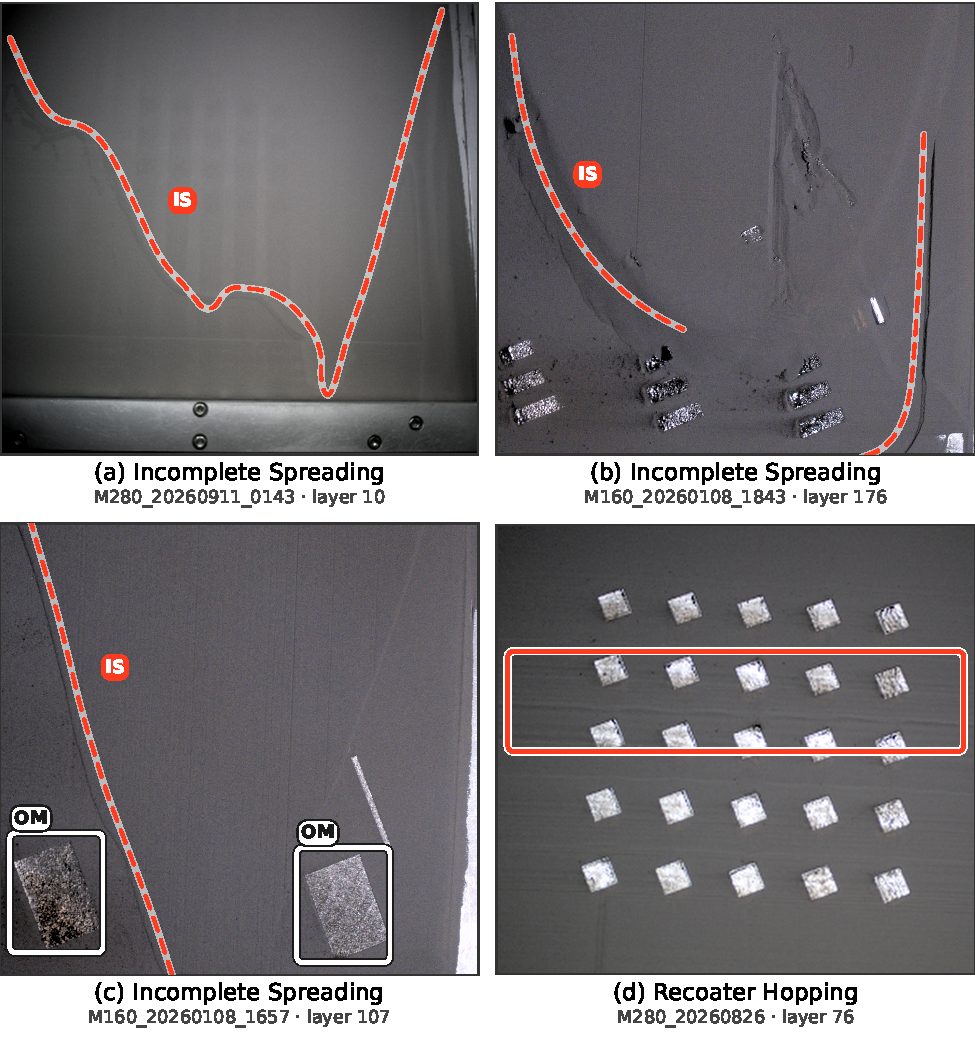
\includegraphics[width=\linewidth,height=0.80\textheight,keepaspectratio]{Figs/Defect_Examples_IS_RH.pdf}
\caption{제안하는 외형 기준 결함 분류 체계(표~\ref{tab:taxonomy})의
예시 사진. (a)--(c) Incomplete Spreading(IS); (d) Recoater Hopping.
저자들이 넣은 표시 중 붉은 것은 해당 그림이 다루는 클래스, 흰 것은
함께 나타난 다른 클래스이고(약어 태그로 구분; OM = Over Melting),
상자는 결함 위치, 점선은 도포 경계 옆에 비켜 그린 안내선, 인셋의
숫자는 확대 배율이다. 사진 처리는 자르기와 사진별로 화면 전체에
균일하게 적용한 레벨·감마 조정뿐이다. 이 조정은 휘도(luminance)
기준이고 선형 증폭은 2.6배 이하, 감마 지수는 0.5--1.0이며, 국소 보정과
합성은 하지 않았다. \TODO{사진의 출처(장비 M160·M280의 정식 명칭,
재료, 카메라)와 사용 허가를 명시할 것.}}
\label{fig:examples-is-rh}
\end{figure}

\begin{figure}[p]
\centering
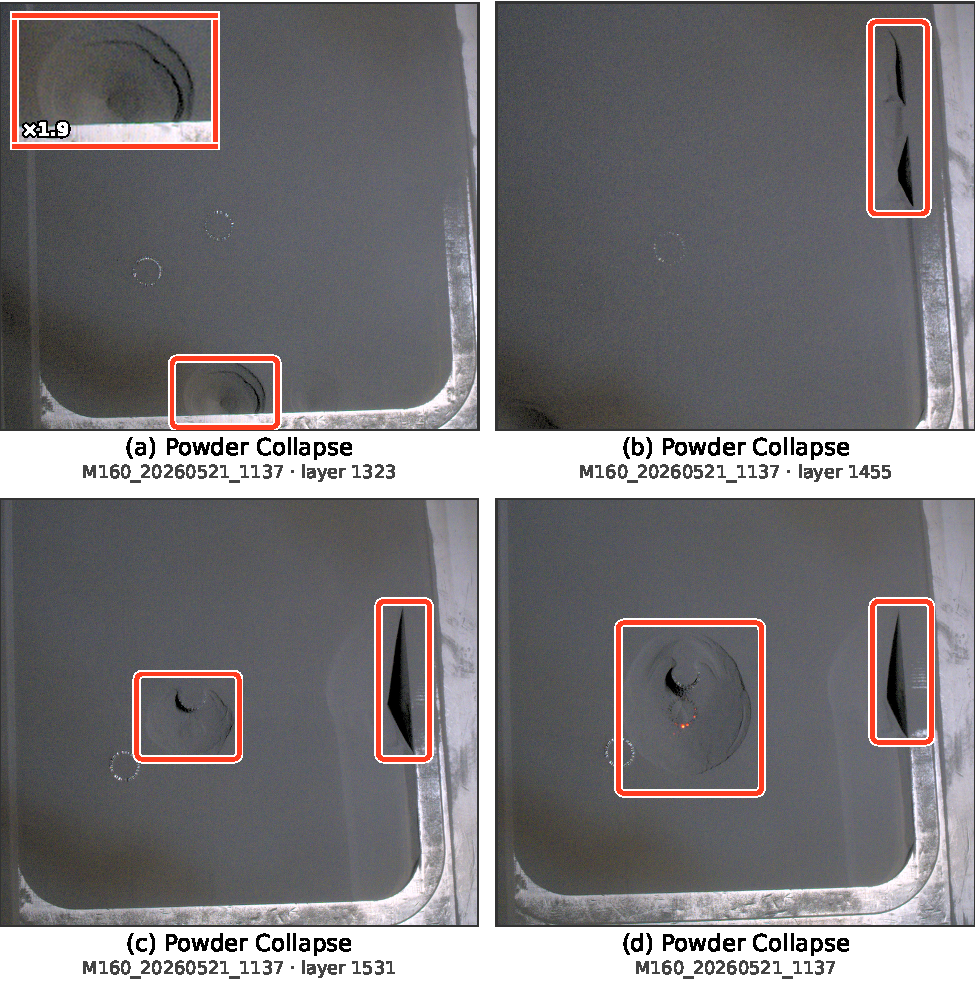
\includegraphics[width=\linewidth,height=0.80\textheight,keepaspectratio]{Figs/Defect_Examples_PC.pdf}
\caption{제안 체계(표~\ref{tab:taxonomy})의 Powder Collapse 예시 사진.
(a)--(d) 같은 빌드에서 촬영된 Powder Collapse. 표시 방식과 사진 처리는
그림~\ref{fig:examples-is-rh}와 같다.}
\label{fig:examples-pc}
\end{figure}

\begin{figure}[p]
\centering
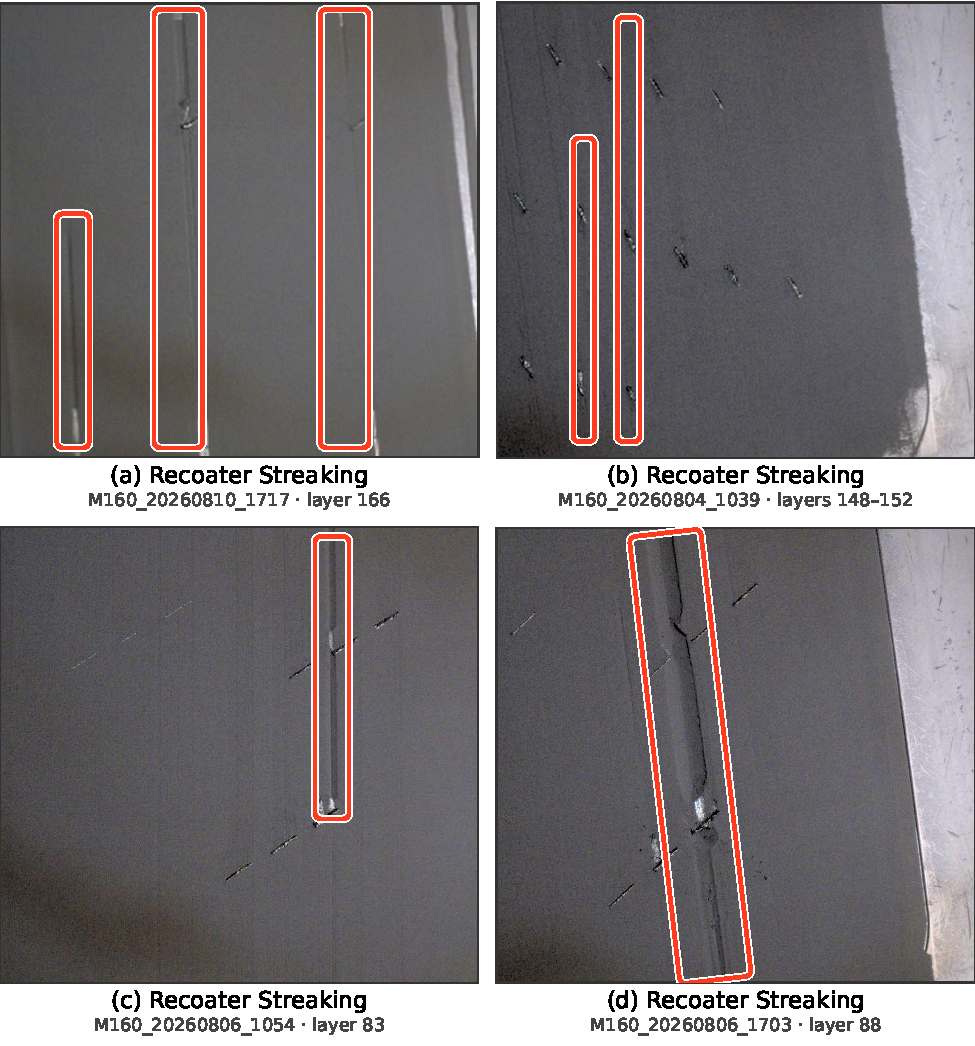
\includegraphics[width=\linewidth,height=0.80\textheight,keepaspectratio]{Figs/Defect_Examples_RS1.pdf}
\caption{제안 체계(표~\ref{tab:taxonomy})의 Recoater Streaking 예시
사진(여덟 장 중 첫 네 장). (a)--(d) Recoater Streaking. 표시 방식과
사진 처리는 그림~\ref{fig:examples-is-rh}와 같다.}
\label{fig:examples-rs1}
\end{figure}

\begin{figure}[p]
\centering
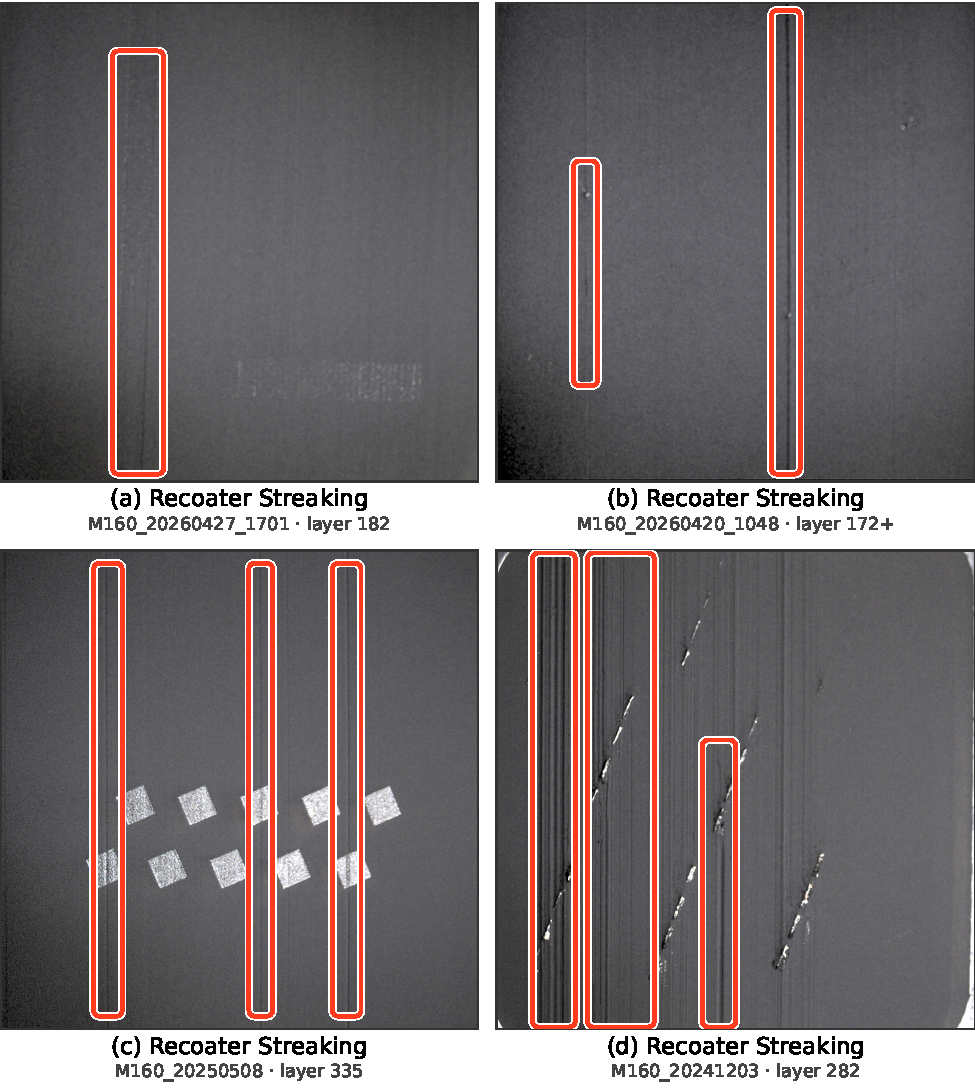
\includegraphics[width=\linewidth,height=0.80\textheight,keepaspectratio]{Figs/Defect_Examples_RS2.pdf}
\caption{제안 체계(표~\ref{tab:taxonomy})의 Recoater Streaking 예시
사진(여덟 장 중 나머지 네 장). (a)--(d) Recoater Streaking. 표시
방식과 사진 처리는 그림~\ref{fig:examples-is-rh}와 같다.}
\label{fig:examples-rs2}
\end{figure}

\begin{figure}[p]
\centering
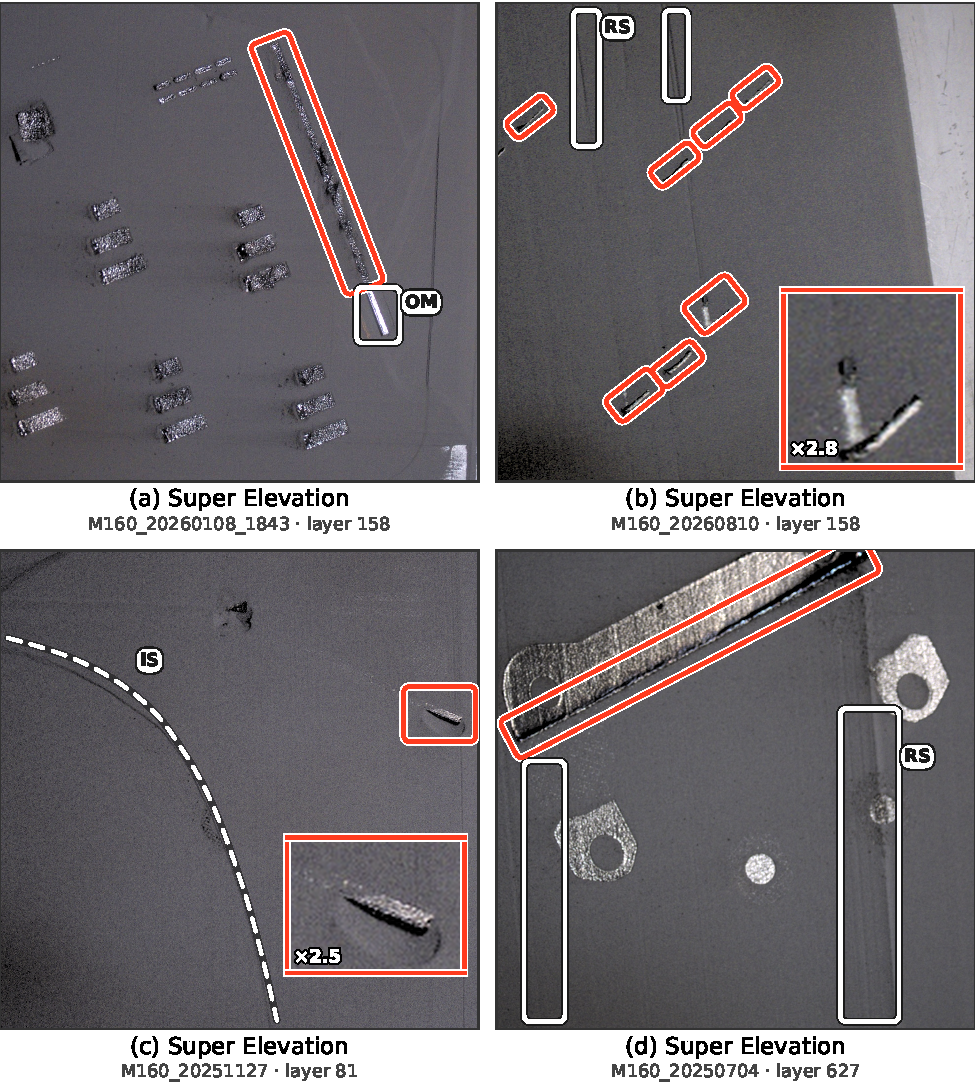
\includegraphics[width=\linewidth,height=0.80\textheight,keepaspectratio]{Figs/Defect_Examples_SE1.pdf}
\caption{제안 체계(표~\ref{tab:taxonomy})의 Super Elevation 예시 사진.
(a)--(d) Super Elevation. 흰 표시는 함께 나타난 Over Melting(OM; (a)),
Recoater Streaking(RS; (b), (d)), Incomplete Spreading(IS; (c)의
점선)이다. 표시 방식과 사진 처리는 그림~\ref{fig:examples-is-rh}와
같다.}
\label{fig:examples-se1}
\end{figure}

\begin{figure}[p]
\centering
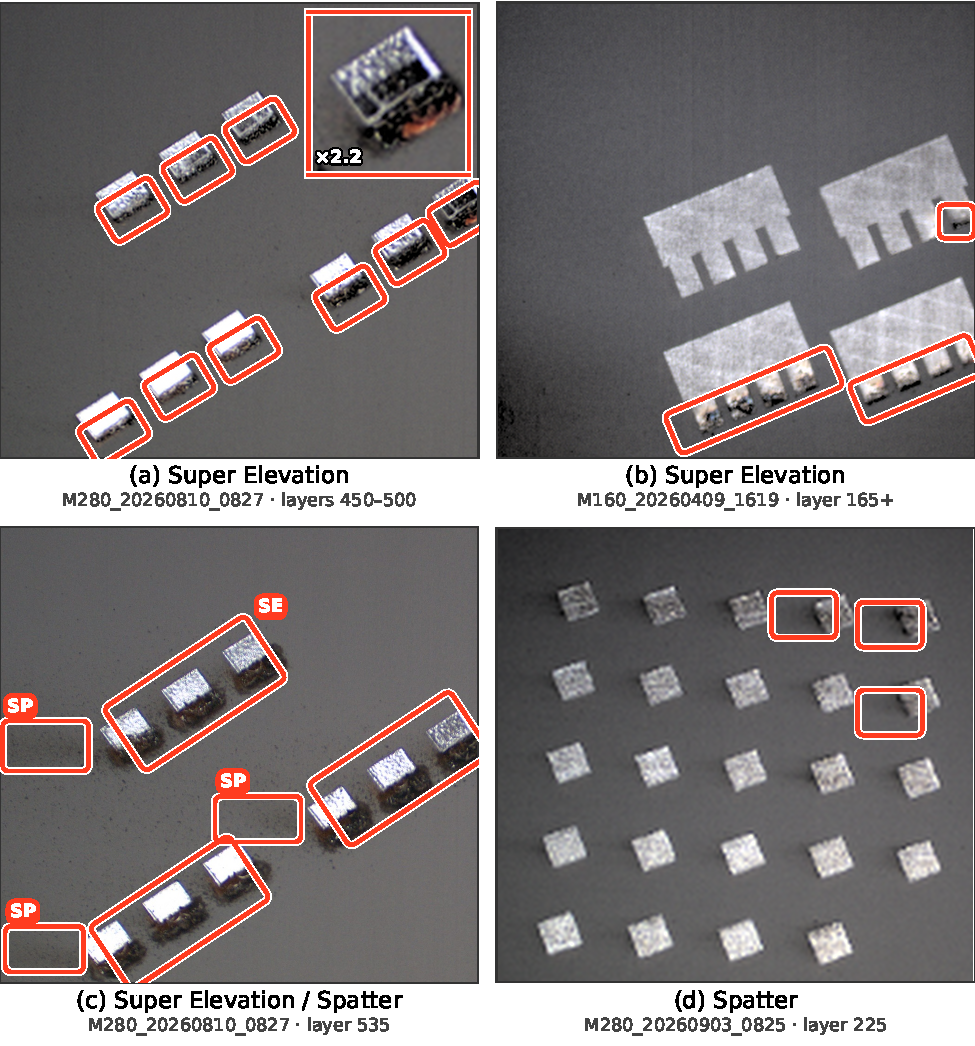
\includegraphics[width=\linewidth,height=0.80\textheight,keepaspectratio]{Figs/Defect_Examples_SE2_SP.pdf}
\caption{제안 체계(표~\ref{tab:taxonomy})의 Super Elevation과 Spatter
예시 사진. (a), (b) Super Elevation; (c) Super Elevation(SE)과
Spatter(SP); (d) Spatter. (c)에서는 두 클래스가 모두 이 그림의
대상이므로 둘 다 붉은색으로 표시하였다. 표시 방식과 사진 처리는
그림~\ref{fig:examples-is-rh}와 같다.}
\label{fig:examples-se2-sp}
\end{figure}

\begin{figure}[p]
\centering
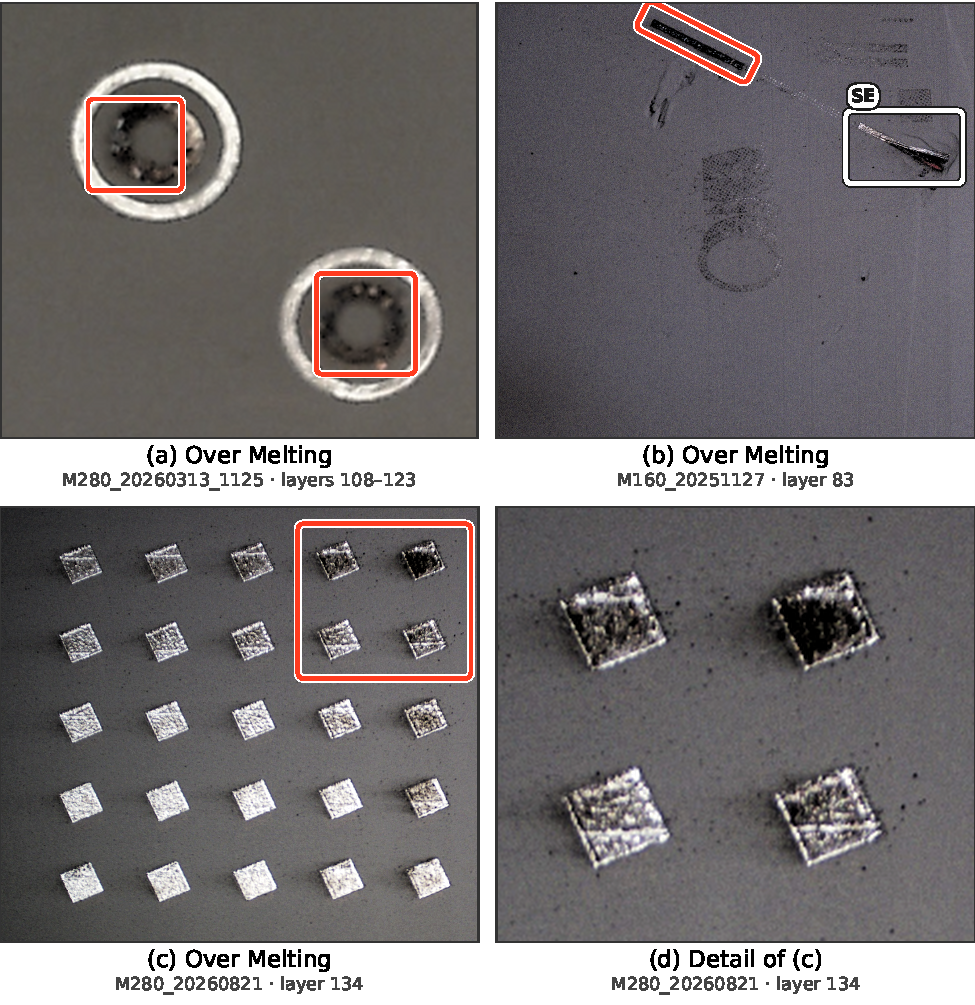
\includegraphics[width=\linewidth,height=0.80\textheight,keepaspectratio]{Figs/Defect_Examples_OM.pdf}
\caption{제안 체계(표~\ref{tab:taxonomy})의 Over Melting 예시 사진.
(a)--(c) Over Melting; (d) (c)의 붉은 상자 영역 확대. (b)의 흰 상자는
함께 나타난 Super Elevation(SE)이다. 표시 방식과 사진 처리는
그림~\ref{fig:examples-is-rh}와 같다.}
\label{fig:examples-om}
\end{figure}

\begin{figure}[p]
\centering
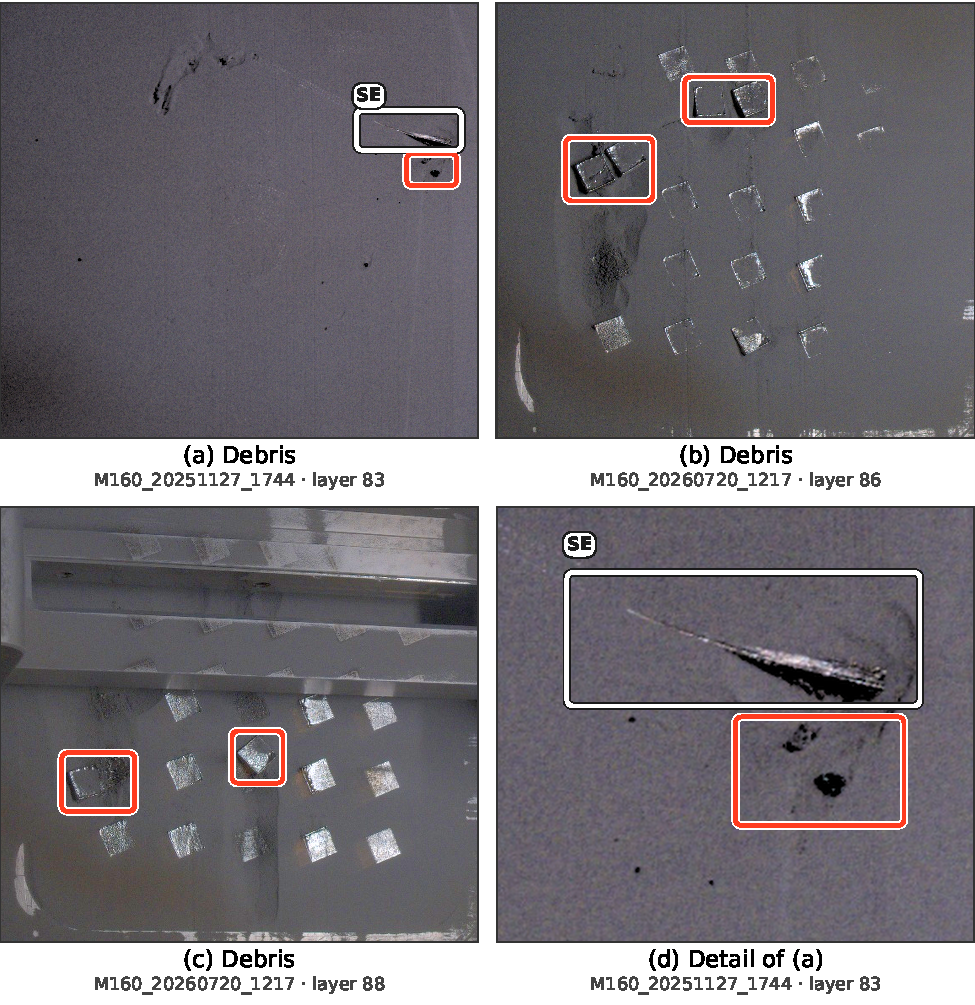
\includegraphics[width=\linewidth,height=0.80\textheight,keepaspectratio]{Figs/Defect_Examples_DB.pdf}
\caption{제안 체계(표~\ref{tab:taxonomy})의 Debris 예시 사진. (a)--(c)
Debris; (d) (a)의 확대. (a)와 (d)의 흰 상자는 함께 나타난 Super
Elevation(SE)이다. 표시 방식과 사진 처리는
그림~\ref{fig:examples-is-rh}와 같다.}
\label{fig:examples-db}
\end{figure}

11-클래스 온톨로지와 비교하면 제안 체계의 변경은 다섯 가지이다. (i)
Swelling과 Super-Elevation은 모두 파트가 분말 위로 솟은 유사한
형상이어서 이미지만으로 구별하기 어려우므로 하나의 Super
Elevation(11-클래스의 Super-Elevation과 구별하기 위해 하이픈 없이
표기한 통합 클래스)으로 통합한다. 면적 기준으로 파트 가장자리의 소규모
융기(Edge Swelling)를 하위 클래스로 분리하는 방안은 임계값을 정한 뒤
검토한다. (ii) 제안 체계는 Spatter와 Over Melting을 모두 거뭇한
영역이라는 외형으로 정의하고(저자들의 관찰로는 두 결함이 유사하게
거뭇하게 나타난다) 위치로만 구분하여, 파트 마스크를 기준으로 분말
영역의 거뭇한 픽셀은 Spatter, 파트 영역의 거뭇한 픽셀은 Over Melting으로
판정한다. 두 클래스를 하나로 합치고 파트 마스크로 후처리 분할하는
대안도 가능하지만, 파트 마스크가 없는 소스(아래 둘째 규칙의 한계)와
실시간 배포에서는 모델이 Printed 영역을 이미지에서 직접 추론해야 하므로
두 클래스를 유지한다. 따라서 두 클래스의 라벨 정의는 파트 마스크에
의존하며, 모델은 파트 영역과 분말 영역의 구분을 이미지에서 학습해야
한다.
(iii) 분말이 무너져 내린 형상은 Incomplete Spreading과 원인(분말
부족)이 일부 겹칠 수 있으나(저자들은 빌드플레이트 패드 마모도 원인으로
추정한다) 이미지 특징이 크게 다르므로 Powder Collapse를 신설한다. (iv)
Misprint는 CAD 의도 기준 클래스이므로 계속 제외한다. 제안 체계도 파트
마스크를 사용하지만, Misprint는 CAD 의도 자체가 판정 기준인 반면 파트
마스크는 위치 정보로만 쓰인다. (v) Under Melting은 저에너지
밀도라는 공정 파라미터로 정의되어 외형 기준 원칙에 어긋난다. Over
Melting을 파트 영역 위의 거뭇한 영역이라는 외형으로 재정의한 것과 달리
Under Melting은 재정의하지 않았다. B1.2에서의 높은 일치도 IoU(0.8643;
\S\ref{sec:results-agreement})는 teacher와 student가 레이어 이미지의
같은 패턴을 이 클래스로 표시함을 뜻하므로 외형 기준 재정의가 가능할 수
있음을 시사하지만, 이는 teacher와의 일치도일 뿐 외형 서명의 존재를 직접
입증하지 않으며(\S\ref{sec:discussion-validity}), 해당 픽셀의
99.9\,\%가 단일 빌드 B1.2에 집중되어 있어 이미지 서명이 그 빌드의 공정
조건과 교락(confounding)되어 있으므로, 주석자가 적용할 수 있는 외형
판정 기준은 아직 정의되지 않았다. ORNL 코퍼스에서 약 $2.8 \times
10^{7}$ 픽셀을 차지하고 본 연구의 11-클래스 온톨로지가 이를 유지하므로,
제안 체계에서의 처리(제외, 또는 외형 기준 재정의와 그 판정 기준)는 향후
과제로 남긴다.
\TODO{제안 체계에서 Under Melting의 처리(ignore 또는 외형 기준 재정의)를
확정할 것; native 클래스 ``Localized Dark Regions''의 Under Melting
매핑(\S\ref{sec:setup})도 함께 결정할 것.}

외형이 비슷한 쌍에는 다음 판별 규칙을 둔다. 첫째, Recoater Streaking과
Recoater Hopping은 줄무늬 방향으로 구분한다. 리코팅 방향과 평행하면
Streaking, 수직이면 Hopping이며, 이 구분은 Peregrine 릴리스의 클래스
정의를 따른 것이다~\cite{Peregrine_v2021_03,Peregrine_v2022_10}. 이
규칙에는 리코팅 방향 메타데이터가 필요하다. Peregrine v2022-10
릴리스~\cite{Peregrine_v2022_10}의 소스 정보 파일과 ORNL Co-Registered
HDF5~\cite{ORNL_CoRegistered_Dataset}의
빌드 메타데이터(\texttt{printer/recoating\_direction}; 다섯 빌드 모두
$-x$)는 리코팅 방향을 기록하므로 이 규칙은 두 코퍼스에 적용할 수 있고,
v2021-03 릴리스~\cite{Peregrine_v2021_03}에는 해당 메타데이터가 없다.
같은 이유로 $90^{\circ}$ 회전은 줄무늬 방향의 의미를 바꾸므로 증강에 쓸
수 없으며, \S\ref{sec:method-inference}의 기하 증강이 flip과
$180^{\circ}$ 회전만 사용하는 것은 이와 부합한다. 둘째, Spatter와 Over
Melting은 파트 마스크로 구분한다. ORNL 데이터셋은 모든 레이어에 파트
식별자 마스크(\texttt{slices/part\_ids})를 제공하므로 이 규칙을 전
레이어에 적용할 수 있다. 반면 Peregrine v2022-10 릴리스의 파트 마스크는
파트 형상 정보가 없는 레이어에서 빈 마스크로 제공된다. 여섯 소스의 학습
분할에 공개된 파트 마스크 88장 중 61장이 빈 마스크이며(17-4~PH와
Inconel~718의 둘째 구성은 전부, maraging steel 소스는 26장 중 15장,
H13은 7장 중 6장, Inconel~718의 첫째 구성은 5장 중 2장), 주석이 있는
85개 레이어(표~\ref{tab:datasets})로 한정해도 61개로 같다. v2021-03
릴리스에는 파트 마스크가 없다. 따라서 사람 주석 코퍼스에서는 이 규칙을
GammaPrint-700 등 파트 마스크가 있는 일부 레이어에만 자동 적용할 수
있고, 나머지 레이어에서는 주석자가 Printed 영역을 직접 판정해야 한다.
셋째,
Incomplete Spreading과 Super Elevation은 둘 다 Powder 이미지에서 분말로
덮이지 않은 형태로 나타나지만, 파트 마스크 안에서 금속 표면이 밝게
드러나면 Super Elevation, 분말 영역에 얕게 덮이다 만 자국이면 Incomplete
Spreading으로 판정한다. 넷째, Incomplete Spreading과 Powder Collapse는
규모와 형상으로 구분한다. 전자는 얕고 미세하며 Powder 이미지에서만
보이지만, 후자는 분말이 무너져 내린 큰 형상이며 용융 뒤에도 남아 Melt
이미지에서도 보일 것으로 예상된다(표~\ref{tab:taxonomy} 각주; 신규 주석
시 확인한다). 이 규칙들에는 다음 한계가 있다. 첫째 규칙은 리코팅
방향 메타데이터가 없는 v2021-03 소스에는 적용할 수 없다. 둘째와 셋째
규칙은 CAD 파트 마스크에 의존하지만, 실제 프린팅 영역은 CAD 형상과
어긋날 수 있고---Misprint와 Super Elevation이 존재하는 이유이기도
하다---마스크 경계에 걸친 픽셀의 처리 규칙이 아직 없다. 또한 둘째와
셋째 규칙은 모두 현재 사람 주석 코퍼스의 대부분 레이어에 자동 적용할 수
없으므로, 마스크가 없거나 빈 레이어에서는 두 규칙 모두 주석자가 파트
영역을 직접 판정해야 한다. 넷째 규칙의
규모 기준에는 정량 임계값이 없다. 이 규칙들이 주석자 간 불일치를 실제로
줄이는지는 측정되지 않았으므로, 재주석 시 복수 주석자의 클래스별
일치도로 검증해야 한다.

제안 체계를 적용하려면 기존 라벨의 재매핑과 일부 신규 주석이 필요하다.
표~\ref{tab:taxonomy}의 대응에 따라 Powder, Printed, Incomplete
Spreading, Recoater Streaking, Recoater Hopping, Debris는 기존 ORNL 의사
라벨과 사람 주석을 그대로 재매핑할 수 있고(다만 Incomplete Spreading
라벨에 Powder Collapse 형상이 섞여 있는지, 그리고 원 정의상
포괄(catch-all) 클래스인 Debris 라벨이 새 정의(불규칙한 덩어리·조각)를
만족하는지는 재검토가 필요하다), Super
Elevation은 Swelling과 Super-Elevation 라벨의 합집합으로 얻는다. 반면
Spatter와 Over Melting은 기존 라벨을 파트 마스크로 다시 나누어야
하며(ORNL 코퍼스는 \texttt{slices/part\_ids}로 가능하다), ORNL의 Over
Melting은 고에너지 밀도 공정 파라미터라는 원인으로 정의된 클래스이고 그
픽셀의 99.8\,\%가 B1.2에 집중되어 있으므로, 파트 영역 위의 거뭇한
외형이라는 새 정의를 만족하는지 레이어별 재검토가 필요하다. Debris는
ORNL 코퍼스에 약 $1.8 \times 10^{6}$ 픽셀, 사람 주석 코퍼스의 여덟 개
소스 중 다섯 개에 존재한다. Powder Collapse에 해당하는 라벨은 ORNL
코퍼스와 사람 주석 코퍼스 어디에도 없어 신규 주석이 필요하다. Recoater
Hopping은 ORNL 코퍼스에 25픽셀뿐이고 사람 주석은 롤러형 리코터를 쓰는
maraging steel 소스에만 있는데, 이 소스의 정의는 ``롤러가 분말 표면에
만드는 물결 모양 세로선''으로 리코터 블레이드와 파트의 접촉을 전제하는
다른 소스의 정의와 원인이 다르므로~\cite{Peregrine_v2022_10},
외형(리코팅 방향과 수직인 반복 줄무늬)이 일치하는지 확인한 뒤
재매핑해야 한다. 한편 \S\ref{sec:method-training}에서 ignore index로
흡수되는 native 클래스 ``Soot''(확산된 어두운 영역)는 파트 마스크로
나누면 Spatter와 Over Melting의 사람 주석으로 재활용할 수 있다. 그러나
Soot 클래스가 정의된 네 소스 중 v2021-03 L-PBF 소스에는 파트 마스크가
없고, v2022-10의 17-4~PH는 공개된 파트 마스크가 모두 빈
마스크이며(Inconel~718 둘째 구성은 Soot 클래스를 정의하지만 주석 픽셀이
없다), maraging steel 소스도 26개 레이어 중 15개가 빈 마스크이다.
따라서 실제로 분할 가능한 양은 Soot 주석과 비어 있지 않은 파트 마스크가
함께 있는 maraging steel 9개 레이어의 약 $5.3 \times 10^{5}$ 픽셀(파트
안 약 $6.5 \times 10^{4}$, 밖 약 $4.7 \times 10^{5}$)로, 전체 Soot
주석(약 $5.7 \times 10^{6}$ 픽셀)의 약 9\,\%에 그친다. 채택 여부는
미정이다.
\TODO{Powder Collapse 주석 레이어(ORNL B1.5 우선)를 확보하고, Soot 분할
채택 여부를 확정할 것.}

% -------------------------------------------------------------------------
\subsection{아키텍처}
\label{sec:method-arch}

\paragraph{입력 및 전처리}
DefectSegAM은 그레이스케일 레이어 이미지에 대해 동작한다. 각 원본
부동소수점 카메라 이미지는 자체의 1번째 및 99번째 강도 백분위수를
사용하여 8비트로 대비 정규화되고, 3채널로 복제된 뒤 $[0,1]$로
스케일링되며, 사전학습 인코더가 기대하는 ImageNet 통계(평균
$[0.485, 0.456, 0.406]$, 표준편차 $[0.229, 0.224, 0.225]$)로
표준화된다. 이미지는 $1036 \times 1036$ 픽셀의 모델 해상도로 bilinear
리사이즈되는데, 이 해상도는 $74 \times 14$로 선택되어 입력이
$14$-픽셀 패치의 $74 \times 74$ 격자로 정확히 타일링되도록 한다.
일반적으로 임의의 요청 입력 크기는 인코더에 입력되기 전에 패치 크기의
가장 가까운 배수로 내림(floor)된다.

\paragraph{동결된 파운데이션 모델 인코더}
인코더 $E_{\theta}$는 12개의 트랜스포머 블록, 768의 임베딩 차원, 약
86\,M개의 파라미터를 갖는 DINOv2 ViT-B/14 비전 트랜스포머~\cite{Oquab2024DINOv2,Dosovitskiy2021ViT}이며, dense prediction에서
나타나는 high-norm 특징 맵 아티팩트를 완화하는 네 개의 register
token을 추가로 포함한다~\cite{Darcet2024Registers}. 인코더는 전체가
동결된 상태로 유지된다. 즉, 모든 백본 파라미터는 gradient 계산에서
제외되고, 백본은 학습 전 기간에 걸쳐 추론 모드로 유지되며, 특징은
gradient 추적 없이 추출된다. 동결은 두 가지 목적을 가진다. 첫째,
powder bed 세그멘테이션의 라벨 희소(label-scarce) 환경---사람이 주석한
전체 미세조정 코퍼스가 125개 레이어에
불과하다(\S\ref{sec:method-training})---에서 86\,M 파라미터 인코더를
갱신하면 심각한 과적합을 초래할 뿐 아니라, 자기지도 사전학습으로
획득한 범용 시각 표현을 훼손하게 되는데, 바로 이 표현이 장비, 재료,
카메라 간 전이를 가능하게 하는 핵심이다. 둘째, 동결은 운영 측면에서도
경제적이다. 체크포인트에는 학습 가능한 융합, 디코더, 헤드
모듈(14.6\,M 파라미터)만 저장되며, 백본은 로드 시 공개 배포된
가중치로부터 다시 인스턴스화된다.

한 레이어의 두 이미지는 \emph{동일한} 백본 인스턴스로 처리된다(가중치
공유 이중 forward). 각 이미지 $I_t$, $t \in \{0, 1\}$에 대해
트랜스포머 블록 $s \in \{3, 6, 9, 12\}$ 이후에서(layer normalization
적용 후) 특징 맵을 추출하며, 그 결과 패치 격자 해상도의 네 특징
피라미드 $\mathbf{F}^{(t)}_s \in \mathbb{R}^{768 \times 74 \times 74}$를
얻는다.

\paragraph{명시적 변화 단서를 포함한 이중 이미지 융합}
각 단계 $s$에서 두 이미지별 특징 맵은 Melt 특징, Powder 특징, 그리고
둘의 차이를 채널 방향으로 결합한
$[\mathbf{F}^{(0)}_s;\, \mathbf{F}^{(1)}_s;\,
\mathbf{F}^{(1)}_s - \mathbf{F}^{(0)}_s]$의 형태로 융합되어
$3 \times 768 = 2304$개의 채널을 이루며, 이를 단계별 $1 \times 1$
합성곱이 256채널로 투영한다. 차이 항은 같은 레이어의 용융 직후 뷰와
분말 도포 직후 뷰 사이의 변화 신호를 명시적으로 주입하는데, 이는 많은
이상 클래스(예: 새 분말로 덮였어야 할 재료, 또는 리코팅 과정에서
유입된 베드 교란)에 대한 강력한 단서가 된다. 네 단계 각각에 대해
별도의 projection이 학습되므로, 두 뷰와 그 차이에 대한 채널 혼합은
스케일별로 특화될 수 있다.

\paragraph{DPT-style 디코더와 헤드}
네 개의 융합된 맵은 전 구간 256채널을 사용하는 DPT(dense prediction
transformer) 계열 디코더~\cite{Ranftl2021DPT}로 디코딩된다. 먼저
\emph{reassemble} 모듈이 동일 해상도의 네 맵을 공간 피라미드로
재배치한다. 단계~3은 transposed convolution(커널 4, 스트라이드 4)으로
$4\times$ 업샘플링되어 $296 \times 296$이 되고, 단계~6은 (커널 2,
스트라이드 2로) $2\times$ 업샘플링되어 $148 \times 148$이 되며,
단계~9는 $74 \times 74$로 그대로 통과하고, 단계~12는 스트라이드-2
$3 \times 3$ 합성곱으로 $2\times$ 다운샘플링되어 $37 \times 37$이
된다. 이어서 네 개의 feature-fusion 블록이 피라미드를 가장 깊은
단계부터 시작해 top-down 방식으로 병합한다. 각 블록은 skip 입력을
잔차 합성곱 유닛(ReLU--conv $3{\times}3$--ReLU--conv $3{\times}3$과
identity shortcut)으로 정제하고, 이를 들어오는 경로에 더한 뒤 두 번째
잔차 유닛을 적용하며, $2\times$ bilinear 업샘플링과 $1 \times 1$ 출력
합성곱을 적용한다. 그 결과 $1036 \times 1036$ 입력에 대해 디코더
출력은 $592 \times 592$에 도달한다. 세그멘테이션 헤드는 $3 \times 3$
합성곱(256채널), ReLU, rate 0.1의 spatial dropout~\cite{Srivastava2014Dropout}, 그리고 마지막 $1 \times 1$ 합성곱을
적용해 11개 클래스 logit을 산출하고, 이 logit은 bilinear
interpolation을 통해 입력 해상도로 복원된다.

전체 forward 연산은 다음과 같이 요약된다.
\begin{equation}
\begin{aligned}
\mathbf{F}^{(t)}_s &= E^{(s)}_{\theta}(I_t),
  \qquad t \in \{0, 1\}, \quad s \in \{3, 6, 9, 12\}, \\
\tilde{\mathbf{F}}_s &= \mathrm{Conv}_{1 \times 1}^{(s)}\!\left(
  \left[\mathbf{F}^{(0)}_s;\, \mathbf{F}^{(1)}_s;\,
        \mathbf{F}^{(1)}_s - \mathbf{F}^{(0)}_s\right]\right),
  \qquad s \in \{3, 6, 9, 12\}, \\
\mathbf{S} &= H_{\psi}\!\left(D_{\phi}\!\left(
  \tilde{\mathbf{F}}_3, \tilde{\mathbf{F}}_6,
  \tilde{\mathbf{F}}_9, \tilde{\mathbf{F}}_{12}\right)\right), \\
\hat{M}_{u,v} &= \argmax_{c}\; \mathrm{softmax}\!\left(
  \mathbf{S}_{u,v}\right)_c ,
\end{aligned}
\label{eq:forward}
\end{equation}
여기서 $E^{(s)}_{\theta}$는 블록 $s$에서 절단(truncate)된 동결
인코더를, $[\,\cdot\,;\,\cdot\,]$는 채널 방향 결합을, $D_{\phi}$는
DPT-style 디코더를, $H_{\psi}$는 세그멘테이션 헤드를 나타내며,
$\mathbf{S} \in \mathbb{R}^{H \times W \times C}$는 $C = 11$인 픽셀
단위 클래스 logit 맵이고, $\hat{M}_{u,v}$는 픽셀 $(u, v)$에서 예측된
클래스이다.

\paragraph{파라미터 규모}
학습 가능한 파라미터는 네 개의 융합 projection(2.36\,M), reassemble
모듈(1.90\,M), feature-fusion 블록(9.70\,M), 헤드(0.59\,M)로 분해되며,
합계 14{,}558{,}987 $\approx$ 14.6\,M개의 학습 파라미터가 86\,M개의
동결 인코더 파라미터와 대비를 이룬다. 따라서 모델 용량의 대부분은
이상 탐지 데이터로부터 학습되는 것이 아니라 자기지도 사전학습으로부터
물려받은 것이다.

% -------------------------------------------------------------------------
\subsection{2단계 라벨 효율적 학습}
\label{sec:method-training}

Powder bed 이미지에 대한 픽셀 단위 전문가 주석은 비용이 크고, 그에
따라 가용한 사람 GT는 희소하다. 따라서 DefectSegAM은 \emph{규모}와
\emph{라벨 품질}을 분리하는 두 단계로 학습된다. Stage~1은 기계 생성
pseudo-label(의사 라벨)이 부여된 수만 장의 레이어에 대해 디코더를
사전학습하고, Stage~2는 소규모의 이질적인 사람 주석 코퍼스에 대해
미세조정한다. 전체 레시피는 표~\ref{tab:method-hparams}에 정리하였다.

\paragraph{Stage 1: 지식 증류로서의 의사 라벨 사전학습}
Stage~1은 다섯 개 빌드로 구성된 ORNL Co-Registered L-PBF 데이터셋~\cite{ORNL_CoRegistered_Dataset,VPPM_Baseline}을 사용한다. 이
빌드들에는 사람이 만든 마스크가 존재하지 않으며, 대신 데이터셋에는
Peregrine 모니터링 플랫폼에 배치된 production DSCNN 세그멘테이션
모델의 레이어별 예측 마스크가 포함되어 있다~\cite{Scime2020DSCNN}. 본
연구에서는 이 12채널 예측 마스크를 픽셀별 argmax를 통해 hard label로
변환하고, 표~\ref{tab:classes}의 11-클래스 온톨로지로 재매핑하여 감독
신호로 사용한다. 이는 hard-label knowledge distillation(지식 증류)~\cite{Hinton2015KD}에 해당한다. 즉, production DSCNN이 teacher 역할을
하며, DefectSegAM은 사람 주석을 접하기 전에 대규모로 teacher의 라벨링
행동을 재현하도록 학습된다. 빌드 B1.2--B1.5가 학습 집합을 이루고 빌드
B1.1은 검증용으로 남겨 둔다(hold out). 각 빌드를 레이어 범위의 내부
5--95\,\%로 제한하고 결함 픽셀이 전혀 없는 레이어를 제거한 뒤,
Stage~1은 12{,}607개 레이어로 학습하고 3{,}218개 레이어로 검증한다.

이러한 구성으로부터 중요한 주의점이 따른다. Stage-1 라벨 자체가
학습된 모델의 출력이므로, 학습 중 ORNL 빌드에서 모니터링되는 모든
수치---Stage-1 모델 선택에 사용되는 검증 픽셀 정확도와 Stage-2 모델
선택에 사용되는 mean intersection-over-union(mIoU)을 포함하여---는
사람 GT에 대한 정확도가 아니라 \emph{DSCNN teacher와의 일치도}를
측정한다. student는 teacher의 체계적 오류를 물려받으며, 의사 라벨
지표는 student가 옳고 teacher가 틀린 경우를 드러내지 못한다. Stage~2는
사람의 감독을 주입함으로써 이 편향을 부분적으로 교정하며, 세그멘테이션
품질에 대한 결정적 평가는 \S\ref{sec:results}의 hold-out 사람 주석
평가로 미룬다.

Stage~1은 \S\ref{sec:method-imbalance}의 클래스 가중 focal loss를 30
에포크 동안 최적화하며, AdamW~\cite{Loshchilov2019AdamW}(weight decay
$10^{-4}$), 4-GPU distributed data parallelism 하의 GPU당 배치 크기
4(유효 배치 크기 16), 그리고 최고 학습률 $2.83 \times 10^{-4}$(기본
학습률 $2 \times 10^{-4}$를 GPU당 배치가 두 배가 된 것에 맞춰
$\sqrt{2}$배로 스케일링)를 사용한다. 학습률 스케줄은 200-step 선형
warmup(전체 스텝의 1/4로 상한) 후 0까지의 cosine decay이며,
gradient-norm clipping은 1.0, 정밀도는 전 구간 FP32(mixed-precision
autocasting 미사용)이다. 학습 가능한 가중치에 대해서는 decay 0.9999의
exponential moving average(EMA)를 유지하며, 검증과 저장되는 best
체크포인트에는 EMA 가중치를 사용한다. 최상의 Stage-1 체크포인트는
3{,}218개 레이어 전체의 hold-out 빌드에서 검증 픽셀 정확도가 가장
높은 에포크로 선택한다.

\paragraph{Stage 2: 사람 GT 미세조정}
Stage~2는 공개 Peregrine 머신러닝 릴리스~\cite{Peregrine_v2021_03,Peregrine_v2022_10}의 전문가 주석 레이어에
대해 Stage-1 디코더를 미세조정한다(옵티마이저 상태는 재설정되고,
인코더는 동결 상태를 유지한다). 여덟 개의 장비/재료 소스가 공동으로
학습된다. 여섯 개의 레이저 PBF 소스---SS~316L을 프린팅하는 Concept
Laser M2, 네 가지 EOS M290 구성(17-4~PH 스테인리스강,
GammaPrint-700, 그리고 두 개의 Inconel~718 세트), maraging steel을
프린팅하는 AddUp FormUp~350---와 두 개의 binder-jetting
소스(SiC/B$_4$C/H13을 사용하는 ExOne Innovent급 프린터와 H13 공구강을
사용하는 ExOne M-Flex)이다. 이들은 합계 125개의 전문가 주석
레이어(레이저 PBF 98개, binder-jetting 27개)를 제공하며, 같은 릴리스의
전자빔 PBF 부분은 사용하지 않는다(\S\ref{sec:setup}). 각 소스의
고유(native) 라벨 공간(장비별로 6개에서 15개 사이의 클래스)은 두
단계로 재매핑된다. 먼저 고유 식별자를 ORNL 12-클래스 공간으로, 이어서
표~\ref{tab:classes}의 11-클래스 온톨로지로 매핑하며, 대응 클래스가
없는 고유 클래스(예: ``Soot'', ``Crashing'', ``Stripe Boundary'')에는
ignore index를 할당하여 손실에서 제외한다. 소스별 전체 매핑 사전은
\S\ref{sec:setup}에 제시한다.

Stage~2는 Stage~1과 동일한 옵티마이저, 배치, 학습률, cosine 스케줄,
clipping, 정밀도, EMA 설정으로 50 에포크 동안 학습하되, warmup은 더
짧은 50-step을 사용하고 랜덤 시드는 42로 고정한다(프로세스 rank별
오프셋 적용). 코퍼스가 작기 때문에 각 고유 샘플은 에포크당 $K = 4$회
복제되며, 각 복제본은 독립적인 증강(\S\ref{sec:method-inference})을
받는다. 손실은 focal loss가 아니라, Stage~1과 동일한 제곱근 역빈도
가중 방식(clip 10, \S\ref{sec:method-imbalance})을 사용하되 가중치를
Stage-2 코퍼스의 클래스 픽셀 수로부터 재계산한 평범한 클래스 가중
cross-entropy이다. 모델 선택은 에포크마다 한 번, hold-out ORNL
빌드에서 균일하게 서브샘플링한 200개 레이어에 대한 mIoU를 평가한다.
앞서 언급했듯 이 기준 역시 DSCNN 유래 라벨과의 일치도를 측정하는
것으로, ORNL 빌드에 사람 마스크가 없는 상황에서 불가피하게 취한
실용적 절충이다. 학습은 4-GPU distributed data parallelism을 사용하며,
GPU당 배치 크기 4에서 GPU당 약 20\,GB의 메모리 사용량이 측정되었다.

\begin{table}[t]
\centering
\caption{DefectSegAM의 2단계 학습 레시피. 두 단계 모두 융합, 디코더,
헤드 파라미터(14.6\,M)만 학습하며, 인코더는 전 기간 동결된다. DDP:
distributed data parallelism; EMA: 학습 가중치의 exponential moving
average; CE: cross-entropy. 모델 선택 지표는 hold-out ORNL 빌드 B1.1의
DSCNN 유래 라벨에 대해 계산된다(teacher와의 일치도, 본문 참조).}
\label{tab:method-hparams}
\small
\begin{tabular}{lll}
\toprule
설정 & Stage~1 (의사 라벨 사전학습) & Stage~2 (사람 GT 미세조정) \\
\midrule
학습 데이터 & ORNL 빌드 B1.2--B1.5, 12{,}607개 레이어 & 8-소스 Peregrine GT 코퍼스, 125개 레이어 \\
감독 신호 & DSCNN argmax 의사 라벨 & 전문가 픽셀 단위 주석 \\
초기화 & 무작위 (디코더) & Stage-1 best 디코더; 옵티마이저 재설정 \\
에포크 & 30 & 50 \\
배치 크기 & GPU당 4 $\times$ 4 GPU (유효 16) & GPU당 4 $\times$ 4 GPU (유효 16) \\
옵티마이저 & AdamW, weight decay $10^{-4}$ & AdamW, weight decay $10^{-4}$ \\
최고 학습률 & $2.83 \times 10^{-4}$ & $2.83 \times 10^{-4}$ \\
스케줄 & 200-step warmup, cosine으로 0까지 감쇠 & 50-step warmup, cosine으로 0까지 감쇠 \\
Gradient clipping & 1.0 (norm) & 1.0 (norm) \\
정밀도 & FP32 (AMP 미사용) & FP32 (AMP 미사용) \\
손실 & Focal ($\gamma = 2$), 클래스 가중치 (clip 10) & 가중 CE, 클래스 가중치 (clip 10) \\
샘플링 & Class-aware 레이어 가중치, 식~\eqref{eq:method-layerweight} & 소스 균형 $\times$ class-aware, 식~\eqref{eq:method-stage2weight} \\
샘플 복제 & --- & 에포크당 $K = 4$ \\
EMA decay & 0.9999 (검증 및 체크포인트) & 0.9999 (검증 및 체크포인트) \\
랜덤 시드 & 고정하지 않음 & 42 ($+$ rank 오프셋) \\
모델 선택 & 픽셀 정확도, B1.1 (3{,}218개 레이어) & mIoU, B1.1 (200-레이어 부분집합) \\
\bottomrule
\end{tabular}
\end{table}

% -------------------------------------------------------------------------
\subsection{클래스 불균형 대응 전략}
\label{sec:method-imbalance}

표~\ref{tab:classes}의 픽셀 통계는 가중치 없는 손실과 균일한 레이어
샘플링으로는 head 클래스가 학습을 지배하게 됨을 분명히 보여준다.
Powder와 Printed를 합치면 $1.6 \times 10^{10}$개가 넘는 픽셀을
차지하는 반면, Recoater Hopping은 전체 ORNL 코퍼스에서 25개 픽셀만을
제공하며, 그 밖의 여러 결함 클래스도 거의 전적으로 단일 빌드에
국한된다. DefectSegAM은 이를 서로 보완적인 세 가지
메커니즘---class-aware sampling, Copy-Paste augmentation, 클래스 가중
focal loss---으로 대응하며, 이들은 각각 데이터 선택, 데이터 합성,
최적화의 수준에서 적용된다.

\paragraph{Class-aware 레이어 샘플링}
레이어별, 클래스별 픽셀 수 $n_{\ell,c}$는 학습 캐시를 구축할 때 한 번
사전 계산된다. 각 클래스에는 식~\eqref{eq:method-classweight}의
정규화된 역빈도 가중치가 부여된다.
\begin{equation}
\pi_c \;=\;
\frac{\max(T_c, \epsilon)^{-\alpha}}
     {\sum_{c'=0}^{10} \max(T_{c'}, \epsilon)^{-\alpha}},
\qquad \alpha = 1, \quad \epsilon = 10^{-3},
\label{eq:method-classweight}
\end{equation}
여기서 $T_c = \sum_{\ell} n_{\ell,c}$는 학습 코퍼스에서 클래스 $c$의
총 픽셀 수이다. $\alpha = 1$일 때 이는 엄격한 역빈도 가중이므로,
극도로 희소한 클래스의 픽셀을 단 몇 개라도 포함하는 레이어는 큰
가중치를 받는다. 이어서 각 레이어 $\ell$은 다음 값에 비례하여 복원
추출(with replacement)로 샘플링된다.
\begin{equation}
\omega_{\ell} \;=\; \sum_{c=0}^{10} \pi_c\, n_{\ell,c} \;+\; \epsilon ,
\label{eq:method-layerweight}
\end{equation}
이는 에포크마다 데이터셋에 포함된 샘플 수만큼을 추출하는 distributed
weighted sampler로 구현된다. 크기가 크게 다른 여덟 개 소스가 혼합되는
Stage~2에서는 class-aware 가중치를 소스 균형 인자와 곱셈적으로
결합한다.
\begin{equation}
\omega_i \;=\;
\frac{1}{S \,\lvert \mathcal{D}_{s(i)} \rvert}
\left( \sum_{c=0}^{10} \pi_c\, n_{i,c} \right) + \epsilon ,
\label{eq:method-stage2weight}
\end{equation}
여기서 $S = 8$은 소스 수이고 $\lvert \mathcal{D}_{s(i)} \rvert$는 샘플
$i$가 속한 소스의 샘플 수이다. 이를 통해 어떤 단일 장비/재료도
에포크를 지배하지 못하게 하면서도, 각 소스 내부에서는 희소 클래스
레이어가 여전히 과대표집(over-represented)되도록 한다. 이 가중치는
$K = 4$개의 복제본에 걸쳐 그대로 반복(tile)된다.

\paragraph{Copy-Paste 증강}
샘플링만으로는 어떤 클래스가 레이어 간 분포에서뿐 아니라 절대적인
픽셀 수 자체로 희소한 경우를 해결할 수 없다. 따라서 DefectSegAM은
CutMix~\cite{Yun2019CutMix}를 세그멘테이션 지향으로 발전시킨
Copy-Paste augmentation~\cite{Ghiasi2021CopyPaste}을 채택한다. 학습
샘플당 확률 0.5로, 공급(supplier) 샘플이 존재하는 희소 클래스 하나와
공급 샘플 하나를 무작위로 추출한다. 해당 클래스의 연결
성분(connected component) 가운데 면적이 30픽셀 이상이고 bounding
box가 이미지 한 변의 0.3 이하인 것들을 추출하여, 최대 세 개의 성분을
대상 샘플의 무작위 위치에 붙여 넣는다. Melt 이미지와 Powder 이미지는
모두 같은 소스 위치로부터 동기적으로 붙여 넣어,
\S\ref{sec:method-arch}의 융합 모듈이 의존하는 이중 뷰 일관성을
보존한다. 이미지 내용은 날카로운 접합선을 피하기 위해
Gaussian-feathered alpha mask($\sigma = 5$픽셀)로 블렌딩하는 반면,
라벨은 hard binary mask로 붙여 넣으며, 무시되는(ignored) 소스 픽셀은
대상의 원래 라벨을 유지한다. 희소 클래스 집합은 단계별로 다르다.
Stage~1은 ORNL 학습 레이어로부터 Swelling과 Super-Elevation을 붙여
넣고(Super-Elevation 공급 풀에는 해당 클래스 픽셀을 30개 이상 포함하는
레이어가 28개뿐이어서 그 희소성이 두드러진다), Stage~2는 사람 주석
샘플로부터 Recoater Hopping, Incomplete Spreading, Swelling, Debris,
Super-Elevation, Over Melting, Under Melting을 붙여 넣는다.
Copy-Paste는 증강 파이프라인(\S\ref{sec:method-inference})에서
\emph{가장 먼저} 적용되어, 이후의 기하 변환이 붙여 넣은 객체에도 함께
작용하도록 한다.

\paragraph{클래스 가중 focal loss}
Stage~1은 잘 분류된 픽셀의 비중을 낮추고, 어렵고 대개는 희소한 픽셀에
gradient를 집중시키는 식~\eqref{eq:focal}의 focal loss~\cite{Lin2017FocalLoss}를 최적화한다.
\begin{equation}
\mathcal{L}_{\mathrm{focal}}
\;=\; -\,\beta_{c^{\star}} \left(1 - p_{t}\right)^{\gamma} \log p_{t},
\qquad \gamma = 2 ,
\label{eq:focal}
\end{equation}
여기서 $p_t$는 해당 픽셀에서 정답 클래스 $c^{\star}$에 대한 예측
확률이고, $\beta_{c}$는 클래스별 가중치이다. class-balanced 재가중~\cite{Cui2019ClassBalanced}의 취지에 따라, 가중치에는
식~\eqref{eq:method-lossweight}의 제곱근 역빈도 형태를 사용한다.
\begin{equation}
\beta_c \;=\; \min\!\left( \sqrt{\frac{1 - f_c}{f_c}},\; \beta_{\max}
\right), \qquad \beta_{\max} = 10 ,
\label{eq:method-lossweight}
\end{equation}
여기서 $f_c$는 무작위로 샘플링한 500개 학습 레이어로부터 추정한
클래스 $c$의 경험적 픽셀 빈도이며, $\beta_{\max} = 10$에서의 clip은
가장 희소한 클래스들이 최적화를 불안정하게 만드는 것을 방지한다.
ignore index가 부여된 픽셀은 제외되며, 손실은 유효 픽셀에 대해서만
평균한다. Stage~2는 같은 형태의 가중치 $\beta_c$를 Stage-2 코퍼스의
클래스 픽셀 수로부터 재계산하여 사용하는 평범한
cross-entropy를 사용한다(표~\ref{tab:method-hparams}). Stage-1
사전학습 이후에는 사람 주석 코퍼스가 작고 강하게 재샘플링되므로,
focusing 항은 그 단계에서 유지하지 않는다.

% -------------------------------------------------------------------------
\subsection{증강 인벤토리, 추론 및 후처리}
\label{sec:method-inference}

\paragraph{학습 시 증강 인벤토리}
모든 학습 샘플---이미지 쌍과 그 라벨맵---은 다음 파이프라인을 순서대로
통과한다. (i) 확률 0.5의 Copy-Paste
augmentation(\S\ref{sec:method-imbalance}); (ii) 이미지 한 변의
$\pm 1/4$ 이내에서 균일하게 추출한 정수 오프셋만큼의 순환(torus)
이동, 확률 0.5; (iii) 각각 확률 0.5의 독립적인 수평·수직 flip;
(iv) 확률 0.5의 $180^{\circ}$ 회전; (v) 8비트 동적 범위의
$\{0, 0.01, 0.1\}\,\%$에서 표준편차를 추출한 가산 Gaussian noise;
(vi) 동적 범위의 $\{0, +10, -10\}\,\%$에서 추출한 전역 평균 강도
이동; (vii) $\mathcal{U}(0.85, 1.15)$에서 계수를 추출한 곱셈적 밝기
jitter, 확률 0.5. 단계 (v)와 (vi)는 원래의 DSCNN 학습에 사용된
광도(photometric) 섭동을 따른 것이다~\cite{Scime2020DSCNN}. 모든 기하
변환은 Melt 이미지, Powder 이미지, 라벨맵에 동일하게 적용되는 반면,
광도 변환은 이미지에만 작용하며, 평가 시에는 어떠한 증강도 적용하지
않는다.

\paragraph{테스트 시 증강}
추론 시에는 선택적으로 8-way test-time augmentation(TTA)을 적용할 수
있다. TTA는 수평 flip, 수직 flip, $180^{\circ}$ 회전의 모든 $2^{3}$
가지 조합---학습에 사용된 기하 변환 그룹과 정확히 동일하다---을
구성하고, 각 변환된 이미지 쌍을 forward한 뒤 출력에 역변환을 적용하며,
argmax 이전의 softmax 확률 수준에서 여덟 개의 예측을 평균한다. 본
논문에 보고된 모든 정량 결과와 그림은 TTA 없이 산출하였으며, TTA를
활성화한 경우에는 이를 항상 명시적으로 밝힌다.

\paragraph{휴리스틱 후처리}
추론 시 argmax 라벨맵에는 도메인 지식에 기반한 두 가지 규칙을
선택적으로 적용할 수 있다. 이 규칙들은 학습이나 모델 가중치에는 결코
영향을 주지 않으며, 고정된 순서로 적용된다. \emph{규칙 1(고립된
Swelling/Super-Elevation)}: 면적이 30픽셀 이상인 Swelling 또는
Super-Elevation의 8-연결 성분 가운데, 가장 가까운 Printed 픽셀까지의
\emph{최소} 유클리드 거리가 100픽셀 이상인 것은 Debris로 재라벨링한다.
Swelling과 Super-Elevation은 물리적으로 프린팅된 재료를 기준으로
정의되므로, 어떤 파트에서도 멀리 떨어진 검출은 타당하지 않다. 평균
거리가 아닌 최소 거리를 사용하면 파트에 접한 성분은 결코 변경되지
않으므로 규칙이 보수적으로 동작한다. \emph{규칙 2(프린팅 표면 위의
Spatter)}: 면적이 30픽셀 이상인 Spatter 성분 가운데, Printed 마스크를
10픽셀 정사각 structuring element로 팽창(dilation)시킨 뒤 그 마스크와
겹치는 비율이 0.5 이상인 것은 Over Melting으로 재라벨링한다. 근거는
역시 물리적이다. 방출된 spatter는 통상 주변 분말 위에 떨어지므로,
프린팅 표면 위에 놓인 spatter 유사 픽셀은 국소적으로 과용융된 재료에
해당할 가능성이 더 크다. 규칙 2는 \S\ref{sec:method-taxonomy}의 영역
기준 판별(파트 영역의 거뭇한 픽셀은 Over Melting)과 같은 취지의
휴리스틱으로, 파트 마스크 대신 예측된 Printed 마스크를 사용한다(규칙
자체는 제안 체계에 앞서 도입되었다). TTA와 마찬가지로, 정량 평가에서는
후처리를 활성화한 경우 이를 항상 명시한다.

\paragraph{다운스트림 활용을 위한 원본 해상도 추론}
다운스트림 인장 특성 사례 연구(\S\ref{sec:results})를 위해,
DefectSegAM은 다섯 개 ORNL 빌드 전체의 모든 레이어에 대해 원본 카메라
해상도인 $1842 \times 1842$ 픽셀에서 실행된다. 각 이미지 쌍은
백분위수 정규화 후 $1036 \times 1036$ 모델 해상도로 bilinear
리사이즈되어 레이어 여덟 장의 배치로 forward되고, 클래스 logit은
argmax 이전에 원본 $1842 \times 1842$ 격자로 다시 bilinear
interpolation되며, 결과 라벨맵은 빌드별 8비트 정수 캐시로 저장된다.
회전이나 기타 재프레이밍(reframing)은 적용하지 않는다. 모델이 원본
ORNL 이미지 프레임에서 학습되었으므로, 그 출력은 데이터셋의 파트
식별자 마스크와 픽셀 단위로 정렬된다. 이 다운스트림 패스는 의도적으로
레이어당 단일 결정론적 forward만 사용하며 TTA와 후처리 규칙을 모두
적용하지 않는데, 이는 특성 예측 비교가 세그멘테이션 소스 자체의
효과만을 분리해서 보도록 하기 위함이다. 결과 라벨맵으로부터는 여덟
개의 결함 클래스(Recoater Hopping, Recoater Streaking, Swelling,
Debris, Super-Elevation, Spatter, Over Melting, Under Melting)만
다운스트림 피처 채널로 유지하고---Powder, Printed, Incomplete
Spreading은 제외한다---베이스라인 특성 예측 파이프라인~\cite{VPPM_Baseline}과 정확히 동일한 방식으로 슈퍼복셀 단위로
집계한다. 집계의 세부 사항은 \S\ref{sec:setup-downstream}에 제시한다.

% =========================================================================
% Section 4 — 실험 설정 (\input fragment; preamble 없음)
% =========================================================================
\section{실험 설정}\label{sec:setup}

본 장에서는 DefectSegAM의 두 가지 학습 코퍼스(\ref{sec:setup-corpora}절),
모든 학습에서 엄격히 제외되는 held-out 사람 어노테이션 평가 세트
(\ref{sec:setup-heldout}절), 베이스라인 세그멘테이션 모델
(\ref{sec:setup-baselines}절), 평가 지표 및 human GT(사람 어노테이션 정답)
기준 정확도와 DSCNN 일치도(agreement-with-DSCNN) 간의 구분
(\ref{sec:setup-metrics}절), 그리고 2단계 학습 레시피의 구현 세부사항
(\ref{sec:setup-impl}절)을 기술한다. 표~\ref{tab:datasets}는 held-out
세트를 포함하여 본 연구에서 사용한 모든 코퍼스를 요약한 것이다.

\subsection{학습 코퍼스}\label{sec:setup-corpora}

\subsubsection{Stage-1 사전학습 코퍼스: DSCNN 의사 라벨(pseudo-label)을
사용하는 ORNL SS~316L 5-빌드 데이터셋}\label{sec:setup-stage1-corpus}

Stage-1 사전학습에는 공개된 Co-Registered In-Situ and Ex-Situ 데이터셋
(Peregrine v2023-11)~\cite{ORNL_CoRegistered_Dataset,VPPM_Baseline}을
사용한다. 이 데이터셋은 Oak Ridge National Laboratory (ORNL)
Manufacturing Demonstration Facility에서 두 개의 400~W 레이저 모듈,
compliant recoater blade, 아르곤 보호가스 분위기를 갖춘 Concept Laser
M2 L-PBF 장비(General Electric Additive)로 취득되었다. 원료 분말은
SS~316L 분말(TruForm, Praxair; 입도 D10 20~\(\mu\)m, D50 31~\(\mu\)m,
D90 43~\(\mu\)m)이며, 50~\(\mu\)m 레이어 두께로 적층되었다. 이 릴리스는
B1.1--B1.5의 다섯 개 빌드로 구성되며, 총 6{,}299개의 인장 시편과 약
230~GB의 HDF5 데이터를 포함하고 CC~BY~4.0 라이선스로 배포된다. 다섯 개
빌드는 서로 다른 공정 영역을 의도적으로 포괄하도록 구성되었다: B1.1은
nominal 조건에서 출력되었고(503개 시편); B1.2는 Nominal, Best,
lack-of-fusion, keyhole의 네 가지 파라미터 세트를 하나의 빌드 안에
혼합하였으며(2{,}705개 시편); B1.3은 30\(^{\circ}\) 오버행 형상을
포함하고(813개 시편); B1.4는 아르곤 유량을 25--40~m\(^{3}\)/h 사이에서
변화시켜 스패터 증가를 유발하였으며(694개 시편); B1.5는 의도적으로
손상시킨 recoater blade와 5\%--200\% 사이에서 변화시킨 분말 부족 공급
도징 조건에서 출력되었다(1{,}584개 시편). 이러한 공정 영역의 다양성은
모델이 단일 nominal 조건이 아니라 자연적으로 발생하는 광범위한
powder-bed 이상(anomaly)에 노출되도록 한다.

모든 레이어는 DefectSegAM의 dual 입력(\ref{sec:method}절)을 구성하는 두
장의 co-registered 가시광 이미지를 제공한다: 용융 직후 이미지 \(I_0\)
(HDF5 키 \texttt{slices/camera\_data/visible/0})와 분말 도포 이미지
\(I_1\)(\texttt{visible/1})이며, 각각 \(1842 \times 1842\)~px float32
배열로 저장되어 있다. 다섯 개 빌드에 대해 데이터셋은 각각 3{,}575,
3{,}561, 3{,}297, 3{,}574, 3{,}575개의 레이어를 포함하며, 총 17{,}582개
레이어이다.

이 빌드들에는 사람이 작성한 픽셀 어노테이션이 존재하지 않으므로,
Stage~1은 데이터셋에 포함된 세그멘테이션 마스크
(\texttt{slices/segmentation\_results})로부터의 지식 증류(knowledge
distillation)로 학습한다. 이 마스크는 ORNL의 Peregrine 플랫폼에 배치된
프로덕션 DSCNN 세그멘테이션 모델이 예측한 레이어당 12개의 불리언
채널이다~\cite{Scime2020DSCNN}. 본 연구에서는 이 채널들에 대해 12개
클래스에 대한 픽셀 단위 argmax를 적용하여 hard 의사 라벨(pseudo-label)로
변환하고, 이를 DefectSegAM의 11-클래스 온톨로지(표~\ref{tab:classes})로
매핑한다; Misprint 클래스는 ignore index \(-1\)로 매핑되어 손실 계산에서
제외되며, 나머지 11개 클래스는 일대일로 매핑된다. 이 라벨들이 정답
(ground truth)이 아니라 다른 모델의 예측이라는 점을 강조해 둔다; 이
선택이 평가에 미치는 영향은 \ref{sec:setup-metrics}절에서 논의한다.

빌드 B1.2--B1.5는 Stage-1 학습 분할을 구성하며, 빌드 B1.1은 고정 검증
빌드로 유보한다. 학습 파이프라인의 레이어 선별 정책에 따라 각 빌드
레이어의 내측 5\%--95\% 구간만 사용하고 의사 라벨에 결함 픽셀이 전혀
없는 레이어는 제외하며, 그 결과 B1.1--B1.5에 대해 각각 3{,}218,
3{,}204, 2{,}968, 3{,}217, 3{,}218개의 레이어가 유지된다(총 15{,}825개
레이어). 그 결과 Stage-1 분할은 12{,}607개의 학습 레이어(B1.2--B1.5)와
3{,}218개의 검증 레이어(B1.1)를 포함한다.

\subsubsection{Stage-2 미세조정 코퍼스: 다중 장비 사람 어노테이션
데이터셋}\label{sec:setup-stage2-corpus}

Stage-2 미세조정에는 공개 Peregrine 데이터셋 릴리스
v2021-03~\cite{Peregrine_v2021_03}과 v2022-10~\cite{Peregrine_v2022_10}의
전문가 픽셀 단위 정답 어노테이션을 사용한다. 총 여덟 개의 소스를
사용하며, 이는 여섯 개의 L-PBF 소스와 두 개의 binder-jet 소스로
구성되고 표~\ref{tab:datasets}에 개별적으로 나열되어 있다. L-PBF 소스는
SS~316L을 출력하는 Concept Laser M2(어노테이션 20개 레이어, 레이어당
2장의 5~MP 가시광 촬영), 17-4~PH 스테인리스강을 출력하는 EOS M290
(14개 레이어; 1~MP 가시광), 니켈 합금 GammaPrint-700(9개 레이어;
thermally-imaged near-infrared 및 가시광), 두 가지 서로 다른 카메라
구성의 Inconel~718(각 5개 및 24개 레이어), 그리고 maraging steel을
출력하는 AddUp FormUp 350(26개 레이어; 0.3~MP microbolometer 적외선 및
5~MP 가시광)을 포괄한다. 두 개의 binder-jet 소스는 SiC, B\(_4\)C,
H13 강을 출력하는 ExOne Innovent 및 Innovent+ 장비(20개 레이어, 20~MP
가시광)와 H13 공구강을 출력하는 ExOne M-Flex(7개 레이어, 1~MP 적외선
및 20~MP 가시광)를 포괄한다. Stage-2 코퍼스는 총 125개의 전문가
어노테이션 레이어를 포함하며, 이 중 98개는 여섯 개 L-PBF 소스에서,
27개는 두 개 binder-jet 소스에서 나온 것이다. 정답 마스크는 주로 프린터
기술자인 도메인 전문가가 라벨링하였으며, 라벨링되지 않은 픽셀은
\(-1\)로 인코딩되어 있다. v2021-03 릴리스의 전자빔 PBF 하위 집합
(Arcam Q10/Q10+, 어노테이션 20개 레이어)은 본 연구에서 사용하지 않는다.

각 소스는 고유한 native 클래스 어휘를 가진다(장비와 릴리스에 따라
6개에서 15개 사이의 클래스). 모든 native 라벨은 소스별 매핑 사전을
사용하여 native 클래스~\(\rightarrow\)~ORNL 12-클래스
공간~\(\rightarrow\)~11-클래스 DefectSegAM 온톨로지의 2단계로
재매핑된다; 예를 들어 ``Excessive Melting''은 Over Melting으로,
``Localized Dark Regions''는 Under Melting으로 매핑되고, ORNL
온톨로지에 대응 클래스가 없는 native 클래스(예: ``Stripe Boundary'',
``Crashing'', ``Soot'')는 ignore index로 매핑되어 손실 계산에서 제외된다.
Stage~2에서는 소스에 대한 교차검증 없이 여덟 개 소스를 모두 함께
학습하며, 여덟 개 소스의 균형을 맞추는 샘플링 방식은
\ref{sec:setup-impl}절에서 기술한다.

\begin{table}[t]
\centering
\caption{본 연구에서 사용한 모든 코퍼스의 개요. Stage-1 라벨은
데이터셋에 포함된 DSCNN 예측 마스크의 픽셀 단위 argmax로 얻은 의사
라벨(pseudo-label)이며~\cite{Scime2020DSCNN}, 그 외 모든 라벨은
전문가의 픽셀 단위 어노테이션(human GT)이다. VL = 가시광(visible
light), IR = 적외선(infrared), TI-NIR = thermally-imaged near-infrared,
BJ = binder jetting. 어떠한 held-out 소스도 학습 단계에는 등장하지
않는다. ``---''로 표시된 셀은 수집 또는 검증이 아직 진행 중인 계획
데이터에 해당한다(\TODO{held-out 세트가 확정되면 채울 것}).}
\label{tab:datasets}
\small
\setlength{\tabcolsep}{4pt}
\begin{tabular}{@{}lllllr@{}}
\toprule
소스 & 공정 & 장비 & 재료 & 촬영 & 레이어 수 \\
\midrule
\multicolumn{6}{@{}l}{\emph{Stage-1 사전학습 (DSCNN pseudo-label)
\cite{ORNL_CoRegistered_Dataset}}}\\
ORNL B1.1--B1.5 (v2023-11) & L-PBF & Concept Laser M2 & SS 316L & VL, 2장/레이어
  & 12{,}607 / 3{,}218\(^{\ast}\) \\
\midrule
\multicolumn{6}{@{}l}{\emph{Stage-2 미세조정 (human GT)
\cite{Peregrine_v2021_03,Peregrine_v2022_10}}}\\
v2021 L-PBF        & L-PBF & Concept Laser M2   & SS 316L            & VL, 2장/레이어   & 20 \\
v2022 17-4 PH      & L-PBF & EOS M290           & 17-4 PH stainless  & VL            & 14 \\
v2022 GammaPrint   & L-PBF & EOS M290           & GammaPrint-700 (Ni) & TI-NIR + VL  & 9 \\
v2022 Inconel 718 (1) & L-PBF & EOS M290        & Inconel 718        & TI-NIR + VL   & 5 \\
v2022 Inconel 718 (2) & L-PBF & EOS M290        & Inconel 718        & VL            & 24 \\
v2022 Maraging     & L-PBF & AddUp FormUp 350   & Maraging steel     & IR + VL       & 26 \\
v2021 BJ           & BJ    & ExOne Innovent (\(\times 2\)), Innovent+ & SiC / B\(_4\)C / H13 & VL & 20 \\
v2022 BJ H13       & BJ    & ExOne M-Flex       & H13 tool steel     & IR + VL       & 7 \\
\midrule
\multicolumn{6}{@{}l}{\emph{Held-out human GT 평가 (학습에 전혀
사용되지 않음)}}\\
2025 Peregrine (OSTI 2588140) & L-PBF + BJ & Concept Laser M2; ExOne
  Innovent & --- & VL, 레이어 단위 & 37\(^{\dagger}\) \\
저자 수집 (계획) & PBF & Veltz M160; Veltz M280; EOS PBF & ---
  & VL (recoating) & --- \\
\bottomrule
\multicolumn{6}{@{}l}{\footnotesize \(^{\ast}\)레이어 필터링 후의
학습/검증 레이어 수 (원본 전체 17{,}582개 레이어).}\\
\multicolumn{6}{@{}l}{\footnotesize \(^{\dagger}\)4개 빌드에 걸친 저자
어노테이션 이미지 스택(프린트 레이어) 수.}\\
\end{tabular}
\end{table}

\subsection{Held-out human GT 평가 세트}
\label{sec:setup-heldout}

본 논문의 모든 정량적 정확도 주장은 전문가 픽셀 단위 어노테이션을 갖춘
held-out 세트에서 이루어진다. 본 연구는 엄격한 분리 규칙을 적용한다:
어느 학습 단계에든 등장하는 이미지, 빌드, 소스는 held-out 평가에 절대
사용하지 않으며, 반대로 어떠한 held-out 소스도 학습에 단 한 픽셀도
기여하지 않는다.

\paragraph{(i) 외부 2025 Peregrine 세트}
첫 번째 held-out 세트는 2025 Peregrine in-situ 모니터링 및 학습
데이터셋(OSTI 2588140)~\cite{Peregrine_v2025_TODO}으로, Concept Laser
M2 L-PBF 장비와 ExOne Innovent binder-jet 장비에서 취득한 HDF5 형태의
네 개 빌드와 37개의 저자 어노테이션 이미지 스택(프린트 레이어)으로
구성된다. 이 릴리스는 가시광 레이어 단위 촬영 외에도 레이저 스캔
경로와 파라미터, 시계열 센서 데이터, 인장 시험 결과, 파트 형상을
포함한다. 이 데이터셋은 본 프로젝트의 어떠한 학습 단계에서도 사용된
적이 없으며, 따라서 완전히 외부의 human GT 테스트 세트 역할을 한다.
\TODO{OSTI 2588140 라벨 온톨로지가 12-클래스 Peregrine 공간과
호환되는지 검증하고, 평가 전에 적용한 재매핑(있는 경우)을 문서화할 것.}
이 세트에 대한 주요 held-out 비교는 표~\ref{tab:heldout-main}에 보고할
예정이다.

\paragraph{(ii) 저자 수집 cross-machine 세트}
두 번째 held-out 세트는 cross-machine 일반화 평가를 위해 저자들이 직접
수집하고 픽셀 라벨링을 진행 중인 새로운 다중 장비 코퍼스로, Veltz
M160 및 M280 장비(Veltz, Republic of Korea)의 recoating(분말 도포)
이미지와 EOS PBF 장비의 레이어 단위 이미지로 구성된다. 이 세 장비와
그 카메라 구성은 어떠한 학습 코퍼스에도 등장하지 않으므로, 이 세트는
알려진 장비의 빌드 간 일반화가 아니라 프린터 제조사, 광학계, 조명
조건에 걸친 일반화를 검증한다. \TODO{수집이 완료되면 라벨링된 레이어
수, 재료, 카메라 사양, 그리고 픽셀 라벨링 프로토콜(어노테이터 수,
도구, 판정 절차)을 보고할 것.}
Cross-machine 결과는 표~\ref{tab:crossmachine}에 보고할 예정이다.

\subsection{베이스라인}\label{sec:setup-baselines}

\paragraph{DSCNN 재구현}
주요 베이스라인은 Scime 등~\cite{Scime2020DSCNN}의 DSCNN을 충실하게
재구현한 모델로, DSCNN은 Peregrine 모니터링 플랫폼에 배치된 픽셀 단위
powder-bed 세그멘테이션 네트워크이자 Stage~1에서 사용한 의사 라벨의
출처이다. 원 모델은 공개되어 있지 않으므로, 원 논문의 서술로부터
아키텍처를 재구성하고 DefectSegAM과 정확히 동일한 데이터
(\ref{sec:setup-corpora}절의 Stage-1 및 Stage-2 코퍼스)로 학습할
예정이며, 이를 통해 비교가 학습 데이터가 아니라 모델 자체를 분리하여
평가하도록 한다. 이후 두 모델을 \ref{sec:setup-heldout}절의 동일한
held-out human GT 세트에서 비교할 예정이다.
\TODO{원 논문으로부터 DSCNN의 정확한 하이퍼파라미터(레이어 구성, 입력
패치 처리, 옵티마이저, 스케줄)를 옮겨 적고, 본 연구의 데이터
파이프라인으로 인해 불가피했던 변경 사항을 명시할 것.}

\paragraph{표준 세그멘테이션 베이스라인 (선택 사항)}
일반적인 semantic segmentation 아키텍처 대비 DefectSegAM의 위치를
확인하기 위해, 동일한 2단계 데이터 체제에서 표준 인코더--디코더
베이스라인인 U-Net~\cite{Ronneberger2015UNet}과
DeepLabV3+~\cite{Chen2018DeepLabV3Plus}를 추가로 학습할 계획이다.
비학습 베이스라인은 비교 대상에 포함하지 않는다. 엔지니어링된 컴퓨터
비전 피처에 기반한 초기 분말 베드 이상 검출
방법~\cite{Scime2018Anomaly,Gobert2018InProcess}은 패치 또는 영역
단위의 분류에 머물러 11개 클래스에 대한 픽셀 단위 라벨맵을 산출하지
못하며, 바로 이 한계가 학습 기반 픽셀 단위 세그멘테이션
모델(DSCNN)~\cite{Scime2020DSCNN}이 도입된 이유이기 때문이다.
\TODO{표준 베이스라인의 최종 구성과 학습 예산을 결정할 것; 이 실험들은
선택 사항이며 아직 수행되지 않았다.}

\subsection{평가 지표}\label{sec:setup-metrics}

세그멘테이션 품질은 다중 클래스 confusion matrix로부터 계산되는 픽셀
수준 지표로 측정하며, 모든 ignore index 픽셀(라벨 \(-1\))은 제외한다.
각 클래스 \(c\)에 대해 intersection-over-union
\(\mathrm{IoU}_c = \mathrm{TP}_c/(\mathrm{TP}_c + \mathrm{FP}_c +
\mathrm{FN}_c)\)를 per-class precision 및 recall과 함께 보고한다. 전체
성능은 (i) 평가 세트에서 support가 0이 아닌 모든 클래스에 대한 mIoU와,
(ii) 아홉 개 결함 클래스(Powder와 Printed를 제외한 모든 클래스)만을
대상으로 평균한 \emph{defect-only} mIoU로 요약한다. 후자는 두 지배적인
배경 클래스가 본 연구의 동기가 되는 희소 이상 클래스에 대한 성능을
가리는 것을 방지한다. mIoU 평균을 support가 0이 아닌 클래스로 제한하는
것은 개별 빌드에 특정 클래스 전체가 결여될 수 있기 때문에 필요하다;
예를 들어 ORNL 빌드 B1.1은 11-클래스 DefectSegAM 매핑 하에서 Recoater
Hopping, Debris, Over Melting 픽셀이 사실상 존재하지 않고
Super-Elevation 픽셀도 단 두 개뿐이므로, B1.1만을 대상으로 11개 클래스
전체에 대해 평균하는 것은 무의미하다. 맥락 제공을 위해 전체 픽셀
정확도를 추가로 보고한다.

본 논문의 핵심 방법론적 논점은 이러한 지표가 산출할 수 있는 두 부류의
수치를 구분하는 것이다. \emph{Human GT 정확도}는 기준 마스크가 전문가
픽셀 어노테이션인 경우---즉 Stage-2 코퍼스와 \ref{sec:setup-heldout}절의
held-out 세트---에 얻어지며, 본 연구에서 세그멘테이션 정확도로 해석하는
유일한 수치이다. \emph{DSCNN 일치도(agreement-with-DSCNN)}는 기준
마스크가 ORNL 빌드에 대해 데이터셋에 포함된 DSCNN 예측인 경우에
얻어진다; 이 마스크 자체가 모델의 출력이므로, 높은 값은 정확성이
아니라 프로덕션 DSCNN teacher와의 일관성을 나타내며, teacher가 신뢰할
수 없는 클래스에서의 낮은 값이 실패를 의미하는 것도 아니다. DSCNN
일치도는 학습 중 모델 선택(\ref{sec:setup-impl}절)과 모델 버전 간 내부
비교에만 사용하며, 해당 수치는 \ref{sec:results}절에서 모두 명시적으로
표기한다. 결함 탐지 품질에 관한 모든 결론은 오직 human GT 평가로부터만
도출한다.

\subsection{구현 세부사항}\label{sec:setup-impl}

DefectSegAM은 PyTorch 2.9.1(CUDA 12.8)로 구현하였다. register token을
갖는 DINOv2 ViT-B/14 백본~\cite{Oquab2024DINOv2,Darcet2024Registers}
(86\,M 파라미터)은 Meta AI의 공식 릴리스(torch.hub
\texttt{facebookresearch/dinov2}, 모델명
\texttt{dinov2\_vitb14\_reg})에서 로드하여 전 과정에서 동결(frozen)하며,
DPT 스타일 fusion/decoder/head~\cite{Ranftl2021DPT}(14.6\,M 파라미터)
만 학습하고 체크포인트에는 학습 대상 모듈만 저장한다. 두 입력 이미지는
모두 \(1036 \times 1036\)~px로 처리되며, 이는 14-px 패치의
\(74 \times 74\) 그리드에 해당한다.

모든 학습은 네 개의 NVIDIA GeForce RTX 5090 GPU(각 32~GB)를 갖춘 단일
노드에서 4-way 분산 데이터 병렬화(DDP; \texttt{torchrun}, GPU당 1
프로세스)를 사용하며, GPU당 배치 크기 4(유효 배치 크기 16), 완전한
FP32 정밀도(automatic mixed precision 미사용)로 수행한다. 옵티마이저는
weight decay \(10^{-4}\)의 AdamW이며, 최대 학습률은
\(2.83 \times 10^{-4}\)---GPU당 배치를 2에서 4로 두 배로 늘리면서
\(2 \times 10^{-4}\)의 기준 학습률을 제곱근 스케일링하여 얻은 값---로
이후 0까지 cosine decay를 적용하고, gradient norm은 1.0에서
클리핑한다. 학습 대상 가중치에 대해 decay 0.9999의 EMA를 유지하며,
검증과 best 체크포인트 저장에는 항상 EMA 가중치를 사용한다.

\emph{Stage 1(지식 증류 사전학습)}은 200-스텝 선형 warmup(전체 스텝의
1/4로 상한)과 함께 30 에폭 동안 수행한다. 손실 함수는
\(\gamma = 2.0\)의 focal loss~\cite{Lin2017FocalLoss}이며, 500개의
샘플링된 학습 레이어로부터 추정한, 10에서 클리핑된 제곱근 역빈도
(square-root inverse-frequency) 클래스 가중치를 사용한다. 레이어는
\ref{sec:method}절에서 기술한 class-aware 가중(\(\alpha = 1\), 엄격한
픽셀 역빈도)을 사용하는 복원추출 분산 가중 샘플러로 추출하며, 희소
클래스 Copy--Paste 증강~\cite{Ghiasi2021CopyPaste}을 확률 0.5로 적용한
뒤 \ref{sec:method}절의 기하학적·광도학적 증강을 적용한다. best
체크포인트는 3{,}218개 레이어 전체의 빌드 B1.1 검증 분할에서 픽셀
정확도가 가장 높은 에폭으로 선택한다(DSCNN 일치도 기준,
\ref{sec:setup-metrics}절 참조).

\emph{Stage 2(human GT 미세조정)}는 학습 대상 모듈을 Stage-1 best
체크포인트로부터 초기화하되 옵티마이저는 리셋하며, 50-스텝 warmup과
고정 랜덤 시드 42로 50 에폭 동안 수행한다. 손실 함수는 동일한 제곱근
역빈도 가중 방식(클리핑 10)을 Stage-2 코퍼스의 클래스 빈도로부터
재계산한 가중 cross-entropy이다; 샘플러는 여덟 개 Stage-2 소스에 대한
소스 균형 가중치를 class-aware 가중치와 곱하여 사용하며, 각 고유
샘플은 독립적으로 추출된 증강과 함께 에폭당 \(K = 4\)회 복제된다. 모델
선택에는 빌드 B1.1 검증 분할의 200-레이어 균일 서브샘플에 대한 mIoU를
사용하며, 이 역시 DSCNN 일치도 기준이다. 이 구성에서 학습은 GPU당 약
20~GB의 메모리를 점유하며, 문서화된 실행 시간 추정치는 이 4-GPU
노드에서 Stage~1이 약 3--4~h, Stage~2가 약 1--2~h이다.
\TODO{Elsevier 기계학습 논문 요구사항에 따라, 최종값에 이르기까지
탐색한 하이퍼파라미터 범위(학습률, 배치 크기, warmup 길이, 에폭 수,
클래스 가중치 clip, 복제 횟수 \(K\), Copy-Paste 확률 등)와 각 최종값의
선택 근거, 그리고 과적합 여부를 판단한 검증 곡선을 보고할 것.}

별도로 명시하지 않는 한, 보고되는 모든 결과는 TTA나 후처리 없이
레이어당 단일 forward pass를 사용한다. DefectSegAM은 선택적으로 8-way
TTA(수평 뒤집기, 수직 뒤집기, \(180^{\circ}\) 회전의 모든 조합을
softmax 확률 수준에서 평균)와 \ref{sec:method}절에서 기술한 두 가지
추론 전용 후처리 규칙을 지원하며, 이들의 개별 기여는 ablation 연구
(표~\ref{tab:ablation}의 추론 시 옵션 행)에서 정량화할 예정이다.

\subsection{다운스트림 물성 예측 설정}
\label{sec:setup-downstream}

\ref{sec:results-downstream}절의 다운스트림 사례 연구는 Scime
등~\cite{VPPM_Baseline}의 VPPM 프로토콜을 따른다. 각 시편은
\(1 \times 1 \times 3.5\)~mm 슈퍼복셀로 분할한다; 슈퍼복셀은 시편의
gauge 영역 내부에 위치하고 모든 피처 채널이 유한한 값일 때 유효한
것으로 간주하며, 그 결과 19{,}313개의 유효 슈퍼복셀을 얻는다. 모든
세그멘테이션 채널은 동일한 방식으로 집계한다: 레이어별 이진 클래스
마스크를 표준편차 0.5~mm(원본 카메라 해상도에서 \(\sigma = 3.76\)~px)
의 가우시안 필터로 평활화하고, 평활화된 값을 레이어에 걸친 CAD 픽셀
수 가중과 함께 슈퍼복셀에 대해 평균한다. \emph{DSCNN 기반} 변형은 원래
VPPM의 세그멘테이션 피처 그룹을 구성하는 데이터셋 제공 8개 채널
(Powder, Printed, Recoater Streaking, Swelling, Debris,
Super-Elevation, Spatter, Over Melting---즉 원래 8-클래스 DSCNN의 여덟
개 클래스로, 데이터셋과 함께 제공되는 12개 채널의 부분집합)을
사용한다. \emph{DefectSegAM 기반} 변형은 11-클래스 온톨로지에서
유지되는 8개 결함 채널(Recoater Hopping, Recoater Streaking, Swelling,
Debris, Super-Elevation, Spatter, Over Melting, Under Melting;
Powder, Printed, Incomplete Spreading은 제외,
\ref{sec:method-inference}절)을 사용한다. 따라서 두 변형 모두 8차원
슈퍼복셀 피처 벡터를 동일한 물성별 다층 퍼셉트론에 입력하며, 동일한
시편 단위 5-fold 교차검증 분할을 사용한다.

시편 수에 관하여 언급해 둘 점이 있다. 데이터셋 문서와 원 VPPM 논문은
6{,}299개의 인장 시편을
보고한다~\cite{ORNL_CoRegistered_Dataset,VPPM_Baseline}. 그러나
v2023-11 HDF5 릴리스 자체에서는 6{,}379개의 시편 식별자가 네 가지 인장
특성 모두에 대한 완전하고 유효한 측정값을 가지며(추가 시편은 빌드
B1.3에 있고, 공개된 시험 결과 테이블에는 데이터셋 문서에 기재된
813개와 달리 완전히 측정된 시편 893개가 포함되어 있다), 이 중
6{,}373개가 피처 추출 후 적어도 하나의 유효 슈퍼복셀을 가진다. 따라서
본 논문의 모든 다운스트림 결과는 원 VPPM 연구에서 사용된 6{,}299개를
약간 상회하는 상위집합인 \(N = 6{,}373\)개 시편을 사용한다.

% =========================================================================
% Section 5 — Results
% Fragment for \input from main.tex (no preamble).
% =========================================================================
\section{결과}
\label{sec:results}

본 절에서는 DefectSegAM 의 평가를 네 부분으로 나누어 보고한다. 앞의 세
부분은 완료된 측정을 보고한다. 즉, ORNL 빌드에서 DefectSegAM 과
production DSCNN 간의 일치도(agreement)
분석(\ref{sec:results-agreement}절), 다운스트림 인장 물성 사례
연구(\ref{sec:results-downstream}절), 그리고 계산 효율
프로파일(\ref{sec:results-efficiency}절; 파라미터 수와 학습 메모리는
보고하며 추론 시간 측정은 미완료)이다. 마지막
부분(\ref{sec:results-planned}절)은 \ref{sec:setup}절에서 정의한
프로토콜을 따르지만 아직 수행되지 않은 세 가지 평가---사람이 주석한
ground truth 상에서 재구현 DSCNN 과 비교하는 held-out 평가, cross-machine
일반화 연구, 그리고 구성 요소 ablation---를 한데 묶어 실험
스캐폴드(scaffold)로 제시한다.

% -------------------------------------------------------------------------
\subsection{ORNL 빌드에서 production DSCNN 과의 일치도}
\label{sec:results-agreement}

본 소절의 모든 정량 수치는 Stage-1 의사 라벨(pseudo-label) teacher 로
쓰인 production DSCNN~\cite{Scime2020DSCNN}의 세그멘테이션 맵---ORNL
Co-Registered 데이터셋~\cite{ORNL_CoRegistered_Dataset}에서 빌드 규모로
이용 가능한 유일한 참조 라벨---에 대한 \emph{일치도(agreement)} 통계로서,
student 가 teacher 로부터 얼마나 벗어나는지를 보이기 위해 보고하는
것이지 정확도가 아니다(\ref{sec:setup-metrics}절). 추론 설정은
\ref{sec:setup-impl}절의 기본값(단일 forward pass)을 따른다.

\paragraph{검증 빌드에서의 학습 시점 일치도}
고정 검증 빌드 B1.1 에서, Stage-1(의사 라벨 사전학습) best checkpoint 는
전체 3{,}218-레이어 검증 세트에 대해 production DSCNN 과 0.9738 의 픽셀
수준 일치도와 0.2573 의 11-class mIoU 에 도달하였다. 전문가 주석에 대한
Stage-2 미세조정 이후, best checkpoint 는 모델 선택에 사용한 200-레이어
평가 부분집합에서 0.9756 의 픽셀 일치도와 0.2952 의 mIoU 에 도달하였다.
전체 3{,}218-레이어 검증 빌드에서 평가하면, Stage-2 의 per-class IoU 값은
0.9744 (Powder), 0.9137 (Printed), 0.1252 (Recoater Streaking), 0.3106
(Swelling; precision 0.5211, recall 0.4347), 0.3271 (Spatter; recall
0.9929)이다. 이러한 낮은 결함 클래스 값은 주의 깊게 해석해야 한다. 빌드
B1.1 은 정상(nominal) 공정 조건에서 프린트되었고 11개 클래스 중
4개(Recoater Hopping, Debris, Over Melting, Under Melting;
Super-Elevation 의 support 는 2 픽셀뿐)에 대해 참조 픽셀이 사실상
전무하므로, B1.1 에서의 일치도로는 해당 클래스를 전혀 평가할 수 없다.
Recoater Streaking 과 Spatter 의 recall 우세 프로파일(Stage-1 recall 이
각각 0.8707 과 0.9941, precision 은 각각 0.1253 과 0.3094)은 DefectSegAM
이 이들 결함을 production 모델보다 더 넓은 영역에 라벨링함을 나타낸다.
이는 teacher 대비 체계적인 과탐지(over-detection)로, 그 결과는 아래에서
정성적으로, 그리고 \ref{sec:results-downstream}절에서 정량적으로 검토한다.

\paragraph{다중 빌드 일치도 및 이전 모델 세대와의 비교}
표~\ref{tab:results-agreement-miou}는 세 개 빌드(B1.1, B1.2, B1.5)
각각에서 균일하게 샘플링한 150개 레이어에 대한 최종 Stage-2 모델의 일치도
mIoU 를 보고한다. 이때 데이터셋 제공 12-class 맵을 표~\ref{tab:classes}의
11-class 공간으로 재매핑하고(Misprint 무시), support 가 0이 아닌 클래스들에
대해 평균을 취하였다. 맥락 제공을 위해 두 개의 이전 내부 모델 세대를
포함하였다: v1(ViT-S/14 백본, native 12-class head)과 v3(ViT-S/14, Under
Melting 클래스가 없는 10-class head). 정상 조건 빌드 B1.1 과 손상 리코터
빌드 B1.5 에서는 세 세대 모두 production 모델과 유사한 정도로
일치한다(mIoU 0.43--0.52). 차이는 의도적인 lack-of-fusion 및 keyhole
조건을 포함한 네 가지 파라미터 세트로 프린트된 결함 다수(defect-rich)
빌드 B1.2 에서 나타난다. 여기서 DefectSegAM 은 0.5047 의 일치도 mIoU 에
도달한 반면, v1 은 0.4455, v3 은 0.4291 이었다.

\begin{table}[t]
\centering
\caption{각 모델 세대와 production DSCNN 간의 일치도 mIoU(DSCNN 일치도;
\ref{sec:setup-metrics}절). ORNL 빌드별로 균일하게 샘플링한 150개
레이어에 대해 산출하였다(참조 맵: 데이터셋 제공 12-class 세그멘테이션을
11 클래스로 재매핑, Misprint 무시; support 가 0이 아닌 클래스들에 대한
평균).}
\label{tab:results-agreement-miou}
\footnotesize
\begin{tabular}{lccc}
\toprule
빌드 & \makecell{v1\\(ViT-S, 12-class)} & \makecell{v3\\(ViT-S, 10-class)} & \makecell{DefectSegAM\\(ViT-B, 11-class)} \\
\midrule
B1.1 (정상 조건)        & 0.4483 & 0.4310 & 0.4362 \\
B1.2 (결함 다수)        & 0.4455 & 0.4291 & \textbf{0.5047} \\
B1.5 (손상 리코터)      & 0.5200 & 0.4880 & 0.4823 \\
\bottomrule
\end{tabular}
\end{table}

표~\ref{tab:results-agreement-perclass}는 B1.2 결과를 클래스별로 분해한
것이다. 이전 세대 대비 DefectSegAM 의 이득은 B1.2 밖에서는 거의 존재하지
않는 두 용융 에너지 클래스가 주도한다. Under Melting 은 0.8643 의 일치도
IoU 에 도달하고(v3 은 Under Melting 클래스가 없어 0.0 이며, v1 은 0.7887),
Over Melting 은 0.4715 에 도달한다(v3: 0.4587; v1: 0.0690). Over Melting
과 Under Melting 은 각각 keyhole 및 lack-of-fusion 기공의 DSCNN 측
전조(precursor)이므로, 이들이 실제로 발생하는 빌드에서 해당 채널을
일관되게 재현하는 것은 \ref{sec:results-downstream}절의 다운스트림 물성
연구를 위한 전제 조건이 된다.

\begin{table}[t]
\centering
\caption{빌드별로 균일하게 샘플링한 150개 레이어에 대한 DefectSegAM(최종
Stage-2 모델)과 production DSCNN 간의 per-class 일치도 IoU.
``---'' 는 샘플링된 레이어에서 참조 support 가 0인 클래스를 표시하며,
이들은 mIoU 에서 제외된다. B1.2 는 희소한 용융 관련 클래스에 유의미한
support 를 제공하는 유일한 빌드이다. B1.2 의 참조 support 는 Swelling
852{,}040 픽셀, Super-Elevation 1{,}396 픽셀이다(150개 레이어 합;
\ref{sec:discussion-taxonomy}절에서 참조).}
\label{tab:results-agreement-perclass}
\footnotesize
\begin{tabular}{lccc}
\toprule
클래스 & B1.1 & B1.2 & B1.5 \\
\midrule
Powder                & 0.9742 & 0.9553 & 0.9401 \\
Printed               & 0.9220 & 0.8395 & 0.9039 \\
Recoater Hopping      & ---    & ---    & ---    \\
Recoater Streaking    & 0.1086 & 0.4830 & 0.3776 \\
Incomplete Spreading  & 0.0000 & 0.1073 & ---    \\
Swelling              & 0.2710 & 0.6038 & 0.2691 \\
Debris                & ---    & 0.0100 & ---    \\
Super-Elevation       & ---    & 0.0043 & ---    \\
Spatter               & 0.3417 & 0.7083 & 0.4031 \\
Over Melting          & ---    & 0.4715 & 0.0000 \\
Under Melting         & ---    & 0.8643 & ---    \\
\midrule
mIoU (support $>$ 0)  & 0.4362 & 0.5047 & 0.4823 \\
\bottomrule
\end{tabular}
\end{table}

\paragraph{정성적 비교}
그림~\ref{fig:qualitative-dscnn}은 다섯 개 ORNL 빌드 전체에서 샘플링한
레이어에 대해 DefectSegAM 라벨 맵과 데이터셋 제공 DSCNN 맵을 비교한
것이다. 위의 recall 우세 일치도 프로파일과 일관되게, DefectSegAM 은 원본
이미지에서 관찰되는 것보다 다소 넓은 결함 영역을 예측하는 경미한
과탐지(over-detection) 경향을 보이지만, production DSCNN 이 부분적으로만
검출하거나 완전히 놓치는 Recoater Streaking 및 Spatter 영역을 일관되게
포착한다. 더 넓은 검출 범위가 오류인지 교정인지는 이 이미지들만으로 판단할
수 없으며, \ref{sec:results-heldout}절의 held-out 사람 GT 평가가 바로 이
질문에 답하도록 설계되어 있다.

\begin{figure}[tp]
\centering
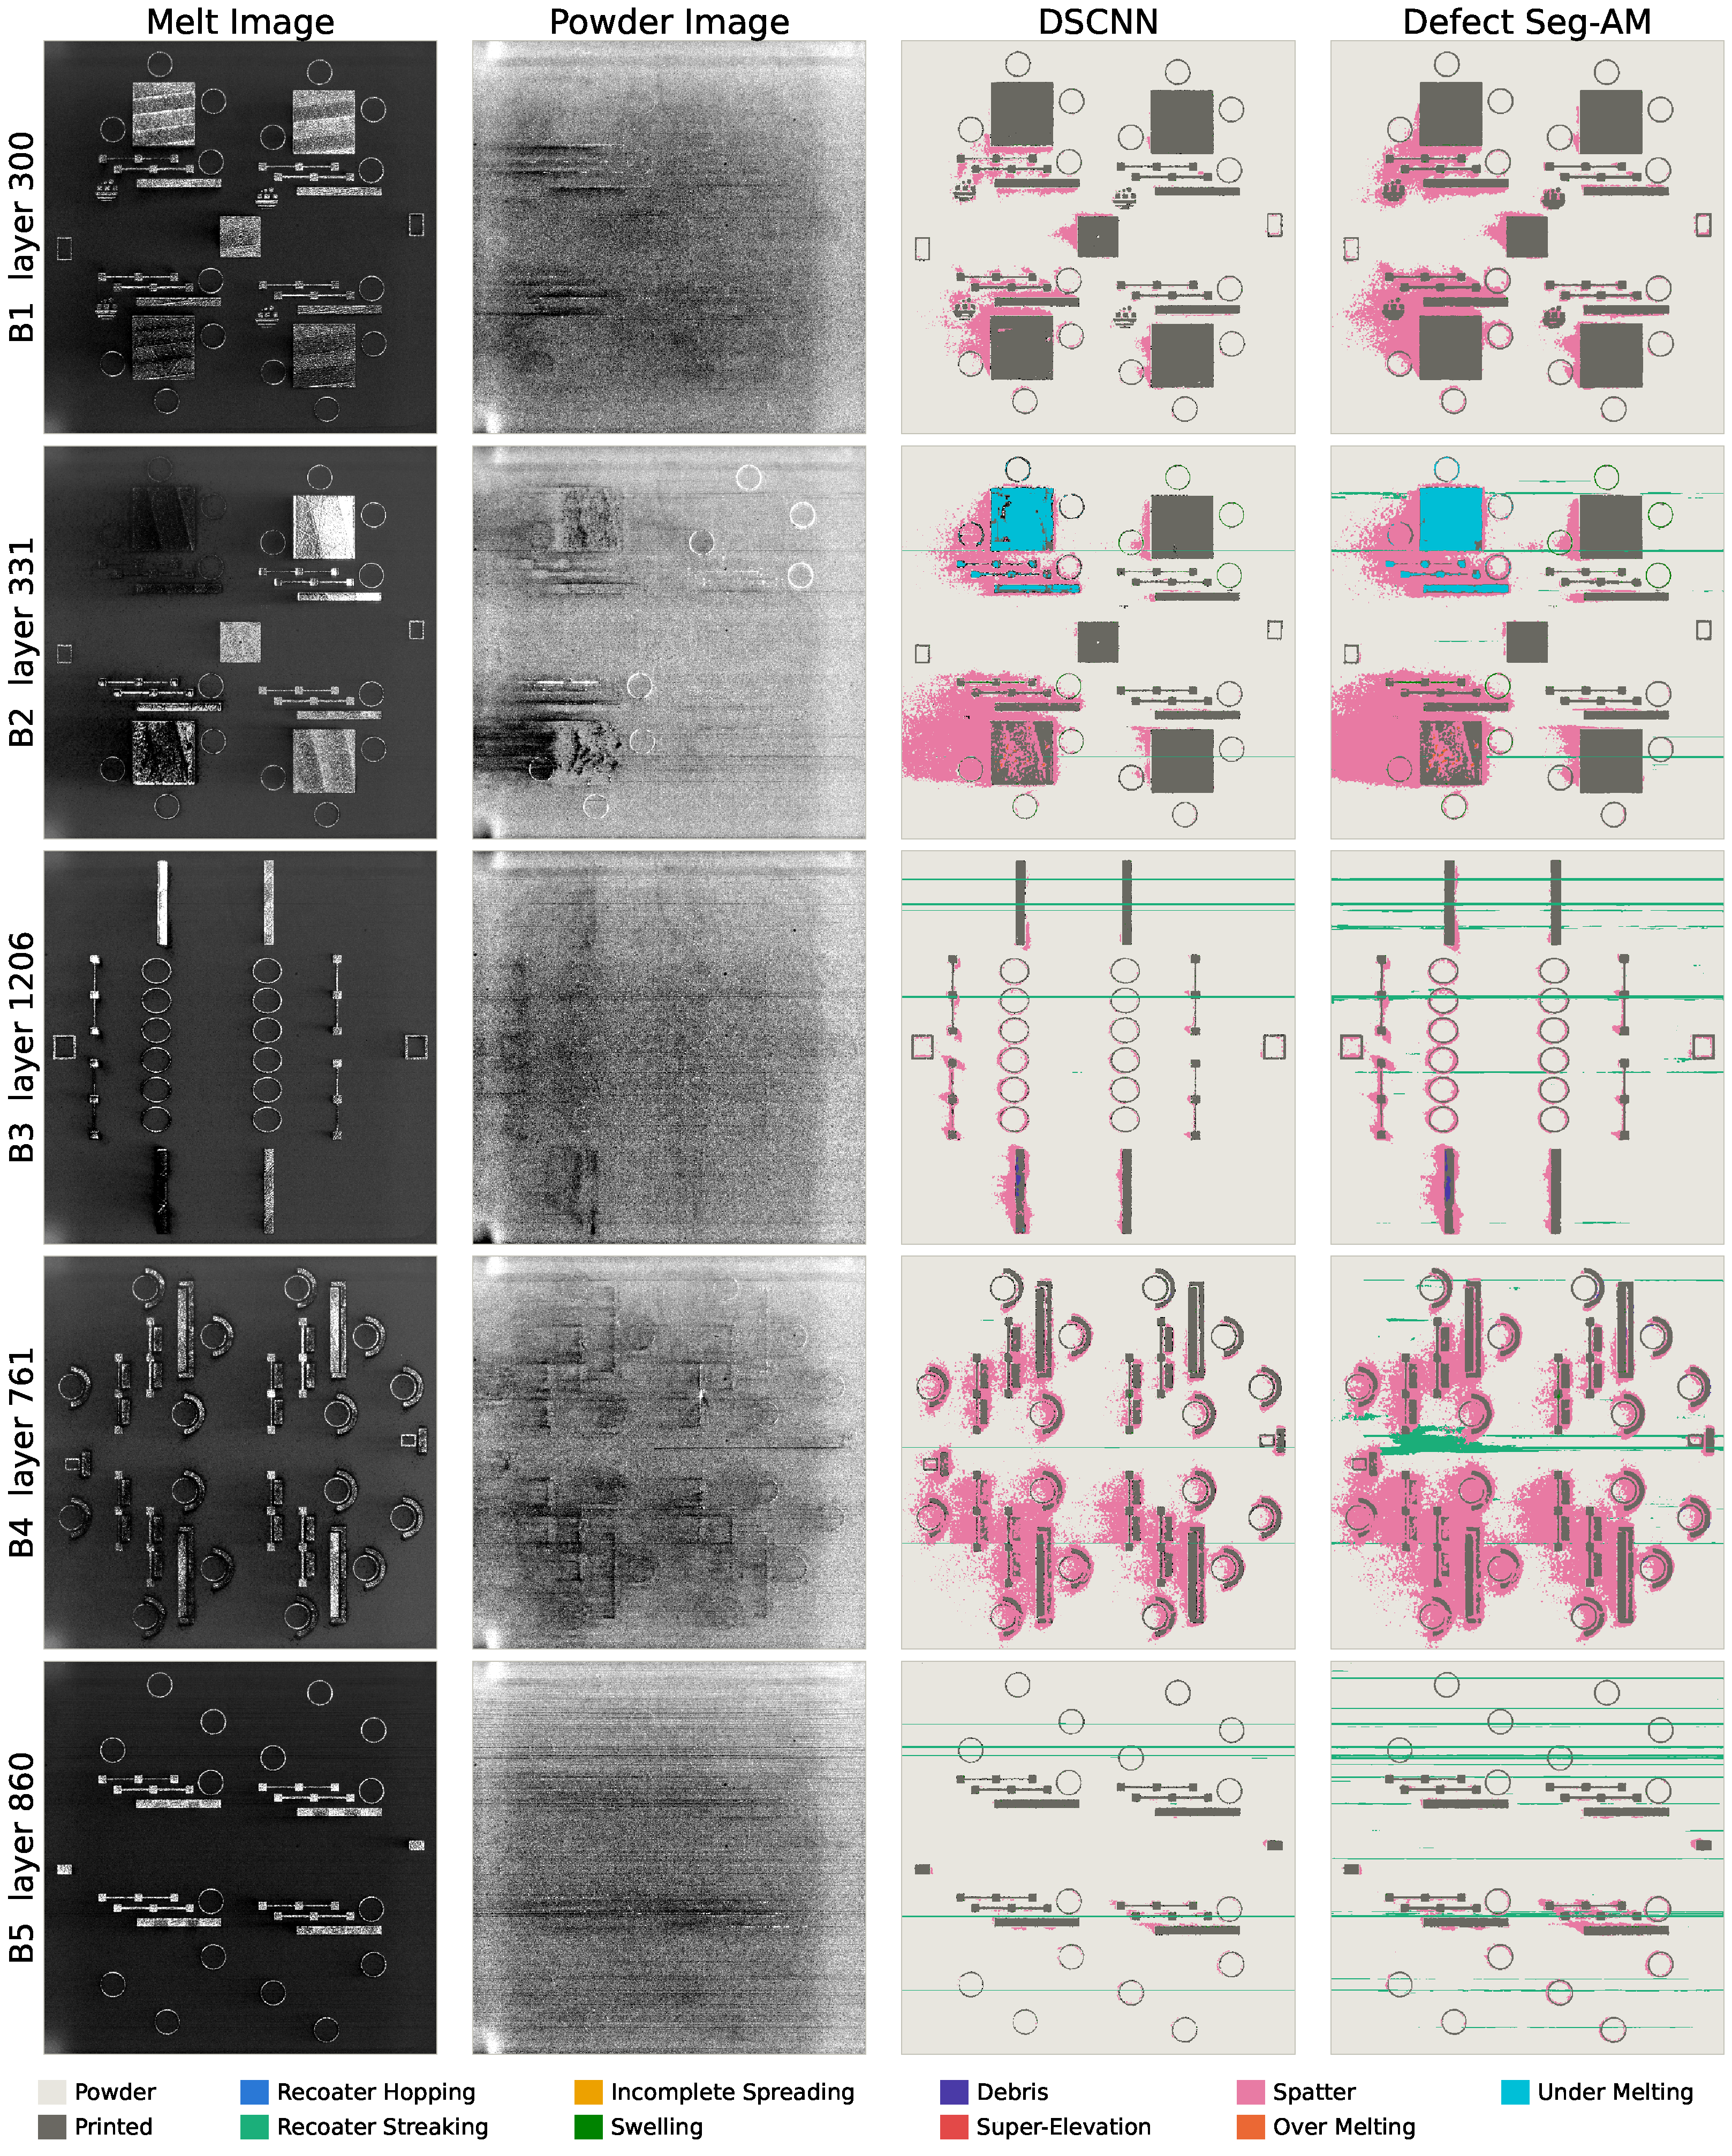
\includegraphics[width=\linewidth,height=0.80\textheight,keepaspectratio]{Figs/Image_Seg_Compare_DSCNN_vs_DefectSegAM.pdf}
\caption{다섯 개 ORNL 빌드 전체에서 샘플링한 대표 레이어에 대한 데이터셋
제공 production DSCNN 세그멘테이션(가운데)과 DefectSegAM(오른쪽)의 정성적
비교. 대응하는 원본 가시광 레이어 이미지를 왼쪽에 함께 나타냈다.
DefectSegAM 은 원본 이미지에서 관찰되는 것보다 다소 넓은 결함 영역을
예측하는 경미한 과탐지 경향을 보이지만, production DSCNN 이 부분적으로만
검출하거나 완전히 놓치는 Recoater Streaking 및 Spatter 영역을 일관되게
포착한다. 두 모델 모두 test-time augmentation 및 후처리 없이 나타냈다.}
\label{fig:qualitative-dscnn}
\end{figure}

% -------------------------------------------------------------------------
\subsection{다운스트림 인장 물성 사례 연구}
\label{sec:results-downstream}

ORNL 빌드에는 held-out 세그멘테이션 ground truth 가 없으므로, 해당
데이터셋에서는 DefectSegAM 과 production DSCNN 간의 직접적인 정확도 비교가
불가능하다. 따라서 본 연구에서는 두 세그멘테이션 소스를 그 출력의
다운스트림 유용성, 즉 그 외 조건이 동일한 인장 물성 예측 파이프라인에 각
소스가 물성 관련 정보를 얼마나 제공하는지를 기준으로 평가한다. 슈퍼복셀
집계, 소스별 채널 집합, 회귀 모델, 시편 단위 5-fold 교차검증 분할과 보고
방식은 모두 \ref{sec:setup-downstream}절의 프로토콜을 따른다.

표~\ref{tab:downstream}과 그림~\ref{fig:downstream}은 그 결과를 요약한다.
데이터셋 제공 DSCNN 맵을 사용하면 segmentation-only 예측기는 붕괴한다.
UTS RMSE $70.7 \pm 2.5$\,MPa 는 naive 전역 평균 예측기의 68.4\,MPa 보다
오히려 \emph{더 나쁘고}(3.4\,\% 악화), YS 역시 1.2\,\% 악화되며, UE 와 TE
는 각각 3.6\,\% 와 5.5\,\% 개선에 그친다. 이 붕괴의 원인은 맵 자체로
추적된다. 데이터셋 제공 세그멘테이션에서 유도한 슈퍼복셀 집계 결함 채널
피처의 평균은 약 0.001--0.008 에 불과하여 회귀기가 활용할 시편 간 분산이
사실상 남지 않으므로, 모델은 전역 평균을 출력하는 것 이상을 거의 할 수
없다. 동일한 DSCNN 채널에 대해 MLP 를 순환(recurrent) 인코더로 교체해도
같은 붕괴가 재현되며(UTS RMSE 64.8\,MPa), 이는 병목이 회귀 아키텍처가
아니라 세그멘테이션 소스임을 확인해 준다.

\begin{table}[t]
\centering
\caption{ORNL 데이터셋에서 \ref{sec:setup-downstream}절의 프로토콜(5-fold
시편 단위 교차검증, $N = 6{,}373$ 시편)로 평가한 segmentation-only VPPM
변형들의 시편 수준 RMSE. 항복강도(YS), 인장강도(UTS), 균일연신율(UE),
총연신율(TE)에 대해 보고한다. 학습되는 두 변형은 세그멘테이션 소스만
다르다. $\pm$ 는 다섯 개 fold 에 걸친 RMSE 의 표준편차를 나타내며,
naive(전역 평균) 예측기는 fold 가 없다.}
\label{tab:downstream}
\footnotesize
\begin{tabular}{lcccc}
\toprule
예측기 & YS (MPa) & UTS (MPa) & UE (\%) & TE (\%) \\
\midrule
Naive (전역 평균)              & 33.9 & 68.4 & 15.0 & 18.5 \\
DSCNN 기반 (데이터셋 제공)     & $34.3 \pm 1.4$ & $70.7 \pm 2.5$ & $14.5 \pm 0.2$ & $17.5 \pm 0.3$ \\
DefectSegAM 기반 (제안)        & $\mathbf{25.0 \pm 1.0}$ & $\mathbf{37.5 \pm 1.2}$ & $\mathbf{8.6 \pm 0.3}$ & $\mathbf{11.8 \pm 0.3}$ \\
\midrule
$\Delta$ vs.\ naive (DefectSegAM) & $-26.1\,\%$ & $-45.2\,\%$ & $-42.4\,\%$ & $-36.3\,\%$ \\
\bottomrule
\end{tabular}
\end{table}

\begin{figure}[t]
\centering
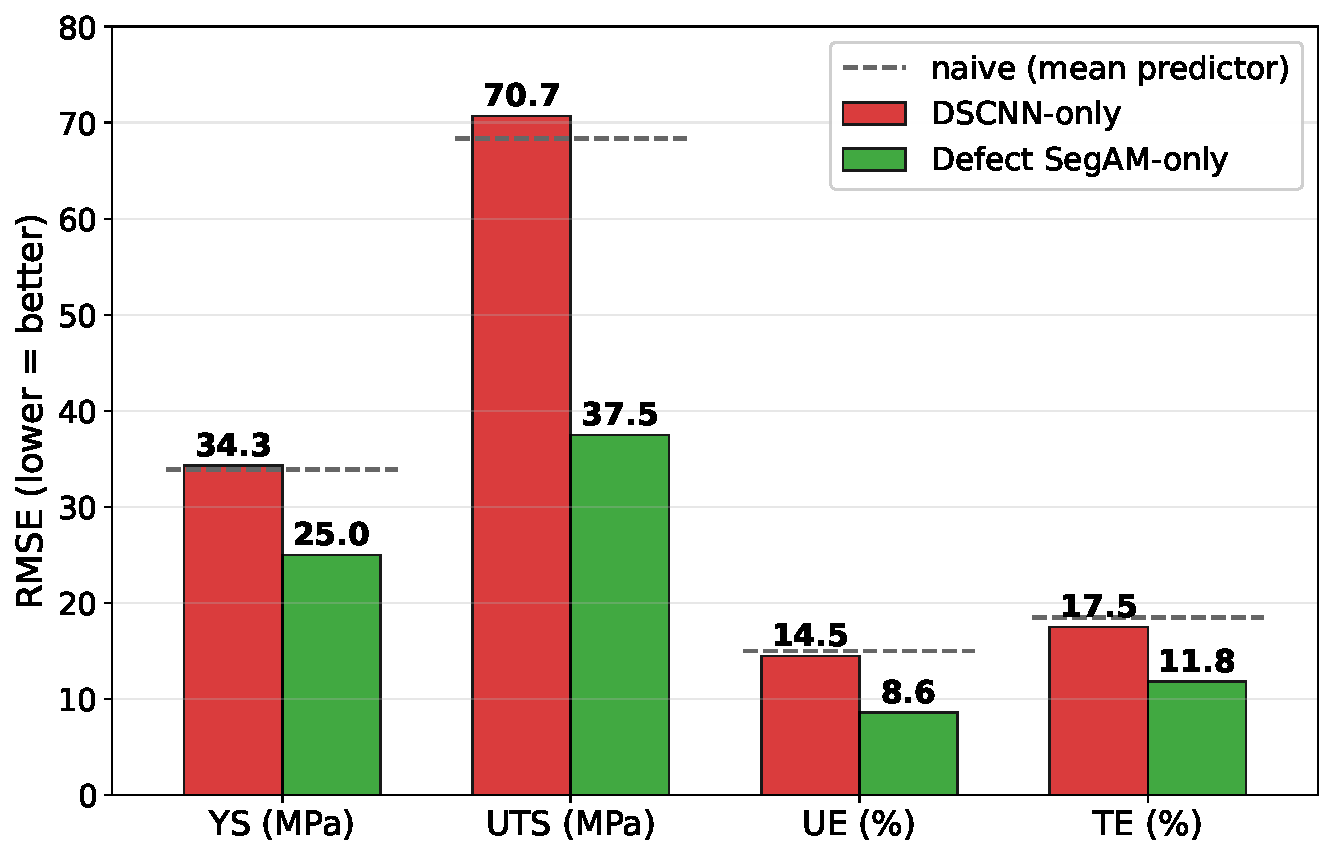
\includegraphics[width=\linewidth]{Figs/Graph_Seg_Compare_DSCNN_vs_DefectSegAM.pdf}
\caption{5-fold 시편 단위 교차검증에서 네 가지 인장 특성(YS, UTS, UE,
TE)에 대한 segmentation-only 물성 예측기의 시편 수준 RMSE. 막대는 DSCNN
기반 변형과 DefectSegAM 기반 변형을 비교하며, 점선은 naive 전역 평균
예측기를 표시한다. DSCNN 기반 변형은 naive 기준선을 개선하지 못하는
반면(YS 와 UTS 에서는 오히려 더 나쁨), DefectSegAM 기반 변형은 일관되게
그리고 큰 폭으로 기준선을 밑돈다. 수치 값은 표~\ref{tab:downstream}에
제시하였다.}
\label{fig:downstream}
\end{figure}

집계·모델·분할·정규화를 동일하게 유지한 채 세그멘테이션 소스만
DefectSegAM 으로 교체하면 결함 신호가 복원된다. DefectSegAM 기반 변형은
$25.0 \pm 1.0$\,MPa (YS), $37.5 \pm 1.2$\,MPa (UTS), $8.6 \pm 0.3$\,\%
(UE), $11.8 \pm 0.3$\,\% (TE) 의 RMSE 를 달성하며, 이는 naive 기준선 대비
각각 26.1\,\%, 45.2\,\%, 42.4\,\%, 36.3\,\% 의 감소이다. 다섯 개 UTS fold
의 RMSE 는 35.7--39.0\,MPa 의 좁은 범위에 분포한다. 참고로,
segmentation-only UTS 수치 37.5\,MPa 는 원 VPPM 논문에서 보고된 DSCNN 단독
결과(40.6\,MPa)~\cite{VPPM_Baseline}와 비견되며---실제로는 3.1\,MPa 더
낮고---센서·형상·스캔 경로 피처를 추가로 사용하는 본 연구의 21-피처
베이스라인 재현 결과(42.9\,MPa)보다도 낮다. 여기서 두 가지 결론이 따른다.
첫째, 이 데이터셋에서 segmentation-only VPPM 변형의 실패는 정적 8차원 집계
표현 자체의 본질적 한계가 아니라, 물성 관련 결함 정보를 너무 적게 담고
있는 세그멘테이션 소스의 결과이다. 둘째, 모든 변형이 동일한 시편 단위
교차검증 분할을 공유하므로, 이 대비는 세그멘테이션 품질에 대한 통제된,
teacher 독립적인 측정이 된다. 즉, DefectSegAM 은 데이터셋 제공 맵이
전달하지 못하는 물성 관련 결함 신호를 복원한다. 절대적인 RMSE 값은
leave-one-build-out 프로토콜에서는 달라질 수 있으나, 이
붕괴-복원(collapse-to-recovery) 대비는 다운스트림 물성 예측 파이프라인에서
DefectSegAM 을 세그멘테이션 소스로 채택하는 직접적인 실험적 근거가 된다.

% -------------------------------------------------------------------------
\subsection{계산 효율}
\label{sec:results-efficiency}

표~\ref{tab:efficiency}는 DefectSegAM 의 계산 비용을 프로파일링한 것으로,
배포 구성(ViT-B/14)과 이전 세대에서 사용한 ViT-S/14 변형의 frozen 및
학습 가능 파라미터 수를 보고한다(구성과 파라미터 분해는
\ref{sec:method-arch}절, 학습 하드웨어와 단계별 소요 시간은
\ref{sec:setup-impl}절). 학습은 GPU 당 배치 크기 4에서 GPU 당 약
20\,GB 의 메모리를 점유하는 것으로 측정되었다. 레이어당 추론
지연시간(latency)과 처리량(throughput)은 아직 벤치마크하지 않았다.
\TODO{DefectSegAM(8-way test-time augmentation 유무 각각)과 재구현 DSCNN
에 대해 동일한 하드웨어에서 단일 레이어 추론 지연시간과 초당 레이어
처리량을 측정하고, 표~\ref{tab:efficiency}의 해당 셀을 채울 것; 재구현
DSCNN 의 파라미터 수를 보고할 것.}

\begin{table}[t]
\centering
\caption{계산 비용 프로파일. 파라미터 수는 DefectSegAM 구성(frozen 인코더
/ 학습 가능 decoder 및 head)에 대해 정확한 값이며, 동일한 하드웨어에서의
추론 시간 측정은 미완료 상태이다. \TODO{지연시간·처리량 열을 기입할 것;
재구현 DSCNN 의 파라미터 수를 추가할 것.}}
\label{tab:efficiency}
\footnotesize
\begin{tabularx}{\textwidth}{@{}>{\raggedright\arraybackslash}Xcccc@{}}
\toprule
모델 & \makecell{Frozen\\파라미터} & \makecell{Trainable\\파라미터} & \makecell{입력 크기\\(px)} & \makecell{레이어당\\지연시간 (ms)} \\
\midrule
DefectSegAM (ViT-B/14, 배포 구성) & 86\,M & 14.6\,M & $1036 \times 1036$ & --- \\
DefectSegAM (ViT-S/14 변형)       & 22\,M & 13.4\,M & $1036 \times 1036$ & --- \\
DSCNN (재구현)~\cite{Scime2020DSCNN} & --- & --- & --- & --- \\
\bottomrule
\end{tabularx}
\end{table}

% -------------------------------------------------------------------------
\subsection{계획된 평가: held-out 사람 GT 비교, cross-machine 일반화,
ablation}
\label{sec:results-planned}

본 소절의 세 가지 평가---사람이 주석한 ground truth 상에서 재구현
DSCNN 과 비교하는 held-out 평가(\ref{sec:results-heldout}절),
cross-machine 일반화 연구(\ref{sec:results-crossmachine}절), 그리고 구성
요소 ablation(\ref{sec:results-ablation}절)---은 \ref{sec:setup}절에서
정의한 프로토콜을 따르지만 아직 수행되지 않았다. 이들에 대해서는 완전한
실험 스캐폴딩(scaffolding)을 제시하고 모든 정량 셀을 미기입(pending)
상태로 표시하며, 각 표는 결과가 확보되는 대로 채운다.

\subsubsection{사람 ground truth 상에서 재구현 DSCNN 과의 held-out 비교}
\label{sec:results-heldout}

본 연구의 핵심 정량적 주장은 DefectSegAM 의 학습 과정에서 어떠한 형태로도
사용된 적이 없는, 사람이 주석한 ground truth 상에서 확립할 예정이다. 평가
세트는 \ref{sec:setup-heldout-peregrine}절의 2025 Peregrine held-out
세트~\cite{Peregrine_v2025_TODO}이며, 베이스라인은
\ref{sec:setup-baselines}절의 재구현 DSCNN~\cite{Scime2020DSCNN}과 선택적
표준 베이스라인(U-Net, DeepLabV3+)의 설정을 따른다.
표~\ref{tab:heldout-main}은 결과 스캐폴드(scaffold)를 제시한다.
\TODO{held-out 평가를 수행할 것: (i) 2025 Peregrine 주석의 라벨 온톨로지가
12-class ORNL 공간과 호환되는지 검증하고 매핑을 문서화할 것; (ii) 원 논문에서
DSCNN 하이퍼파라미터를 옮겨 적어 동일한 코퍼스로 재구현 모델을 학습할 것;
(iii) 표~\ref{tab:heldout-main}의 모든 셀을 공정 기술별 mIoU 와 픽셀
정확도로 채울 것.}

\begin{table}[t]
\centering
\caption{본 연구의 어떤 학습에도 쓰이지 않은 2025 Peregrine held-out
세트(\ref{sec:setup-heldout-peregrine}절)에서의 세그멘테이션 성능. 모든
모델은 \ref{sec:setup-corpora}절의 동일한 코퍼스로 학습한다. mIoU 는
support 가 0이 아닌 클래스들에 대한 mean intersection-over-union 이며,
L-PBF 와 BJ 는 각각 Concept Laser M2 부분집합과 ExOne Innovent 부분집합을
나타낸다. 모든 항목은
미기입(pending) 상태이다. \TODO{held-out 평가 수행 후 기입할 것; 2025 주석의
12-class 공간으로의 라벨 온톨로지 매핑을 확인할 것.}}
\label{tab:heldout-main}
\footnotesize
\begin{tabular}{lcccc}
\toprule
모델 & \makecell{mIoU\\(L-PBF)} & \makecell{mIoU\\(BJ)} & \makecell{mIoU\\(all)} & \makecell{Pixel acc.\\(all)} \\
\midrule
DSCNN (재구현)~\cite{Scime2020DSCNN} & --- & --- & --- & --- \\
U-Net~\cite{Ronneberger2015UNet}            & --- & --- & --- & --- \\
DeepLabV3+~\cite{Chen2018DeepLabV3Plus}     & --- & --- & --- & --- \\
DefectSegAM (제안 모델)                     & --- & --- & --- & --- \\
\bottomrule
\end{tabular}
\end{table}

\subsubsection{Cross-machine 일반화}
\label{sec:results-crossmachine}

동결(frozen)된 파운데이션 모델 피처 위에 DefectSegAM 을 구축한 핵심 동기는
장비·소재·카메라 구성을 가로지르는 전이(transfer)이다. 이 주장을 ORNL
생태계 밖에서 검증하기 위해, 어떠한 장비별 재학습도 없이 모든 학습 소스에
부재한 장비들의 분말 도포(recoating) 이미지에 대해 모델을 평가한다. 평가
세트는 \ref{sec:setup-heldout-crossmachine}절의 저자 수집 cross-machine
세트(Veltz M160/M280 및 EOS 장비)의 정의를 따르며, 2025 Peregrine 세트는
같은 절에서 밝힌 이유로 포함하지 않는다.
표~\ref{tab:crossmachine}은 스캐폴드를 제시하며, 모든 셀에서 재구현
DSCNN 이 비교 모델로 사용된다. \TODO{Veltz M160/M280 및 EOS 이미지를
수집하고 픽셀 라벨링할 것(레이어 수, 소재, 카메라 사양, 라벨링 프로토콜
문서화 예정); 세 개 장비 부분집합 모두에서 두 모델을 실행하고
표~\ref{tab:crossmachine}을 채울 것.}

\begin{table}[t]
\centering
\caption{학습 중 보지 못한 장비에 대한 cross-machine 일반화. 각 행은
held-out 사람 주석 recoating 이미지의 한 장비 부분집합이며, 두 모델 모두
장비별 재학습을 받지 않는다. $\Delta$mIoU 는 DefectSegAM 에서 DSCNN 을 뺀
값이다. 모든 항목은 미기입(pending) 상태이다. \TODO{cross-machine 데이터
수집 및 평가 후 기입할 것; 부분집합별 레이어 수, 소재, 카메라 사양을
문서화할 것.}}
\label{tab:crossmachine}
\footnotesize
\begin{tabularx}{\textwidth}{@{}>{\raggedright\arraybackslash}Xlccc@{}}
\toprule
장비 & 공정 & \makecell{DSCNN\\mIoU} & \makecell{DefectSegAM\\mIoU} & $\Delta$mIoU \\
\midrule
Veltz M160                        & PBF        & --- & --- & --- \\
Veltz M280                        & PBF        & --- & --- & --- \\
EOS 장비 \TODO{모델명}            & PBF        & --- & --- & --- \\
\bottomrule
\end{tabularx}
\end{table}

\subsubsection{Ablation 연구}
\label{sec:results-ablation}

DefectSegAM 의 아키텍처와 학습 레시피에는 여섯 가지 설계 결정이 포함되어
있으며, 각각의 개별 기여는 \ref{sec:results-heldout}절과 동일한 held-out
사람 ground truth 상에서 분리하여 확인할 예정이다:
(i)~이중 이미지 입력 --- 용융 직후(melt) 이미지 $I_0$ 만 또는 분말
도포(powder) 이미지 $I_1$ 만 입력하여 ablation; (ii)~명시적 변화
단서(change cue) --- 식~\eqref{eq:forward}의 융합에서
$\mathbf{F}^{(1)}_s-\mathbf{F}^{(0)}_s$ 차분 항을 제거하여 두 피처 맵의
concatenation 만 남김; (iii)~Stage-1 의사 라벨(pseudo-label) 사전학습 ---
무작위 초기화된 decoder 를 전문가 주석에 직접 미세조정하여 ablation;
(iv)~class-aware 레이어 샘플링 --- 균일 샘플링으로 대체;
(v)~Copy-Paste 증강~\cite{Ghiasi2021CopyPaste} --- 증강 체인에서 제거;
그리고 (vi)~백본 용량 --- ViT-B/14 인코더를 이전 모델 세대에서 사용한
ViT-S/14 인코더로 교체. 여기에 더해 학습
없이 추론 시에만 적용되는 두 가지 옵션, 즉 (vii)~8-way test-time
augmentation 과 (viii)~\ref{sec:method-inference}절의 두 가지 휴리스틱
후처리 규칙의 효과를 같은 held-out 세트에서 정량화한다.
표~\ref{tab:ablation}은 스캐폴드를 제시한다. \TODO{ablation 대상 구성
요소를 제외하고는 동일한 2-stage 레시피로 일곱 가지 구성을 학습하고,
전체 모델에 TTA 와 후처리를 각각 추가한 두 가지 추론 시 옵션과 함께
held-out 사람 GT mIoU 로 표~\ref{tab:ablation}을 채울 것.}

\begin{table}[t]
\centering
\caption{표~\ref{tab:heldout-main}의 held-out 사람 주석 테스트 세트에서
평가한 DefectSegAM 의 구성 요소 ablation. 각 학습 변형은 전체 모델 대비
정확히 하나의 구성 요소만 변경하며, 추론 시 옵션 행은 전체 모델의 학습된
가중치를 그대로 두고 test-time augmentation(TTA) 또는 후처리 규칙만
추가한 것이다. $\Delta$mIoU 는 첫 번째 행 대비 변화량이다. 모든 항목은
미기입(pending) 상태이다. \TODO{ablation 실행 후 기입할 것.}}
\label{tab:ablation}
\footnotesize
\begin{tabular}{lcc}
\toprule
구성 & mIoU & $\Delta$mIoU \\
\midrule
DefectSegAM (전체 모델, 단일 forward)        & --- & ---  \\
\midrule
\multicolumn{3}{@{}l}{\emph{학습 변형}}\\
단일 이미지: 용융 직후 $I_0$ 만              & --- & --- \\
단일 이미지: 도포 직후 $I_1$ 만              & --- & --- \\
차분 항 $\mathbf{F}^{(1)}_s-\mathbf{F}^{(0)}_s$ 제거 & --- & --- \\
Stage-1 pseudo-label 사전학습 제거           & --- & --- \\
Class-aware 샘플링 제거                      & --- & --- \\
Copy-Paste 증강 제거                         & --- & --- \\
ViT-S/14 백본 (22\,M frozen)                 & --- & --- \\
\midrule
\multicolumn{3}{@{}l}{\emph{추론 시 옵션 (전체 모델)}}\\
$+$ 8-way TTA                                & --- & --- \\
$+$ 8-way TTA $+$ 후처리 규칙 1--2           & --- & --- \\
\bottomrule
\end{tabular}
\end{table}

% =========================================================================
% Section 6 — Discussion
% Fragment for \input from main.tex (no preamble).
% =========================================================================
\section{고찰}
\label{sec:discussion}

% -------------------------------------------------------------------------
\subsection{라벨 희소성 하에서 frozen 파운데이션 피처가 유효한 이유}
\label{sec:discussion-frozen}

Powder bed fusion 의 픽셀 단위 결함 세그멘테이션을 규정하는 제약은 모델
용량이 아니라 주석 공급이다. 본 연구가 사용할 수 있는 전체 전문가
ground-truth 코퍼스는 여덟 개 장비/소재
소스~\cite{Peregrine_v2021_03,Peregrine_v2022_10}에 걸친 125개 주석
레이어로 구성되며, 이 중 98개는 L-PBF, 27개는 binder jet 이다. 수천만 개
파라미터를 갖는 현대적 세그멘테이션 네트워크를 이러한 코퍼스로
처음부터(from scratch) 학습하면, 코퍼스에 나타난 소수의 빌드·카메라·조명
조건에 대한 심각한 과적합을 초래하게 된다. DefectSegAM 은 이 제약을
정칙화(regularization)만으로가 아니라 구조적으로 해결한다. register
토큰~\cite{Darcet2024Registers}으로 안정화된 86\,M 파라미터 DINOv2
인코더~\cite{Oquab2024DINOv2}는 전체가 동결(frozen)된 채 유지되므로,
전문가 주석은 융합 projection, decoder, head 의 14.6\,M 학습 가능
파라미터만 형성하면 된다. 인코더의 표현은 자연 이미지에 대한 대규모
자기지도학습(self-supervision)으로 학습된 것이어서 특정 powder-bed
카메라에 독립적이며, 학습 문제는 이러한 범용 피처에서 결함 온톨로지로의
매핑을 학습하는 것으로 환원된다. 이는 소규모 라벨 세트에 잘 부합하는 전이
학습~\cite{Pan2010TransferLearning}의 한 형태이다. 2-stage 레시피는 이
효과를 배가한다. 12{,}607개의 의사 라벨(pseudo-label) ORNL 레이어에 대한
Stage-1 사전학습은 decoder 에 전체 결함 온톨로지에 대한 조밀하고 저렴한
지도 신호를 제공하므로, 125개의 전문가 주석 레이어는 decoder 를 초기화하는
데가 아니라 교정하는 데 사용된다. 표본 수 대 파라미터 수의 관점에서
보면, Stage-1 은 12{,}607개 레이어 $\times$ $1036 \times 1036$ 픽셀, 즉
약 $1.4 \times 10^{10}$개의 의사 라벨 픽셀을, Stage-2 는 125개 레이어의
최대 약 $1.3 \times 10^{8}$개의 주석 픽셀(ignore 픽셀 제외 전)을
14.6\,M 개의 학습 파라미터에 대응시킨다. 다만 인접 픽셀 간의 강한 공간
상관 때문에 유효 표본 수는 이 픽셀 수보다 훨씬 작으며, 이 점이 인코더를
동결하고 학습 대상을 decoder 로 한정하는 설계를 뒷받침한다. 태스크별 라벨 없이 promptable 파운데이션
모델을 AM 결함 세그멘테이션에 활용한 연구~\cite{Era2025SAM}도 같은 방향을
가리킨다. 본 설계는 학습된 decoder 를 통해 파운데이션 피처를 고정된
11-class 온톨로지에 특화시킨다는 점에서 다르며, 이로써 다운스트림 정량
파이프라인으로의 직접 통합이 가능해진다. frozen 피처 논증의 결정적 시험은
\ref{sec:results-crossmachine}절의 cross-machine 평가이다. 가설이 옳다면,
모든 학습 소스에 부재한 Veltz 및 EOS 이미징 조건에 직면했을 때
DefectSegAM 은 전체를 학습한 합성곱 베이스라인보다 더 완만하게 성능이
저하되어야 한다.
\TODO{표~\ref{tab:heldout-main}--\ref{tab:ablation}이 채워지면 이 논증을
정량적으로 재검토할 것.}

% -------------------------------------------------------------------------
\subsection{의사 라벨 teacher 편향}
\label{sec:discussion-teacher}

Stage-1 코퍼스는 Peregrine 플랫폼에 배포된 production
DSCNN~\cite{Scime2020DSCNN}이 라벨링한 것이며,
\ref{sec:results-agreement}절에서 강조하였듯이 두 단계 모두에서 모델 선택
역시 검증 빌드의 DSCNN 유래 라벨을 기준으로 점수화된다. 이는 체계적인
위험을 초래한다. teacher 가 일관되게 저지르는 오류는 ORNL 빌드에서 계산할
수 있는 모든 일치도(agreement) 지표에 보이지 않으며, 선택 기준이 teacher
를 교정하는 체크포인트보다 teacher 를 모방하는 체크포인트를 선호할 수
있다. 세 가지 관찰이 이 위험의 범위를 한정한다. 첫째, Stage-2 미세조정은
teacher 의 지도 신호를 여덟 개 소스의 사람 주석으로 대체하며, 그중 일곱
개는 의사 라벨이 생성된 Concept Laser M2/SS~316L 구성이 아닌 다른 장비
또는 소재에서 온 것이다. 따라서 전문가 라벨이 teacher 와 불일치하는 모든
곳에서 student 는 teacher 로부터 명시적으로 멀어지도록 이끌린다. 둘째,
그림~\ref{fig:qualitative-dscnn}의 정성적 비교는 DefectSegAM 이 teacher
로 수렴하는 것이 아니라, production 모델이 놓치는 Recoater Streaking 및
Spatter 영역을 포착하는 등 일관된 방향으로 teacher 로부터 벗어남을
보여준다. 셋째, 그리고 가장 중요하게,
\ref{sec:results-downstream}절의 다운스트림 사례 연구는 teacher 와
독립적이다. 6{,}373개 시편의 인장 물성은 어느 세그멘테이션 모델과도
무관하며, 이 외부 기준에서 student 의 맵은 teacher 의 맵보다 실질적으로 더
많은 물성 관련 정보를 담고 있다(동일한 파이프라인에서 UTS RMSE 37.5 대
70.7\,MPa). 따라서 teacher 로부터의 이탈은 적어도 총량 수준에서는 노이즈가
아니라 개선이다. 그럼에도 일치도 통계는 픽셀 수준 정확도를 결코 보증할 수
없으며, 이것이 재구현되어 동일하게 학습된 DSCNN 을 상대로 한
\ref{sec:results-heldout}절의 held-out 사람 GT 평가가 본 논문의
세그멘테이션 주장에 대한 결정적 실험으로 남는 이유이다.

% -------------------------------------------------------------------------
\subsection{Ground truth 희소성과 클래스 불균형}
\label{sec:discussion-imbalance}

\ref{sec:setup}절의 클래스 통계는 학습과 평가 양쪽에 엄격한 한계를
부과한다. 극단적인 경우 Recoater Hopping 은 다섯 개 ORNL 빌드 전체에 걸쳐
25개의 참조 픽셀만을 제공하며, 여러 클래스가 거의 전적으로 단일 빌드에
집중되어 있다(B1.2 에 Over Melting 의 99.8\,\% 와 Under Melting 의
99.9\,\%; B1.5 에 Super-Elevation 의 98\,\%; B1.3 에 Debris 의 90\,\%).
학습 측 완화책---역빈도 class-aware 샘플링, 희소 클래스 성분의 Copy-Paste
증강~\cite{Ghiasi2021CopyPaste}, 그리고 제곱근 역빈도 클래스 가중치를
적용한 focal loss~\cite{Lin2017FocalLoss}---은 최적화 과정에서의 노출
문제를 다루지만, 어떠한 샘플링 기법도 존재하지 않는 평가 support 를
만들어낼 수는 없다. 고정 검증 빌드 B1.1 은 11개 클래스 중 4개에 대해 참조
픽셀이 사실상 전무하므로, 해당 빌드의 모든 내부 지표는 이들 클래스에 대해
아무것도 말해 주지 못한다. 이것이
표~\ref{tab:results-agreement-perclass}의 다중 빌드 분석이 용융 에너지
클래스에 유의미한 support 를 갖는 유일한 빌드인 B1.2 에 의존하는 이유이며,
정상 조건 빌드에서의 단일 숫자 mIoU 값이 모델이 학습한 바를 체계적으로
과소평가하는 이유이다.

구속 조건이 최적화가 아니라 전문가 라벨 희소성이라는 증거는 본 모델의 이전
세대에서 나온다. 여덟 개 전문가 주석 소스에 대한 v2 세대 모델(ViT-S/14
백본, 8-class head---본 논문에서 제안하는 모델이 아님)의
leave-one-source-out 교차검증은 fold 평균 mIoU 0.253(평균 픽셀 정확도
0.894)을 산출하였으며, fold 별 mIoU 는 0.139 에서 0.346 에 걸쳐 있었고
가장 희소한 클래스들의 fold 평균 IoU 는 0 에 가까웠다(Over Melting
$\approx 0$, Debris $\approx 0.003$, Spatter 0.056). 이 수치들은 본 연구가
공략하도록 설계된 도메인 갭과 라벨 희소성을 보여주는 동기 부여 증거로서만
인용한다---이 결과들은 ViT-B 백본, 11-class 온톨로지, class-aware 샘플러,
Copy-Paste 증강 이전의 것이다---그리고 fold 별 mIoU 평균이 해당 fold 의
검증 소스에 부재한 클래스를 제외하므로 fold 간 분모가 달라 절대 수준을
과잉 해석해서는 안 된다는 방법론적 유의점을 함께 밝혀 둔다.
\ref{sec:results-ablation}절의 ablation 은 DefectSegAM 설계가 이 결손을
얼마나 회복하는지 정량화할 예정이다.
\TODO{표~\ref{tab:ablation}이 채워지면 이 동기 부여 베이스라인과
명시적으로 비교할 것.}

% -------------------------------------------------------------------------
\subsection{Binder-jet/L-PBF 도메인 갭}
\label{sec:discussion-domaingap}

같은 v2 세대 교차검증은 도메인 갭의 위치를 특정한다. 여섯 개 L-PBF fold
의 평균 mIoU 는 0.288(픽셀 정확도 0.904)이었던 반면, 두 개 binder-jet
fold 의 평균은 0.145(픽셀 정확도 0.867)였으며, binder-jet 소스의 Printed
클래스 IoU 는 0.02--0.07 로 붕괴하였다. binder-jet 소스는 비전 모델에
중요한 거의 모든 측면에서 L-PBF 소스와 다르다---센서(20\,MP 가시광 카메라,
그중 하나는 적색 조명, 대 1--5\,MP 가시광 시스템), 표면 외관(바인더로
응고된 분말 대 용융된 금속), 결함 물리(roller streaking, short feed,
cornrows 대 용융 기인 이상)---따라서 이 붕괴는 dataset
shift~\cite{Quinonero2009DatasetShift,Torralba2011DatasetBias}의 교과서적
사례이다. 미세조정에 사용할 수 있는 전문가 주석 binder-jet 레이어가
27개뿐이므로 두 공정 기술 간의 동등한 성능을 기대하지는 않는다.
표~\ref{tab:heldout-main}의 공정 기술별 열은 이 갭을 평균 내어 감추는 대신
정직하게 보고하도록 설계되어 있다. L-PBF 내부에서는, 계획된 Veltz
M160/M280 및 EOS 평가가 같은 질문의 더 완화되었지만 실용적으로 핵심적인
버전---하나의 공정 계열 내에서 장비와 카메라를 가로지르는 전이---을
검증하며, frozen 백본 설계는 바로 이를 견뎌 내도록 특별히 의도된 것이다.

% -------------------------------------------------------------------------
\subsection{결함 분류 체계의 함의}
\label{sec:discussion-taxonomy}

\ref{sec:method-taxonomy}절의 외형 기준 체계는 본 논문의 실험에 쓰이지
않았지만, 11-class 온톨로지로 얻은 결과 중 일부는 그 설계와 모순되지
않는다. 첫째, 표~\ref{tab:results-agreement-perclass}에서 B1.2 의
Super-Elevation 일치도 IoU 는 0.0043 에 그친다. 같은 150개 레이어의
confusion matrix 를 보면 참조 Super-Elevation 픽셀 1{,}396개 중
86.7\,\%(1{,}210개)가 Swelling 으로 예측되었다. 반대로 참조 Swelling 픽셀
852{,}040개 중 Super-Elevation 으로 예측된 것은 34개로 사실상 없다. 두
클래스의 ORNL 정의는 각각 변형된 프린팅 재료와 프린팅 영역 위의 분말 피복
부족이지만, 저자들의 관찰로는 Powder 이미지에서 모두 파트가 분말 위로
드러난 유사한 형상으로 나타나 구별하기 어렵다. 이 혼동 관찰은 support 가
극히 작은 B1.2 에서의 것이고 teacher 자신의 일관성에 대해서는 말해 주지
않지만, 두 클래스를 통합 클래스 Super Elevation 으로 합치는 제안과
부합한다. 다만 이 혼동은 클래스 불균형만으로도 설명된다. 같은 150개
레이어에서 모델이 Super-Elevation 으로 예측한 픽셀은 총 707개로, student
가 이 클래스를 거의 출력하지 않는 희소 클래스 붕괴에 해당하므로, 이 혼동
관찰은 두 클래스의 외형이 유사하다는 근거가 아니라 통합 제안과 양립한다는
정도로만 해석해야 한다. 두 클래스를 합친 일치도 IoU 는 0.6043
으로 Swelling 단독(0.6038)과 거의 같으므로, 통합의 효과는 일치도 수치가
아니라 참조 라벨의 일관성과 희소 클래스 하나의 제거에 있다. 또한
Super-Elevation 픽셀의 98\,\% 가 집중된 B1.5 는 샘플링된 150개 레이어에서
support 가 0 이므로, 이 클래스가 실제로 발생하는 빌드에서의 분리 가능
여부는 이 분석으로 알 수 없다. 통합이 실제로 라벨 노이즈를 줄이는지는
재주석 후 주석자 간 일치도로 확인해야 한다.
둘째, \ref{sec:method-inference}절의 후처리 규칙 2(Printed 마스크 위의
Spatter 를 Over Melting 으로 재라벨링)는 제안 체계보다 먼저 도입된
휴리스틱이지만 제안 체계의 영역 기준 판별과 같은 취지이며, 학습 라벨이 그
기준으로 주석된다면 같은 구분을 모델이 직접 학습하게 된다. 셋째, 본 논문의
핵심 결과 중 하나인 B1.2 의 Under Melting 일치도(IoU 0.8643)는 저에너지
밀도라는 공정 파라미터로 정의된 클래스에 대한 것이어서, 외형 기준 원칙
아래에서는 이 클래스의 처리가 아직 확정되지 않았다. 이 일치도는 teacher 와
student 가 같은 패턴을 표시함을 뜻할 뿐이고 해당 픽셀의 99.9\,\% 가 B1.2
한 빌드에 집중되어 있으므로, 주석자가 적용할 수 있는 외형 판정 기준의
존재를 보증하지 않는다. 제안 체계로 전환하면 이 결과는 재정의된 클래스에
대해 다시 평가되거나, 제외될 경우 더 이상 보고되지
않는다(\ref{sec:results}절에서 비교한 이전 세대 모델 v3 의 10-class 공간은
Under Melting 을 뺀 것으로, 제안 체계의 10개 클래스와는 무관하다). Over
Melting 에도 같은 주의가 필요하다. 제안 체계의 Over Melting 은 파트 영역
위의 거뭇한 영역이라는 외형으로 재정의되므로,
\ref{sec:results-agreement}절에서 keyhole 전조로 해석한 11-class Over
Melting(B1.2 일치도 IoU 0.4715)과 같은 대상이 아니다. 따라서 DefectSegAM
기반 다운스트림 변형(\ref{sec:setup-downstream}절)이 사용하는 Over
Melting 과 Under Melting 채널도 클래스 재정의와 재학습 뒤에 다시 평가해야
한다. 넷째, 제안 체계는 데이터 가용성의 제약을 그대로 물려받는다.
Powder Collapse 에는 어떤 코퍼스에도 라벨이 없고, Recoater Hopping 은 ORNL
코퍼스에 25픽셀뿐이며, Spatter 와 Over Melting 의 사람 주석을 늘릴 수 있는
native ``Soot'' 의 분할은 파트 마스크가 비어 있지 않은 소수 레이어(maraging
steel 9개 레이어, 전체 Soot 주석의 약 9\,\%)에만 적용 가능하고 마스크 경계
오차를 감수해야 한다. 따라서 제안 체계의 검증은 재주석과 재학습을
전제로 한다.
\TODO{제안 체계로 재주석한 뒤 재학습하고
표~\ref{tab:results-agreement-perclass}를 재산출할 것.}

% -------------------------------------------------------------------------
\subsection{타당성에 대한 위협}
\label{sec:discussion-validity}

본 결과를 제한하는 한계들을 요약한다. (i)~현재 ORNL 빌드에서 가용한 모든
정량적 세그멘테이션 수치는 production DSCNN 과의 일치도(agreement)
통계이지 정확도가 아니다. 이 통계는 teacher 와 student 가 공유하는 오류를
탐지할 수 없으며, 본 논문의 정확도 주장은 \ref{sec:results-heldout}절과
\ref{sec:results-crossmachine}절의 미수행 held-out 평가에 달려 있다.
(ii)~다운스트림 사례 연구는 시편 단위 교차검증을 사용하므로 모든 fold 가
모든 빌드의 시편을 포함한다. 더 엄격한 leave-one-build-out 프로토콜에서는
절대 RMSE 값이 달라질 수 있으나, 모든 변형이 동일한 분할을 공유하므로
세그멘테이션 소스 간 붕괴-복원 대비는 분할 설계의 영향을 받지 않는다.
(iii)~다운스트림 증거는 단일 소재와 장비(Concept Laser M2 의
SS~316L~\cite{ORNL_CoRegistered_Dataset}) 및 하나의 물성군만을 다루며, 그
일반화는 검증되지 않았다. (iv)~통합 온톨로지는 각 소스의 native 클래스를
11-class 공간으로 매핑하며, 대응 클래스가 없는 클래스는 ignore 픽셀로서
loss 에서 제외된다(native Misprint 포함). 따라서 소스 간의 체계적인 라벨링
관례 차이는 명시적으로 모델링하지 않는 라벨 노이즈로 남는다. 이 노이즈의
일부는 온톨로지 자체가 원인 기준과 외형 기준을 섞어 쓰는 데서 비롯하며,
\ref{sec:method-taxonomy}절의 외형 기준 체계는 이를 줄이도록 설계되었으나 본
논문의 어떤 결과에도 아직 적용되지 않았다(\ref{sec:discussion-taxonomy}절).
(v)~DSCNN
재구현의 충실성은 원 논문~\cite{Scime2020DSCNN}에서 옮겨 적은
하이퍼파라미터에 의존한다. 문서화가 불충분한 세부 사항은 베이스라인 비교의
교란 요인이 되며, 이는 재구현의 구성을 전부 보고함으로써 완화할 예정이다.
(vi)~보고된 모든 일치도 수치와 그림은 단일 forward pass 를 사용한
것이다. test-time augmentation(TTA)과 두 가지 추론 시 후처리 규칙은 본
논문의 어떤 결과에도 적용되지 않았으므로 그 정량적 효과는 아직 측정되지
않았다. (vii)~Stage-1 학습은
random seed 를 고정하지 않으므로 전체 파이프라인의 실행 간(run-to-run)
분산은 정량화되지 않았다. Stage-2 는 고정 seed 를 사용한다. \TODO{held-out
평가와 함께 seed 민감도 및 TTA·후처리의 정량적 효과를 정량화할 것.}

% =========================================================================
% Section 7 — Conclusion
% Fragment for \input from main.tex (no preamble).
% =========================================================================
\section{결론}
\label{sec:conclusion}

본 논문은 register 를 갖춘 frozen DINOv2 ViT-B/14 인코더(86\,M 파라미터)를
14.6\,M 학습 가능 파라미터의 DPT 스타일 다중 스케일 decoder 와 결합한,
powder bed fusion 적층제조를 위한 레이어 단위 결함 세그멘테이션 모델
DefectSegAM 을 제시하였다. 모델은 레이어당 두 카메라 뷰---용융
직후(post-melting) 이미지와 도포 직후(post-spreading) 이미지---를 모두
입력받아, 두 피처 맵과 그 차분을 채널 방향으로 연결(concatenation)하는
명시적 변화 단서(change cue)를 통해 네 개의 transformer 깊이에서 융합한
뒤, $1036 \times 1036$ 해상도의 11-class 픽셀 단위 결함 맵을 디코딩한다.
라벨 효율적인 2-stage 레시피는 먼저 production DSCNN 이 의사 라벨링한
12{,}607개 ORNL 빌드 레이어로 decoder 를 사전학습한 뒤, laser powder bed
fusion 과 binder jetting 에 걸친 여덟 개 장비/소재 소스에서 추출한 단
125개의 전문가 주석 레이어로 미세조정하며, 역빈도 class-aware 샘플링,
희소 결함 클래스의 Copy-Paste 증강, 그리고 focal loss 를 통해 15.33
billion 개의 powder 픽셀에서 가장 희소한 결함 클래스의 25 픽셀까지 이르는
극단적인 클래스 불균형에 대응한다. 아울러 실험과는 별도로, 데이터셋 어휘에
혼재된 원인 기준과 외형 기준을 분리하여 레이어 이미지에 나타난 특징을 판정
기준으로 정의한 결함 8종(Under Melting 처리 확정 전 기준)과 배경 2종의
분류 체계를 향후 주석을 위해 제안하고 기존 라벨 공간 및 ASTM E3353-22
표준 용어와의 대응을 명시하였다.

ORNL Co-Registered 빌드에서 DefectSegAM 은 production 모델이 신뢰할 만한
곳에서는 이를 가깝게 따르면서도, 일관되고 결함에 민감한 방향으로
이탈한다. 결함 다수(defect-rich) 빌드 B1.2 에서 이전 내부 세대의
0.4291--0.4455 대비 0.5047 의 일치도(agreement) mIoU 를 달성하며, 이는
lack-of-fusion 및 keyhole 기공의 전조인 용융 에너지 클래스 Under
Melting(0.8643)과 Over Melting(0.4715)이 주도한 결과이다. 이 맵들의
가치는 세그멘테이션과 전혀 별개인 외부 태스크에서 입증되었다. 6{,}373개
시편에 대한 그 외 조건이 동일한 segmentation-only 인장 물성 파이프라인에서
데이터셋 제공 DSCNN 맵을 DefectSegAM 으로 교체하자, 인장강도(UTS) RMSE 가
naive 전역 평균 기준선 68.4\,MPa 보다도 나쁜 70.7\,MPa 에서 37.5\,MPa 로
감소하였으며, 항복강도(YS), 인장강도(UTS), 균일연신율(UE),
총연신율(TE) 전반에 걸쳐 해당 기준선 대비 26--45\,\% 의 일관된 감소를
보였다. 이 붕괴-복원(collapse-to-recovery) 대비는 다운스트림 물성 예측을
지배하는 것이 집계 표현의 단순성이 아니라 세그멘테이션 소스의 정보량임을
보여준다. 결정적인 세그멘테이션 수준 비교---2025 Peregrine 릴리스의
held-out 사람 ground truth 와 수집이 진행 중인 저자 라벨링 Veltz
M160/M280 및 EOS 이미지에서 충실히 재구현된 DSCNN 을 상대로 하는
비교---는 본 논문에서 완전하게 명세되었으며 그 수행은 향후 과제로 남아
있다. \TODO{\ref{sec:results}절에 스캐폴딩된 held-out, cross-machine,
ablation 평가를 완료할 것.}

여러 방향이 자연스럽게 이어진다. 첫째, 실시간 배포이다. frozen 인코더
설계는 체크포인트당 14.6\,M 학습 가능 파라미터만 저장하지만, 세그멘테이션이
생산 장비의 도포(recoating) 간격 내에 완료되도록 레이어당 추론 지연시간을
벤치마크하고 필요하다면 단축해야 한다. 둘째, 폐루프(closed-loop) 제어이다.
빌드 도중 가용한 결함 맵은 재도포(re-coating)나 파라미터 조정과 같은 교정
조치를 촉발하여 모니터를 액추에이터로 전환할 수 있다. 11개 클래스 중 어느
것이 이러한 개입을 게이트할 만큼 신뢰할 수 있는지를 정량화하는 것은
held-out 평가가 답하기 시작할 열린 질문이다. 셋째, 범위의 확장이다. 전문가
주석 코퍼스를 현재의 125개 레이어 너머로---특히 도메인 갭이 가장 큰
binder jetting 과 추가적인 합금·장비에 대해---확장하고, DefectSegAM 을
SS~316L 이외 소재의 물성 예측 파이프라인에 결합하는 것은 본 연구에서
입증된 라벨 효율성이 계속 증가하는 powder bed fusion 시스템의 보급 기반
전반에 걸쳐 누적적으로 작동하는지를 시험하게 될 것이다. 넷째, 분류 체계의
확정이다. \ref{sec:method-taxonomy}절의 외형 기준 체계로 재주석하고
재학습하면 Swelling 과 Super-Elevation 처럼 외형이 유사하여 구별하기 어려운
클래스 쌍은 하나로 합쳐지지만, 신설되는 Powder Collapse 와 ORNL 코퍼스에
25픽셀뿐인 Recoater Hopping 은 여전히 신규·희소 주석에 의존한다. 또한
기존 Over Melting 라벨은 새 정의를 만족하는지 레이어별로 재검토한 뒤
재매핑해야 하고, Under Melting 의 처리도 확정되어야 한다. 체계의 효과는
주석자 간 일치도와 재산출된 per-class 일치도로 검증해야 하며, 이는 향후
과제로 남는다.


% ---- Elsevier-required end matter ---------------------------------------
% Order follows Elsevier publishing practice: CRediT -> competing interest ->
% data availability -> acknowledgements -> funding -> generative-AI
% declaration (immediately before the references, per the June 2026 policy).
% Headings are the journal's fixed English titles; prose stays Korean.

\section*{CRediT authorship contribution statement}
\textbf{Taehoon Lee}: Conceptualization, Methodology, Software,
Investigation, Data curation, Writing -- original draft, Writing -- review
\& editing. \TODO{저자 명단이 확정된 후 CRediT 명세를 완성할 것.}

\section*{Declaration of competing interest}
저자들은 본 논문에 보고된 연구에 영향을 미친 것으로 보일 수 있는
경쟁적 금전적 이해관계나 개인적 관계가 없음을 선언한다.

\section*{Data availability}
본 연구에서 분석한 데이터는 공개 저장소에서 이용 가능하다. ORNL
Co-Registered In-Situ and Ex-Situ 데이터셋(Peregrine
v2023-11)~\cite{ORNL_CoRegistered_Dataset}과 Peregrine 기계학습 릴리스
v2021-03~\cite{Peregrine_v2021_03}, v2022-10~\cite{Peregrine_v2022_10},
2025~\cite{Peregrine_v2025_TODO}는 참고문헌에 명시된 DOI를 통해 Oak Ridge
Leadership Computing Facility 데이터 저장소에서 공개적으로 이용 가능하다.
저자가 수집 중인 Veltz M160/M280 및 EOS 교차 장비 이미지는 현재 수집이
진행 중이며, 수집과 라벨링이 완료되는 시점에 그 가용성을 명시할
예정이다. \TODO{코드 및 학습된 체크포인트의 공개 여부(저장소 URL 또는
DOI)를 명시할 것; 저자 수집 교차 장비 세트의 최종 가용성을 명시할 것.}

\section*{Acknowledgements}
\TODO{감사의 글(해당 시)을 추가할 것.}

\section*{Funding}
\TODO{연구비 출처를 다음 두 형식 중 하나로 명시할 것: (i) ``This work
was supported by [기관명] [과제번호].''와 함께 후원자의 연구 설계, 자료
수집·분석·해석, 집필, 투고 결정 관여 여부를 한 문장으로; 또는 (ii)
``This research did not receive any specific grant from funding agencies in
the public, commercial, or not-for-profit sectors.''}

\section*{Declaration of generative AI and AI-assisted technologies in the
manuscript preparation process}
본 원고를 준비하는 과정에서 저자들은 \TODO{도구/서비스 이름과 버전, 사용
목적(예: 한국어 초고의 문장 교정과 구조 정리, 영문 번역, LaTeX 정리)을
확정할 것}을 사용하였다. 이 도구를 사용한 후 저자들은 필요한 내용을
검토하고 수정하였으며, 출판되는 논문의 내용에 대한 전적인 책임을 진다.

\bibliographystyle{elsarticle-num}
\bibliography{refs}

\end{document}
